\documentclass[11pt,a4paper]{book}
\usepackage[utf8]{inputenc}
\usepackage[french]{babel}
\usepackage[left=2cm,right=2cm,top=2cm,bottom=2cm]{geometry}
\usepackage{fancyhdr}
\usepackage{appendix}
\usepackage{amsmath}
\usepackage{amsfonts}
\usepackage{amssymb}
\usepackage{stmaryrd}
\usepackage{mathrsfs}
\usepackage{graphicx}
\usepackage[ruled,vlined, french, algochapter]{algorithm2e}
\usepackage{ntheorem}
\usepackage[table,dvipsnames,svgnames]{xcolor}
\usepackage[framemethod=tikz]{mdframed}
\usetikzlibrary{shadows,shadings}
\usepackage{sectsty}
\usepackage{multicol}
\usepackage{hyperref}
\usepackage{listings}
\usepackage{float}
\usepackage[explicit]{titlesec}
\usepackage{colortbl}
\usepackage{enumitem}
\usepackage{tikz} %Tikz !
\usepackage{multirow}
\usepackage{ulem}
\usepackage{hhline}
\usetikzlibrary{automata, positioning, arrows}
\usetikzlibrary{shapes,shapes.geometric}
\usepackage{cancel}

\usepackage{xcolor}
\definecolor{mGreen}{rgb}{0,0.6,0}
\definecolor{mGray}{rgb}{0.5,0.5,0.5}
\definecolor{mPurple}{rgb}{0.58,0,0.82}
\definecolor{backgroundColour}{rgb}{0.95,0.95,0.92}

\tikzset{elliptic state/.style={draw,ellipse}}

% En-tête et pied de page
\newcommand{\mask}[1]{}

\pagestyle{fancy}
\renewcommand\headrulewidth{1pt}
\fancyhead[L]{Leçons d'Informatique}
\fancyhead[R]{Préparation à l'Agrégation d'Informatique 2022}
\fancyfoot[R]{\tiny $\copyright$ 2024 Martinez 2022 M. Marin}

\setcounter{tocdepth}{1} 



%Design des théorèmes
\usepackage{framed}


\newmdtheoremenv[
outerlinewidth=1pt,
innerlinewidth=0pt,
roundcorner=2pt,
linecolor=black,
shadow=true,
tikzsetting={shading=axis,top color=gray!10},
innertopmargin=1\baselineskip,
skipabove={\dimexpr0.5\baselineskip+\topskip\relax},
needspace=3\baselineskip ,
frametitlefont={\sffamily\bfseries},
]{theorem}%
{\color{BrickRed}Théorème}[chapter]

\newmdtheoremenv[
outerlinewidth=1pt,
innerlinewidth=0pt,
roundcorner=2pt,
linecolor=black,
shadow=true,
tikzsetting={shading=axis,top color=gray!10},
innertopmargin=1\baselineskip,
skipabove={\dimexpr0.5\baselineskip+\topskip\relax},
needspace=3\baselineskip ,
frametitlefont={\sffamily\bfseries},
]{proposition}%
{\color{IndianRed}Proposition}[chapter]

\newmdtheoremenv[
outerlinewidth=1pt,
innerlinewidth=0pt,
roundcorner=2pt,
linecolor=black,
shadow=true,
tikzsetting={shading=axis,top color=gray!10},
innertopmargin=1\baselineskip,
skipabove={\dimexpr0.5\baselineskip+\topskip\relax},
needspace=3\baselineskip ,
frametitlefont={\sffamily\bfseries},
]{lemma}%
{\color{IndianRed}Lemme}[chapter]

\newmdtheoremenv[
outerlinewidth=1pt,
innerlinewidth=0pt,
roundcorner=2pt,
linecolor=black,
shadow=true,
tikzsetting={shading=axis,top color=gray!10},
innertopmargin=1\baselineskip,
skipabove={\dimexpr0.5\baselineskip+\topskip\relax},
needspace=3\baselineskip ,
frametitlefont={\sffamily\bfseries},
]{corollary}%
{\color{IndianRed}Corollaire}[chapter]


\newmdtheoremenv[
outerlinewidth=1pt,
innerlinewidth=0pt,
roundcorner=2pt,
linecolor=black,
shadow=true,
tikzsetting={shading=axis,top color=gray!10},
innertopmargin=1\baselineskip,
skipabove={\dimexpr0.5\baselineskip+\topskip\relax},
needspace=3\baselineskip ,
frametitlefont={\sffamily\bfseries},
]{definition}%
{\color{ProcessBlue}Définition}[chapter]


\newmdtheoremenv[
outerlinewidth=1pt,
innerlinewidth=0pt,
roundcorner=2pt,
linecolor=black,
shadow=true,
tikzsetting={shading=axis,top color=gray!10},
innertopmargin=1\baselineskip,
skipabove={\dimexpr0.5\baselineskip+\topskip\relax},
needspace=3\baselineskip ,
frametitlefont={\sffamily\bfseries},
]{principe}%
{\color{DarkGreen}Principe}[chapter]


\makeatletter
\def\newframedGtheorem#1{%
\theoremprework{
\renewcommand*\FrameCommand{%
  {\color{DimGrey}\vrule width 3pt \hspace{2.5pt}}}
  \framed}%
\theorempostwork{\endframed}%
\newtheorem@i{#1}%
}
\makeatother
%%%


%Définition des différents environnements
\newframedGtheorem{rem}{\color{DimGrey}Remarque}[chapter]
\newframedGtheorem{com}{\color{Blue}Commentaire}[chapter]
\newtheorem{example}{\textbf Exemple}[chapter]
\newtheorem{exercise}{\color{orange}\textbf Exercice}[chapter]
\newtheorem{idee}{\textbf Idée}[chapter]
\newtheorem{temps}{\color{gray} Temps}[chapter]


\newtheorem{notion}{\textbf Notion}[chapter]
\newtheorem{algo}{\textbf Algorithme}[chapter]


\newtheorem{impl}{\textbf Implémentation}[chapter]
\newtheorem{syntaxe}{\textbf Syntaxe}[chapter]
\newtheorem{appl}{\textbf Application}[chapter]
\newtheorem{idea}{\textbf Idée}[chapter]

\newenvironment{proof}[1][\unskip]{\noindent \textit{Démonstration #1. }}{\hfill $\square$ \\}


%Gestion de la hierarchie
\setcounter{secnumdepth}{3}

\renewcommand{\familydefault}{\sfdefault}
\renewcommand{\thesection}{\arabic{section}}
\renewcommand{\thesubsection}{\Roman{subsection}}
\renewcommand{\thesubsubsection}{\Alph{subsubsection}}


\makeatletter
\renewcommand{\@chapapp}{Leçon}
\makeatother


%En-tête des leçons 
% utilisation : \debut{Auteurs}{niveau}{pré-requis}{références}
\newcommand\debut[4]{
\noindent \textbf{Auteur\textperiodcentered e\textperiodcentered s:} #1  \\
\noindent\textbf{Niveau :} #2 \\
\noindent\textbf{Pré-requis :} #3 \\
\noindent\textbf{Références :} #4 \\
}

%En-tête des développements 
% utilisation : \debut{Auteurs}{références}
\newcommand\dev[2]{
\noindent \textbf{Auteur\textperiodcentered e\textperiodcentered s:} #1  \\
\noindent\textbf{Références :} #2 \\
}

%Commande personnalisées
\newcommand{\N}{\ensuremath{\mathbb{N}}}
\newcommand{\overarrow}[1]{\smash{\overset{#1}{\longrightarrow}}}
\newcommand*\circled[1]{\tikz[baseline=(char.base)]{
		\node[shape=circle,draw,inner sep=2pt] (char) {#1};}}

%Pour le listing de code
\lstset{
frame = single, 
framexleftmargin=1pt,
literate=
{à}{{\`a}}1
{é}{{\'e}}1
{è}{{\`e}}1
{ô}{{\^o}}1}

\lstset{escapeinside={<@}{@>}}

\definecolor{lightpink}{HTML}{f7d1d5}
%Éviter le saut de page après un chapitre
\renewcommand{\cleardoublepage}{\newpage}
\newcommand\countme{\refstepcounter{\thechapter}\thechapter}

\lstdefinestyle{CStyle}{
	backgroundcolor=\color{backgroundColour},   
	commentstyle=\color{mGreen},
	keywordstyle=\color{magenta},
	numberstyle=\tiny\color{mGray},
	stringstyle=\color{mPurple},
	basicstyle=\footnotesize,
	breakatwhitespace=false,         
	breaklines=true,                 
	captionpos=b,                    
	keepspaces=true,                 
	numbers=left,                    
	numbersep=5pt,                  
	showspaces=false,                
	showstringspaces=false,
	showtabs=false,                  
	tabsize=2,
	language=C
}
%Copyright




\begin{document}

%\begin{titlepage}
    \newgeometry{left=5cm,right=1cm,bottom=1cm}
    \noindent
\begin{flushright}
\vspace*{-3cm}

\includegraphics[scale=0.5]{Headers/logo-ens.png}
 
 \vspace{2cm}
\end{flushright}
    {\LARGE \textsf{École Normale Supérieure de Lyon} }
    \par
    \noindent
    \makebox[0pt][l]{\rule{1.3\textwidth}{1pt}}
    \par\medskip
    {\noindent \huge\textbf{\textsf{Leçons d'Informatique}}}
    \par\medskip
    {\noindent\huge\textbf{\textsf{Agrégation 2022} }}


    \par\vspace*{1cm}
    {\noindent\huge\textsf{Marin Malory, Sorci Émile, Rousseau Guillaume, Bertrand Jules} }
    

\vfill%

\end{titlepage}

\restoregeometry
\nopagecolor

\tableofcontents

%\chapter*{Préface}
%\input{Préface/préface.tex}

\part{Leçons}

\chapter{Exemples de méthodes et outils pour la correction des programmes.} \label{L1}
\dev{Emile Martinez}{}{}{}

La conjecture de Syracuse est un problème ouvert de Mathématiques : \\
La suite $u$ définie par : $\left\{ \begin{array}{l}
	u_0 = a \in \N^*\\
	u_{n+1} = \left\{\begin{array}{ll}
		\dfrac{u_n}{2} & \text{si } u_n \text{ est pair}\\
		3u_n+1 & \text{sinon}
	\end{array}\right.
\end{array}\right.$ finie-t-elle toujours par le cycle $1,2,4$ ? (toujours = pour tout $a\in \N^*$)\\

Cela revient à savoir si l'algorithme \\
\begin{algorithm}[H]
	\caption{Syracuse(a)}
	$u \gets a$\\
	\Tq{$u$ est une nouvelle valeur}{
		\eSi{$u$ est pair}
		{
			$u\gets \dfrac{u}{2}$
		}{
			$u \gets 3u+1$
		}
	}
	\Retour{$u$}
\end{algorithm}
renvoie toujours 1, 2 ou 4.

\subsection{Terminaison}
Une première question est de savoir si \texttt{Syracuse} finit (ne boucle pas à l'infini) sur toute entrée.

\begin{definition}
	Prouver la terminaison d'un algorithme revient à prouver que sur toute entrée il termine
\end{definition}

\begin{rem}
	On se limite parfois aux entrées valides (pour Syracuse, $a \in \N^*$ par exemple)
\end{rem}

\begin{example}
	\enspace \\ \\
	\begin{minipage}{0.4\linewidth}
		\begin{lstlisting}
Tant que a > 0:
    a = a - 1
		\end{lstlisting}
	\end{minipage} \quad \begin{minipage}{0.5\linewidth}
		Termine sur tout entrée si on n'autorise pas $a$ à valoir $+\infty$, sinon ne termine pas sur toute entreé.
	\end{minipage}
\end{example}

\begin{definition}
	Un \textbf{variant} est une fonction des variables, à valeurs dans $\N$ qui décroit strcitement :
	\begin{itemize}
		\item à chaque passage dans la boucles pour les algorithmes itératifs
		\item à chaque appel récursif pour les algorithmes récursifs.
	\end{itemize}
\end{definition}

\begin{example} \enspace \\ \\ \label{1-2}
	\begin{minipage}{0.5 \linewidth}
		\begin{algorithm}[H]
			\caption{pgcd($a$,$b$)}
			\Tq{$\min(a,b) > 0$}{
				\eSi{$a<b$}
				{
					$b\gets b-a$
				}
				{
					$a\gets a - b$
				}
			}
			\Retour{$\max(a,b)$}
		\end{algorithm}
	\end{minipage} \quad \begin{minipage}{0.4 \linewidth}
		La fonction \texttt{pgcd(a,b)} qui calcule le pgcd de $a$ et $b$ pour $a, b \in \N$ admet comme variant $a+b$ (qui est en effet toujours positif, et décroit à chaque fois)
	\end{minipage}
\end{example}

\begin{proposition}
	\label{1-1}
	Si une boucle a un variant de voucle, alors elle s'éxecute un nombre fini de fois. De même pour un algorithme récursif.
\end{proposition}

\begin{example}
	pgcd($a$,$b$) termine pout tout $(a,b)\in \left(\N^*\right)^2$
\end{example}

\begin{rem}
	Si un algorithme termine sur toute entrée, il existe toujours un variant, mais il peut être difficile à trouver (ou à prouver)
\end{rem}

\begin{com}
	Il suffit de prendre comme variant le nombre d'étapes de calcul restantes en focntion de l'état de la mémoire
\end{com}

\begin{example} \enspace \\
	\begin{minipage}{0.4\linewidth}
		On définit $ack(n,m)$ pour $n,m\in \N$ par \\ $\left\{\begin{array}{l}
			ack(0,m) = m+1\\
			ack(n, 0) = ack(n-1, 1)\\
			ack(n,m) = ack(n-1, ack(n, m-1))
		\end{array}\right.$
	\end{minipage}\quad
	\begin{minipage}{0.55\linewidth}
		\begin{algorithm}[H]
			\caption{ack($n$,$m$)}
			\eSi{$n=0$}{
				\Retour{$m+1$}
			}{
				\eSi{$m = 0$}
				{
					\Retour{ack($n-1$, $m$)}
				}
				{
					\Retour{ack($n-1$, ack($n$, $m-1$))}
				}}
		\end{algorithm}
	\end{minipage} \\Il n'est pas immédiat que $ack$ termine.
\end{example}

\begin{definition}
	On dit qu'un ordre est un \textbf{ordre bien fondé} si toute suite décroissante est stationnaire
\end{definition}

\begin{example}
	$\N$ avec l'ordre naturel est bien fondé 
\end{example}

\begin{proposition}
	Les ordres produit et lexicographiques d'ordre bien fondés sont bien fondés
\end{proposition}

\begin{example}
	Un ordre total sur un ensemble fini est bien fondé, donc l'ordre alphabétique est bien fondé (c'est un ordre lexicographique)
\end{example}

\begin{definition}
	On étend alors la définition du variant aux fonctions à valeurs dans un bon ordre.
\end{definition}

\begin{proposition}
	La propriété \ref{1-1} reste valide avec notre définition étendue du variant
\end{proposition}

\begin{example}
	Pour ack, $(n,m)$ est un variant dans $\N^2$ avec l'ordre lexicographique, donc ack termine
\end{example}

\subsection{Correction partielle}

Une autre question pour \texttt{Syracuse} est de savoir si on peut tomber sur un autre cycle que 1,2,4 et donc renvoyer autre chose que 1,2 ou 4.

\begin{definition}
	On appelle \textbf{spécification} d'un algorithme deux propriétés $P_1$ sur les entrées (pré-condition) et $P_2$ sur les sorties (post-condition)
\end{definition}

\begin{example}
	Pour Syracuse, $P_1 : «a\in \N»$ et $P_2 : «\text{Syracuse}(a) \in \{1,2,4\}»$
\end{example}

\begin{definition}
	On dit qu'un algorithme est \textbf{partiellement correct} si pour toute entrée vérifiant la pré-condition, si l'algorithme termine, la sortie vérifie la post-condition.
\end{definition}

\begin{example}
	L'algorithme de l'exemple \ref{1-2} est partiellement correct si la pré-condition est «$a\in \N, b \in \N$» et la post-condition «\texttt{pgcd(a,b)} renvoie le PGCD de a et de b» \label{1-3}
\end{example}

\subsubsection{Correction partielle des algorithmes impératifs}

Pour prouver la correction partielle des langages impératifs, on utilise un invariant de boucle.

\begin{definition}
	Un invariant de boucle est une propriété qui est vrai avant la boucle, et si elle est vraie quand on commence un tour de boucle, alors elle l'est quand on le finit.
\end{definition}

\begin{proposition}
	Si un invariant de boucle est valide, alors il est vrai après la boucle, et la condition d'arrêt de la boucle est fausse.
\end{proposition}

\begin{example}
	Pour pgcd, «$PGCD(a,b) = PGCD(a_0, b_0)$» où $a_0$ et $b_0$ sont les valeurs initiales de \texttt{a} et \texttt{b}, est un invariant valide.
	
	A la fin de l'exécution, on a donc $\min(a,b) = 0$ et $PGCD(a,b) = PGCD(a_0, b_0) = PGCD(\min(a,b), \max(a,b)) = PGCD(0, \max(a,b)) = \max(a,b)$. D'où l'assertion de l'exemple \ref{1-3}
\end{example}

\subsubsection{Correction partielle des algorithmes récursifs}


\begin{principe}
	Pour prouver la correction partielle d'un algorithme récursif, on vérifie que si \begin{itemize}[label=$\bullet$]
		\item la pré-condition est vérifiée
	\end{itemize}, alors
	\begin{itemize}[label=$\bullet$] 
		\item on ne fait que des appels récursifs où les arguments vérifient la pré-condition
		\item Si la post-condition des appels récursifs est vérifiée, alors celle de notre appel est vérifiée
	\end{itemize}
	\label{1-5}
\end{principe}

\begin{theorem}
	Si le principe \ref{1-5} est respecté, alors l'algorithme est partiellement correct.
\end{theorem}

\begin{example}
	\label{1-7}
	exp($a$,$n$) pour $a,n\in \N$ renvoie $a^n$.\\\\
	\begin{minipage}{0.5\linewidth}
		\begin{algorithm}[H]
			\caption{exp($a$, $n$)}
			\eSi{$n=0$}{
				\Retour{$1$}
			}{
				$x =$exp($a$, $n$)\\
				\eSi{$n$ est pair}
				{
					\Retour{$x*x$}
				}
				{
					\Retour{$x*x*a$}
				}
			}
			\end{algorithm}
	\end{minipage} \quad \begin{minipage}{0.4\linewidth}
		Précondition : «\texttt a est un flottant et \texttt n un entier».\\
		Postcondition : $\texttt{exp(a,n)} = a^n$.\\
		Alors, la pré-condition est valide à chaque appel, et comme $a^n = a^{\lceil n \rceil} * a^{\lfloor n \rfloor}$, le principe \ref{1-5} est respecté dans tous les cas donc l'algorithme est partiellement correct.
	\end{minipage}
\end{example}

\subsection{Correction}

La conjecture de Syracuse dit donc que notre fonction Syracuse termine, et quand elle termine est correcte (i.e. partiellement correcte).

\subsubsection{Cas général}

\begin{definition}
	Quand un programme termine sur toute entrée valide et est partiellement correct, on dit qu'il est correct, ou encore totalement correct.
\end{definition}

\begin{example}\enspace\\
	\begin{algorithm}[H]
		\caption{fusion($L_1$, $L_2$)}
		$res \gets []$\\
		$i,j \gets 0$\\
		\Tq{
			$i < |L_1|$	et $j < |L_2|$
		}{
			\eSi{$L_1[i] < L_2[j]$}{
				$res$.ajouter($L_1[i]$) \\
				$i \gets i + 1$
			}{
				$res$.ajouter($L_2[j]$) \\
				$j \gets j + 1$
			}
		}
		Ajouter le reste de $L_1$ et de $L_2$ à $res$\\
		\Retour{$res$}
	\end{algorithm}

	\begin{algorithm}[H]
		\caption{tri\_fusion($L$)}
		$n \gets |L|$\\
		\Si{$n\leq 1$}{
			\Retour{$L$}
		}
		$L_1, L_2 \gets$ partionner($L$)\\
		\Retour{fusion( tri\_fusion($L_1$), tri\_fusion($L_2$) )}
	\end{algorithm}
\end{example}

\textbf{Developpement \ref{D?}} Correction totale de tri\_fusion.\\

Néanmoins, ce n'est pas toujours facile. La conjecture de Syracuse est toujours un problème ouvert. Et c'est parfois même pire.

\begin{theorem}
	La correction partielle et la terminaison sont indécidables. \label{1-6}
\end{theorem}

\textbf{Developpement \ref{D?}} Preuve du théorème \ref{1-6}

\subsubsection{Cas des algorithmes récursifs}

Dans le cas des algorithmes récurifs, on fait régulièrement la correction totale directement.

\begin{proposition}
	SI $(E, \preceq)$ est un ordre bien fondé, alors toutes parties non vides à un élément minimal (plus grand que personne)
\end{proposition}

\begin{theorem}
	\label{1-4}
	Soit $(A, \preceq)$ un ensemble muni d'un ordre bien fondé et $\mathcal P$ une propriété sur $A$, alors $\forall x \in A, \, (\forall y \in A, \, y \preceq A \enspace \Rightarrow \enspace \mathcal P(y) \Rightarrow \mathcal P(x)) \enspace \Rightarrow \enspace \forall x ,\, \mathcal P(x)$
\end{theorem}

\begin{rem}
	Cela étend le principe de réccurence forte sur $\N$
\end{rem}

L'ordre bien fondé nous donne alors le variant et la propriété l'invariant. On montre alors la terminsaison et la correction partielle en même temps.

\begin{example}
	Dans l'exemple \ref{1-6}, la propriété $\mathcal P(n)$ : «exp($a$,$n$)$ = a^n$» vérifie les bypothèses du théorème \ref{1-4}. Donc, $\forall n, \texttt{exp(a,n)} = a^n$, et ce pour tout $a\in \N$
\end{example}

\begin{com}
	Ici on suppose que exp($a$,$n$)$ = a^n$ veut dire que exp termine et renvoie $a^n$
\end{com}

\subsection{Outils}

\begin{itemize}[label=$\star$]
	\item Typer : Le fait d'utiliser un typage fort comme en OCamL permet d'éviter beaucoup d'erreurs bêtes
	\item Programmer défensivement en utilisant la bibliothèque assert.h permet de vérifier qu'à un moment donné du code, les hypothèses (ou les invariants) sont satisfaits (et pas seulement une erreur aléatoires parmi 1000 lignes)
	\item Faire des test tout au long de la programmation, en utilisant au maximum la modularité, pour détecter le plus tôt possible les erreurs.
	\item Utiliser des logiciels comme GDB ou valgrind pour détecter les fuites mémoires, ou l'inspecter au cours du programme.
	\item Commentez ! C'est primordial pour déclarer la spécification des fonctions et rendre le code compréhensible, donc déboguable.
\end{itemize}

\chapter{Paradigmes de programmation : impératif, fonctionnel, objet. Exemples et applications.} \label{L2}
\dev{Emile Martinez}{}{}{}

Programmer, c'est mettre en relation un cahier des charges et des instructions compréhensibles par la machine.
\begin{definition}
	Un \textbf{paradigme de programmation} définit la façon d'approcher la programmation informatique.
\end{definition}

Suivant le contexte il en existe plusieurs que nous verrons ici.


\subsection{La programmation impérative}

C'est la plus classique.

\begin{definition}
	La \textbf{programmation impérative} consiste à donner une suite d'instructions, chacune ayant pour seul effet de modifier l'état du programme (la mémoire, la valeur des variables, l'endroit où on en est etc...).
\end{definition}

\begin{rem}
	Ainsi, dans la programmation impérative, il n'existe pas de valeurs de retour. Si on en veut une, il faut écrire la valeur que l'on veut dans la mémoire.
\end{rem}

\begin{rem}
	Informellement, programmer impérativement, c'est utiliser des variables, des affectations, des tableaux, des boucles for et while, etc...
\end{rem}

\begin{example}
	La majorité du code en python est impératif\\\\
	\begin{minipage}{0.2\linewidth}
		\begin{lstlisting}
x = 1
y = x + 3
while (x != y):
    print(y)
    y -= 1
		\end{lstlisting}
	\end{minipage} \quad \begin{minipage}{0.75 \linewidth}
		Ce programme écrit 1 dans la case mémoire de x, puis y accède pour écrire 4 dans celle de y, puis écrit la valeur de y dans l'espace mémoire dédié à l'affichage, etc...
	\end{minipage}
\end{example}

\begin{rem}
	Impératif est pris ici dans son sens courant (en informatique). Une autre définition d'impératif est qu'on dit exactement ce que la machine doit faire (ex : l'assembleur), ce qui s'opose alors au déclaratif (comme SQL). Mais cette notion est à degré (dans tous langage il y a une marge plus ou moins grande pour la machine) et n'est pas nécessairement celle à laquelle on pense quand on pense à de la programmation impérative (même si les deux sont très liées).
\end{rem}

\subsection{Programmation fonctionnelle}

\begin{definition}
	La \textbf{programmation fonctionnelle} consiste à composer le programme de fonctions
	(au sens mathématiques), et de récupérer la valeur de retour.\\
	Les changements d'état ne peuvent pas être représentés par des évaluations de fonctions, donc la programmation fonctionnelle ne les admet pas. On dit que les structures de données fonctionnelles sont immuables.
\end{definition}

\begin{example}
		\lstinline|let max (x,y) = if x > y then x else y| \\ (fonction de type \lstinline|int*int -> int|) \label{2-1}
\end{example}

Informellement, programmer en fonctionnel, c'est considérer les fonctions comme des objets comme les autres, et n'avoir que des structures de données immuables.

\begin{rem}
	Un argument d'une fonction ou la valeur de retour d'une fonction peut être une fonction. C'est ce que l'on appelle la  programmation d'ordre supérieure.
\end{rem}

\begin{definition}
	La \textbf{curryfication} est la transformation d'une fonction à plusieurs arguments en une fonction à un argument qui retourne une fonction sur le reste des arguments
\end{definition}

\begin{example}
	On peut transformer la fonction \lstinline|max| de l'exemple \ref{2-1} en la fonction \lstinline|let max x y = if x > y yhen x else y de type int -> int -> int| \label{2-2}
\end{example}

\begin{example}
	Si, sur l'exemple \ref{2-2}, on veut que max puisse comparer des éléments sur lesquels on ne connait pas l'ordre, on peut en faire une fonction d'ordre supérieur en lui fournissant une fonction de comparaison : \\
	\lstinline|let max compar x y = if compar x y then x else y| de type \lstinline|('a -> 'a -> bool) -> 'a -> 'a -> 'a|\\
	On a alors \begin{itemize}[label =]
		\item \lstinline|max (fun x y -> x > y)| qui calcule le max 
		\item \lstinline|max (fun x y -> x > y) 3| qui est une fonction de type \lstinline|int -> int| renvoyant le maxmimum de son argument et 3
		\item \lstinline|max (fun x y -> x < y)| qui calcule le min
	\end{itemize}
\end{example}

\begin{rem}
	La puissance du fonctionnel vient de la récursivité
\end{rem}

\subsection{Programmation orientée objet}

\subsubsection{Obtenir de la modularité}

\begin{definition}
	Une \textbf{classe} est un ensemble de types de données appelés \textbf{attributs} et de \textbf{fonction} appelées méthodes. \newline
	Un \textbf{objet} est un représentant d'une classe. C'est un espace en mémoire contenant les valeurs des différentes attribut, les méthodes étant communes à tous les objets.
\end{definition}

\begin{example} \label{2-3}\enspace \\ \\
	\begin{minipage}{0.60 \linewidth}
		\begin{lstlisting}
class Noeud:
    def __init__(self, x):
        self.valeur = x
    def afficher(self):
        print(self.valeur)
    def est_egal(self, autre):
        return self.valeur == autre.valeur
a = Noeud(5)
a.afficher()
		\end{lstlisting}
	\end{minipage}\quad \begin{minipage}{0.35\linewidth}
		Ici Noeud est une classe, valeur un attribut de la classe Noeud, afficher et est\_egale des méthodes de la classe Noeud et a un objet (représentant) de la classe Noeud
	\end{minipage}
\end{example}

\begin{definition}
	La \textbf{programmation orienté objet} consiste à utiliser des classes et des objets de ces classes quand on programme.
\end{definition}

\begin{rem}
	Une utilisation massive des classes et de permettre de la modularité : on peut avoir une interface entre un type abstrait et son utilisation, rendant l'utilisation et la structure implémentant le type indépendant.
\end{rem}

\begin{example}
	En python, le package numpy propose les objets numpy.array que l’on crée via la commande
	a = numpy.array([...]). Un tel objet possède des attributs comme sa taille (a.size) mais aussi des
	méthodes tq a.sort()). Cette classe implémente des tableaux de taille fixe et de nombreuses méthodes dessus. On peut les utiliser en ne comprenant rien à comment elles fonctionnent, seulement ce qu'elles font, mais on peut aussi les réimplenter sans rien changer à l'utilisation de ces tableaux par des millions de personnes.
\end{example}

\subsubsection{Pour résoudre un problème}

Une autre utilité de la programmation orienté objet, et de représenter un problème avec ses différents objets que l'on fera intéragir entre eux.

\begin{example}
	Sur l'exemple \ref{2-3}, on peut rajouter la classe \lstinline|Arbre| contenant des noeuds.
	\begin{lstlisting}
class Arbre:
    def __init__(self, n, liste_arbre):
        self.noeud = n
        self.fils = liste_arbre
    def afficher(self):
        n.afficher()
        for x in self.fils:
        x.afficher()
	\end{lstlisting}
\end{example}

\subsection{Dans la vraie vie ?}

\subsubsection{Le multiparadigme}

	Dans la vraie vie, la plupart des langages de programmation implémente plusieurs paradigmes. En effet, python, comme C ou Ocaml, permettent de faire des boucles while, de faire des tableaux, de faire des structures et des fonctions récurisves, et même les fonctions d'ordre supérieur dans une certaine mesure.\\
	
	On appelle cela le multiparadigme. Néanmoins, certains langages sont plus adapatés à certains paradigmes, eux-mêmes plus adaptés à certaines contraintes.\\
	
	Des langages comme C, C++, Fortran, python, Java sont des langages impératifs, quand Haskell, ML, OcamL sont fonctionnels. De plus, python, C++ sont orientés objets.

\subsubsection{Comparaison des paradigmes}
	\begin{itemize}[label=$\star$]
		\item Pour des structures récursives comme des arbres (ou des graphes peu denses), le paradigme fonctionnel est approprié
		\item Le paradigme fonctionnel offre également élégance et lisibilité au code, avec moins d'instructions «superflues»
		\item Le caractère intrinséquement modulaire et sans effet de vord le rend aussi plus facile à tester et sécuriser : C'est en OcamL (en Coq) qu'est implémenté CompCert, un compilateur C vérifié.
		\item La programmation impérative est beaucoup plus proche de la machine et rend donc la compilation plus simple, et le développement intelligent potentiellement plus efficace.
		\item Il est aussi très performant pour des structures de données séquentilles et des accès «aléatoires» à des données. Par exemple représenter une matrice, en faire des multiplications, etc... paraît beaucoup plus simple en C qu'en OcamL.
		\begin{exercise}
			Implémenter un tas min en C et en OCamL
		\end{exercise}
		\item L'orienté objet est quant à lui de plus haut niveau et repose souvent sur d'autres paradigmes plus bas niveau.
		\item Il est souvent utilisé pour représenter des situtations complexes grâce à sa modularité
		\begin{exercise}
			Implémenter les classes représentant un personnage de jeu vidéo, ses objets, ses compétences, etc...
		\end{exercise}
	\end{itemize}

\subsubsection{Et SQL ?}

	Il existe néanmoins bien d'autres paradigmes, comme par exemple le paradigme logique, où seul le résultat est présenté par le code, et non la manière de l'obtenir. C'est par exemple le cas du SQL pour les bases de données, où l'exécution n'est pas dicté par la requête, seul son sens l'est, laissant le SGBD se charger du déroulement.

\chapter{Tests de programme et inspection de code.}
\label{L3}
\dev{Emile Martinez, Malory Marin}{}{}{}

\section{Introduction}

\subsection{Qu'est-ce qu'un test}

Tester est un anglicisme pour le mot français essayer (ou éprouver). Me soumettant à la folie anglomane ambiante je garderai ce mot, soucieux de ma cohérence avec le monde extérieur.

\begin{definition}
	\textbf{Tester} un programme consiste à essayer d'y trouver des erreurs
\end{definition}

\begin{rem}
	On ne cherche pas ici à prouver directement que le programme est correct, mais à prouver qu'on n'arrive pas à se rendre compte qu'il est incorrect.
\end{rem}

\subsection{Données de tests}

\begin{definition}
	\textbf{Une donnée de test} est un couple (valeur d'entrée, valeur de sortie), où à l'évidence, le deuxième élément représente la valeur de sortie quand la fonction est appelée sur le premier élément.
\end{definition}

\begin{definition}
	\textbf{Un jeu de données de test} (ou jeu de tests) est alors un ensemble de tels couples, permettant de vérifier la validité du programme sur certaines entrées.
\end{definition}

\begin{rem}
	Certaines sorties (attendues) peuvent être des erreurs.
\end{rem}

\begin{example}
	Un jeu de tests pour une fonction calculant le pgcd peut être \\$\left\{ \big((1,2), 1\big), \big((-3, 6), 3\big), \big((0, 0), 0\big), \big((2, 2.45), \text{Erreur de type}\big) \right\}$
\end{example}

\subsection{Types de tests}

Il existe deux types de tests : 
\begin{itemize}
	\item Les tests en boites noires : On ne connait pas le code de la fonction, on peut simplement l'appeler. 
	\item Les tests en boites blanches : On connait le code et on génère un jeu de test en fonction. 
\end{itemize}

\section{Tests en boîtes noires}

\subsection{Caractéristiques}

Pour un test en boîtes noires, comme on ne connait pas le code, il faut tester beaucoup de données. Idéalement, toutes, mais cela se trouve souvent impossible.

\begin{example}
	On peut tester toutes les valeurs d'une fonction qui implémente une fonction booléenne mais pas celles de notre fonction calculant le pgcd de deux nombres
\end{example}

Viennent alors deux problèmes : Générer suffisament de données d'entrées et effectuer le test suiffisament rapidement.

\subsection{Générer des données d'entrée}

Dans de nombreux cas, ne pouvant pas essayer toutes les données d'entrées, on va devoir faire des choix.

\begin{idee}
	La première approche consisterait à générer des valeurs aléatoires dans un domaine, et espérer en prendre suffisamment pour que cela fonctionne.
\end{idee}

\begin{principe}
	Une approche plus maline, à partitionner le domaine, puis à appliquer l'approche naïve sur chaque domaine.
\end{principe}

\begin{example}
	Pour le calcul de pgcd($a$,$b$), on peut parititionner le domaine d'entrées en comparant $a$, $b$, et $0$, (avec donc 6 domaines : $a <= 0 <= b$, $0 <= a <= b$, $0 <= b <= a$, $a <= b <= 0$, $b <= a <= 0$, $b <= 0 <= a$)
\end{example}

\begin{rem}
	On se contente souvent de prendre un seul test par classe.
\end{rem}

\begin{rem}
	Le choix du partitionnement est arbitraire et doit donc être fait suivant la manière d'approcher le problème
\end{rem}


Une fois cela fait, il est très commun que les erreurs puissent venir des cas limites. 

\begin{principe}
	On essaye alors de se placer au limites des domaines, et de vérifier spécifiquement ces cas là.
\end{principe}

\begin{example}
	Pour l'exemple précédent, on testerai les cas d'égalité : $0 <= a = b$, $a = 0 = b$, $a  = 0 <= b$ etc... (en effet par exemple, le cas 0, 0 est différent des autres, la valeur pouvant être $+\infty$ ou $0$ suivant les définitions).
\end{example}

\subsection{Utiliser les caleurs de sorties efficacement}

Néanmoins, maintenant que l'on a les valeurs d'entrées, il faut pour avoir notre jeu de tests avoir également les valeurs de sorties.

\begin{example}
	si l'on veut générer la sortie du pgcd sur des entrées que l'on a pris au hasard, il faut connaitre déjà le pgcd. Quel intérêt d'avoir notre fonction alors si on a déjà une fonction qui le fait
\end{example}

\noindent On a alors plusieurs méthodes : \begin{enumerate}
	\item Générer un jeu de tests à la main
	\item Utiliser un programme moins performant mais que l'on sait correct.
	\begin{example}
		Si on calcule le pgcd par soustraction successives, on peut tester en calculant le pgcd en testant tous les nombres inférieurs à $a$ et a garder le plus grand qui divise $a$ et $b$.
	\end{example}
	\item Ne pas calculer la réponse mais simplement vérifier que la réponse fourni est correcte.
	\begin{example}
		Si on a un programme qui nous donne la décomposition en facteurs premiers d'un nombre, il nous suffit de tester la primalité de chaque sortie et de vérifier que leur produit fait l'entrée.
	\end{example}
\end{enumerate}

\begin{example}
	Si on a un algorithme performant effectuant le produit de matrice, on peut : \begin{enumerate}
		\item Créer à la main quelque petite matrice et faire leur produit pour vérifier que tout fonctionne
		\item Comparer avec l'algorithme naif du calcul de produit de matrice
		\item Vérifier de manière probabiliste que le résultat est bien le bon.\\
		\textbf{Developpement \ref{D?}} Vérification probabiliste du produit de matrice.
	\end{enumerate}
\end{example}

\section{Tests en boite blanche}

\subsection{Graphe de flot de contrôle}

Pour un test en boîte blanches, on connaît le code, et on va vouloir générer des données d'entrées en fonction de ce code là.\\

Pour cela, on extrait du code le graphe de flot de contrôle.

\begin{definition}
	Le graphe de flot de contrôle est un graphe où chaque boîte contient des lignes de codes, les boites sont reliés si on peut exécuter l'une puis l'autre.
\end{definition}

\begin{example}
	\label{3-1}
	On prend l'exemple du pgcd pour $a, b \in \N^*$\\
	
	\noindent \begin{minipage}{0.5\linewidth}
		\begin{algorithm}[H]
			\Tq{$a \neq b$}{
				\eSi{$a < b$}{
					$b \gets b - a$
				}{
					$a \gets a - b$
				}
			}
			\Retour{$a$}
		\end{algorithm}
	\end{minipage}\begin{minipage}{0.5\linewidth}
		\begin{tikzpicture}[->, node distance=2cm]
			\node[elliptic state, scale = 1] (q0) {Début};
			\node[elliptic state, scale = 1, below right of = q0] (q1) {$a \neq b$};
			\node[elliptic state, scale = 1, above right of = q1] (q2) {Fin};
			\node[elliptic state, scale = 1, below left = 0.8cm and 1.5cm of q1] (q3) {$b \gets b - a$};
			\node[elliptic state, below right = 0.8cm and 1.5cm of q1] (q4) {$a \gets a - b$};
			\node[elliptic state, below right = 0.8cm and 1.5cm of q3] (q5) {$a < b$};
			
			\draw (q0) edge[] node{} (q1);
			\draw (q1) edge[left] node{Oui} (q2);
			\draw (q1) edge[left] node{Non} (q5);
			\draw (q3) edge[] node{} (q1);
			\draw (q4) edge[] node{} (q1);
			\draw (q5) edge[left] node{Oui} (q3);
			\draw (q5) edge[right] node{Non} (q4);
		\end{tikzpicture}
	\end{minipage}
\end{example}

\subsection{Utilisation du graphe}

On essaye alors de générer un jeu de données qui parcourt une bonne partie du graphe.

Par exemple, un jeu couvrant : \begin{itemize}
	\item Tous les nœuds (On veut un jeu de tests tel que tous les tests pris ensemble, chaque nœud du graphe est parcouru au moins une fois).
	\item Tous les arcs
	\item Tous les chemins
\end{itemize}

\begin{com}
	Si on veut aller plus loin, on peut aussi rajouter toutes les conditions décisions, toutes les p utilisations, etc... On peut alors rajouter un exercice proposant de montrer la hiérarchie entre ces tests.
\end{com}

\begin{example}
	Sur l'exemple \label{3-1}, $\left\{ \big( (1,1), 1\big), \big((1,3), 3)\big)\right\} $ ne couvre pas tous les nœuds quand $\left\{ \big((1,3), 3), \big( (3, 1), 3 \big) \right\}$ couvre tous les nœuds et tous les arcs mais pas tous les chemins.
\end{example}

\begin{rem}
	Quand il y a une boucle, tous les chemins peut-être un critère infini. On peut alors se limiter aux chemins d'une certaine taille.
\end{rem}

\begin{rem}
	Parfois les critères sont insatisfiables.
\end{rem}

\begin{rem}
	Aucun de ces critères ne garantissent la validité d'un algorithme. Elles permettent simplement de vérifier que notre jeu de tests n'est pas trop lacunaire.
\end{rem}

\noindent \textbf{Developpement \ref{D?}} Intérets et insuffisances de ces critères

\subsection{Test exhaustif de condition}

\begin{idee}
	Une autre approche consiste à avoir un jeu qui satisfait ou invalide toutes les conditions de toutes les manières possibles.
\end{idee}

\begin{example}
	On voit l'utilité sur l'exemple suivant :\\
	\begin{minipage}{0.5\linewidth}
		\begin{lstlisting}[style=CStyle]
int max(int a, int b){
	if(a > b || a == 500){
        return a;
    else
        return b;
}
\end{lstlisting}
	\end{minipage}
	\begin{minipage}{0.5\linewidth}
		Pour détecter le problème (que max ne calcule pas le $\max$), il faut des tests où on mets à vrai le premier if à cause de $a == 500$, donc des tests où $a$ vaut $500$.
	\end{minipage}
\end{example}

\section{Pratiques pour éviter d'avoir à déboguer}


Dans la pratique, de bonne pratique de code sont très efficace pour éviter de passer trop de temps à debugguer son code.

\begin{itemize}[label=$\star$]
	\item Compiler avec -Wall (activant tous les warnings, donnant beaucoup de bugs stupides)

	\item Respecter la ponctuation et éventuellement utiliser un linter (de manière à rendre lisible le code par d'autres personnes)

	\item Faire de la programmation défensive en utilisant assert par exemple
\end{itemize}



\chapter{Principe d'induction}
\label{L4}
\dev{Emile Martinez}{}{}{}

\section{Principe}
\subsection{Definition}

\begin{definition}
	$(\mathcal B, (f_i))$ est une signature sur $X$ si : \begin{itemize}	
	\item $\mathcal B \subset X$ (appelé cas de base)
	
	\item $f_i : X^{\alpha(i)} \to X$ appelé constructeurs, d'arité $\alpha(f_i)$ avec $f_i$ injectif et $\Im(f_i) \cap \Im(f_j) = \empty$ et $\Im(f_i) \cap \mathcal B = \empty$ pour tout $i \neq j$
	\end{itemize}
\end{definition}

\begin{com}
	L'intérêt de cette définition est d'être rigoureux. Néanmoins le programme demande de se contenter de présenter des choses proches de ce que l'on rencontrera, or là c'est plus ou moins la version formelle de ce qui se passe en OcamL. Donc meme si ce cadre théorique n'est pas explicitement au programme, sa présence là est justifiée par sa proximité avec OcamL
\end{com}

\begin{rem}
	On se contente souvent de dire que les constructeurs existent, sans donner leur définition. (de même pour les cas de bases, et pour X) \label{4-3}
\end{rem}

\begin{example}
	\label{4-1}
	On prend une constante $Z$ et un constructeur d'arité 1 $Succ$
\end{example}

\begin{example}
	\label{4-2}
	On peut prendre les constructeurs $\oplus$, $\ominus$ $\otimes$ et $\otimes$ avec $\alpha(\oplus) = 2$, $\alpha(\ominus) = 1$ et $\alpha(\otimes) = 2$ et comme cas de bases $\N$. 
\end{example}

\begin{definition}
	\label{4-4}
	Un ensemble inductif est définit par une signature $(\mathcal B, (f_i))$: \begin{enumerate}
		\item Le plus petit ensemble contenant $\mathcal B$ et stable par tous les $f_i$ (définition par le haut)
		
		ou de manière équivalente
		
		\item $\bigcup T_i$ où $T_0 = \mathcal B$ et $T_{n+1} = T_{n} \cup \bigcup\limits_{i} f_i( T_{n} ^ {\alpha(f_i)})$ (définition par le bas)
	\end{enumerate}
\end{definition}

\begin{example}
	L'ensemble inductif définit par l'exemple \ref{4-1} peut être une définition des entiers naturels \label{4-6}
\end{example}

\begin{example}
	Exemple : L'ensemble inductif $\mathcal A_{simp}$ définit par l'exemple $\ref{4-2}$ est l'ensemble des expressions arithmétiques simplifiées.
\end{example}

\begin{rem}
	$\oplus(1, 1) \neq \otimes(1, 2) \neq \otimes(2, 1)$. On s'intéresse à l'expression et non au résultat.
\end{rem}

\noindent \textbf{Développement \ref{D?}} Validité de la construction d'un ensemble inductif (remarque \ref{4-3} et définition \ref{4-4})

\subsection{Induction structurelle}
On prendra maintenant $(\mathcal B, (f_i)_{i \in I})$ une signature.

\begin{proposition}
	\label{4-5}
	Soit $E$ un ensemble inductif construit par $(\mathcal B, (f_i))$\\
	
	Alors la donné de fonction $g_i$ (avec $\alpha(g_i) = \alpha(f_i)$ et $\Im(g_i) \subset Dom(g_j)$ ) et de $f(b)$ pour $b \in \mathcal B$ définit une unique fonction $f$ sur $E$ ayant la propriété:
	$$\forall i \in I, \forall x_1, \, \dots , \, x_{\alpha(i)} \in X, \, f\left(f_i(x_1, \, \dots, \, x_{\alpha(i)})\right) =  g_i\left(f(x_1), \dots, \, f(x_{\alpha(i)})\right)$$
\end{proposition}

\begin{com}
	Cette propriété est fondamentale, et justifie en partie (parce que la il ne faut pas un matching complet mais directement les constructeurs) la bonne définition des fonctions OcamL. D'où d'ailleurs les références à cette propriété dans la suite.
\end{com}


\begin{example}
	Sur $\mathcal A_{Simp}$, on peut définir $eval : \mathcal A_{Simp} \to \N$ par \begin{itemize}
		\item $eval(a) = a$ pour $a \in \N$
		\item $eval(\oplus(a, b)) = eval(a) + eval(b)$
		\item $eval(\otimes(a, b)) = eval(a) \times  eval(b)$
		\item $eval(\ominus(a)) = - eval(a)$
	\end{itemize}
\end{example}

\begin{theorem}[Induction structurelle]~
	Soit $E$ l'ensemble inductif définit par $(\mathcal B, (f_i)_{i\in I})$, et $\mathcal P$ une propriété définie pour tout $x\in E$.\\
	
	Alors $\left\{ \begin{array}{cl}
		(i) & \forall b \in \mathcal B, \mathcal P(b)\\
		(ii) & \forall i \in I, \, \forall x_1, \, \dots, x_{\alpha(i)}, \, \left( \forall j, \, \mathcal P(x_j)\right) \implies \mathcal P \big( f_i(x_1, \, \dots, \, x_{\alpha(i)})\big)
	\end{array} \right.$	
\end{theorem}

\begin{rem}
	La récurrence est un cas particulier dans le cas de la définition des entiers par l'exemple \ref{4-6}
\end{rem}

\begin{example}
	On montre par induction structurelle que $eval(e)$ pour $e \in \mathcal A_{simp}$ est multiple du pgcd des constantes apparaissant dans $e$
\end{example}

\begin{definition}
	Un ordre bien fondé est un ordre où toute partie non vide admet un élément minimal (plus grand que personne)
\end{definition}

\begin{proposition}
	L'ordre produit et l'ordre lexicographique d'ordres bien fondés sont bien fondés
\end{proposition}

\begin{example}
	$\N$ avec l'ordre naturel est bien fondé, donc $\N^k$ avec l'ordre produit ou lexicographique aussi.
\end{example}

\begin{theorem}
	Soit $(A, \preceq)$ un ensemble muni d'un ordre bien fondé et $\mathcal P$ une propriété sur $A$, alors $\forall x \in A, \, (\forall y \in A, \, y \preceq A \enspace \Rightarrow \enspace \mathcal P(y) \Rightarrow \mathcal P(x)) \enspace \Rightarrow \enspace \forall x ,\, \mathcal P(x)$
\end{theorem}

\begin{rem}
	Cela étend le principe de réccurence forte.
\end{rem}

\begin{definition}
	Soit $E$ l'ensemble inductif défini par $(\mathcal B, (f_i)_{i \in I})$
	
	On définit l'ordre structurel $\leq_s$ sur $E$ comme la clôture transitive réflexive de $x_j \leq_s f_i(x_1, \, \dots, \, x_{\alpha(i)})$
\end{definition}

\begin{proposition}
	$\leq_s$ est une relation d'ordre bien fondé
\end{proposition}

\begin{corollary}
	On peut alors réécrire l'induction structurelle comme une induction sur l'ordre structurelle
\end{corollary}

\begin{com}
	Si on manque de place, on peut mettre les ordres bien fondés en prérequis (mais alors écrire la formule dans le corollaire)
\end{com}

\subsection{En OCaml}

\begin{com}
	On essaye de faire au maximum le lien entre les définitions formelles et OcamL
\end{com}

\begin{syntaxe}
	En OcamL on peut créer un type représentant un ensemble inductif avec cette syntaxe :
	\begin{lstlisting}
type  t = Casdebase1 | Casedebase2 | ... 
        | Constructeur1 of type11 *type12 * .... 
        | Constructeur2 of type21 * tpye22 * ...
	\end{lstlisting}
	
	Où : \begin{itemize}
		\item \texttt{Casdebase} peut soit être un type déjà défini d'OcamL, soit une constante (nom commençant par une majuscule)
		\item \texttt{Constructeur} est une étiquette commencée par une majuscule 
		\item \texttt{typei} est est un type OCamL (pouvant contenir \texttt t)
	\end{itemize}
\end{syntaxe}

\begin{example}
	Pour définir les entiers de l'exemple \ref{4-6}, on peut écrire \begin{lstlisting}
type entier = Zero | Succ of entier
	\end{lstlisting}
\end{example}

\begin{syntaxe}
	Pour gérer les types, on peut utiliser le filtrage comme pour les listes.
\end{syntaxe}

\begin{example}
	Pour l'addition sur notre type entier, on peut écrire :
	\begin{lstlisting}
let rec ajouter x y = match y with
  | Zero -> x
  | Succ(z) -> ajouter (Succ(x)) z
	\end{lstlisting}
\end{example}

\begin{example}
	La validité de cette définition vient de la propriété \ref{4-5}
\end{example}

\section{Structures de données inductives}

\subsection{Les listes chaînées}


En OcamL on peut définir des listes d'entier simplement chaînés par \begin{lstlisting}
type liste = V | Cons of int * liste
\end{lstlisting}

Ainsi, une liste c'est soit une liste vide, soit un entier et le reste de la liste.

\begin{rem}
	Ici \texttt V est le cas de base, et \texttt{Cons} le constructeur. $Cons$ est défini sur $\N \times \{\text{ensemble des listes}\}$ et non $\{\text{ensemble des listes}\}^2$. Cela est un raccourci d'OCamL, où en réalité on définit un constructeur pour chaque premier argument, et donc on construit non pas $Cons(x, l)$ mais $Cons_x(l)$.
\end{rem}

\begin{rem}
	Cela correspond au type \texttt{int list} d'OCamL ;-)
\end{rem}

\begin{exercise}
	Définir inductivement la taille d'une liste chaînée
\end{exercise}

\subsection{Les arbres binaires}

\begin{exercise}
	Définir inductivement la taille d'une liste chaînée.
\end{exercise}

\begin{definition}[Arbre binaires]
	Soit $A$ un ensemble. On définit de manière inductive les arbres binaires sur $A$ par : \begin{itemize}
		\item l'arbre vide $E$ (cas de base)
		\item si $e\in A$ et $g$ et $d$ sont des arbres binaires, alors $Noeud(e,g,d)$ est un arbre binaire.
	\end{itemize}
\end{definition}

\begin{impl}
	Ce qui en OCamL nous donne \texttt{type 'a arbre = E | Noeud of 'a * 'a arbre * 'a arbre}
\end{impl}

\begin{example}
	La hauteur d'un arbre binaire se calcule alors inductivement par \begin{lstlisting}
let rec hauteur arb = match arb with
  | E -> 0
  | Noeud(e, g, d) -> 1 + max (hauteur g) (hauteur d)
	\end{lstlisting}
\end{example}

\begin{exercise}
	Prouver par induction structurelle la terminaison de la fonction hauteur
\end{exercise}

\begin{exercise}
	Donner la définition inductive de la taille d'un arbre binaire (son nombre d'éléments)
\end{exercise}

\subsection{Les arbres généraux}

\begin{definition}
	Un arbre général est un noeud (la racine) et une liste d'arbre (ses fils)
\end{definition}

On voudrait alors définir le type \texttt{arbre} par (pour les arbres d'entier)
\begin{lstlisting}
type arbre = Noeud of int * arbre_liste
\end{lstlisting}
Il faut alors définir le type \texttt{arbre\_liste}, par
\begin{lstlisting}
type arbre_liste = Vide | Cons of arbre * arbre_liste
\end{lstlisting}

On remarque que chaque type a besoin de l'autre pour exister. On écrit alors
\begin{lstlisting}
type arbre = Noeud of int * arbre_liste
and type arbre_liste = Vide | Cons arbre*arbre_liste
\end{lstlisting}

\begin{rem}
	On passe souvent cela sous le tapis grâce au polymorphisme qui définit des manières de construire des types et non des types directement
\end{rem}

\begin{com}
	Dans la défense de plan, on peut parler ici des différentes définition des arbres (par coinduction, avec une infinité de constructeur (pour chaque $k \in \N^*$ d'arité $k$, pour les arbres à $k$ fils), par un constructeur $Ajout\_fils$ d'arité 2 où le premier argument est l'arbre sans son premier fils, et le dernier argument le premier fils (on en déduit les cas de bases))
\end{com}

\section{Ensembles inductifs}

\subsection{Formules propositionnelles}

\begin{definition}[formule propositionelle]~
	Soit $V$ un ensemble de variables et la signature \begin{itemize}
		\item $\mathcal B = \{ \top, \bot\} \cup V$
		\item le constructeur $\neg$ d'arité 1
		\item les constructeurs $\vee$, $\wedge$ et $\to$ d'arité 2 (en forme infixe)
	\end{itemize}
	Les formules propositionnelles forment l'ensemble inductif défini par cette signature
\end{definition}

\begin{exercise}
	Défini inductivement le nombre de variables présent dans la formule
\end{exercise}

\begin{definition}
	On appelle valuation (ou distribution de vérité) toute fonction $v : V \to \{0, 1\}$
\end{definition}

\begin{definition}[Evaluation d'une formule] Soit $v$ une valuation. La fonction d'évaluation d'une formule $[.]_v : F \to \{0,1\}$ se définit inductivement par \begin{itemize}[label=$\bullet$]
		\item $[\top]_v = 1$
		\item $[\bot]_v = 0$
		\item $[x]_v = v(x)$ pour $x \in V$
		\item $[\neg F]_v = 1 - [F]_v$
		\item $[f_1 \wedge f_2]_v = \min([f_1]_v, [f_2]_v)$
		\item $[f_1 \vee f_2]_v = \max([f_1]_v, [f_2]_v)$
		\item $[f_1 \to f_2]_v = \left\{ \begin{array}{ll}
			0 & \text{si } [f_1]_v = 0 \text{ et } [f_2]_v = 1\\
			1 & \text{sinon}
		\end{array} \right.$
\end{itemize}
\end{definition}

\begin{exercise}
	Définir l'équivalence entre formules et montrer par induction structurelle que, à équivalence près, on peut ne garder que les constructeurs $\neg$ et $\vee$
\end{exercise}

\subsection{Langages}

\begin{com}
	Ici comme exemple on aurait aussi pu prendre les langages réguliers, cela est plus pertinent comme construction, mais nécessite d'avoir déjà les définitions de bases sur les langages. Et de plus trouver des inductions parait non trivial
\end{com}

\begin{definition}
	Soit $\Sigma$ un ensemble (appelé alphabet) fini et non vides d'éléments (appelés lettres). On définit inductivement l'ensemble des mots sur $\Sigma$, $\Sigma^*$ par la signature : \begin{itemize}
		\item $\varepsilon$ (le mot vide) comme cas de base
		\item Si $a \in \Sigma$ et $w \in \Sigma^*$, $wa\in \Sigma^*$
	\end{itemize}
\end{definition}

\begin{rem}
	On aurait aussi pu prendre comme définition de $\Sigma^*$, $\bigcup\limits_{n \geq 0} \Sigma^n$
\end{rem}

\begin{definition}
	La concaténation de deux mots $w_1, w_2 \in \Sigma^*$ se définit inductivement comme : \begin{itemize}
		\item $concat(w_1, \varepsilon) = w_1$
		\item $concat(w_1, w_2.a) = concat(w_1, w_2).a$
	\end{itemize}
\end{definition}

\begin{exercise}
	Montrer par induction structurelle que $concat(w_1, concat(a, w_2)) = concat(w_1.a, w_2)$ 
\end{exercise}

\chapter{Implémentations et applications des piles, files et files de priorité}
\label{L5}
\dev{Emile Martinez}{}{}{}

\subsection{Les piles}

\textbf{Rappel :} Une pile est une structure de données avec les méthodes \texttt{vide}, \texttt{est\_vide}, \texttt{empiler}, \texttt{depiler}.

\subsubsection{Implémentation par listes}

Cette manière est immédiate et donc naturelle.

\begin{exercise}[Au tableau avec participation des élèves]
	A quoi correspondent les opérations de bases de la pile sur une liste (à l'oral et éventuellement avec le dessin d'une liste simplement chaînés pour montrer les modifications).
\end{exercise}

Les listes étant naturelles en OCaml, nous les implémenterons de cette manière en Ocaml. Néanmoins cette pile est immuable.

\subsubsection{Implémentation par tableaux}

La deuxième manière est en utilisant un tableau. \\

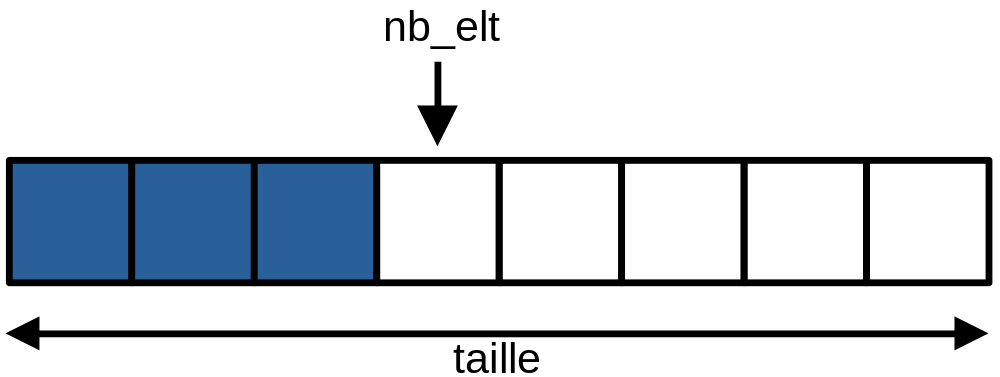
\includegraphics[scale=0.3]{lecon/05-piles_files/piles_tableau.png}
\\

\begin{principe}
	Pour cela, on utilise un indice \texttt{nb\_elt} qui nous indiquera à quelle case du tableau correspond le sommet de la pile, les cases précédentes du tableau contenant les autres éléments empilés.
\end{principe}

\begin{impl}
	On doit soit alors utiliser un tableau de taille fixe (et donc connaître à l'avance le nombre max d'éléments dans la pile)
\end{impl}

\chapter{Implémentations et applications des ensembles et des dictionnaires}
\label{L6}
\dev{Emile Martinez}{}{}{}

\section{Dictionnaire : type abstraits et motivation}


\begin{definition}[Dictionnaire]
	Soit $X$ un ensemble d’éléments appelés valeurs, et $K$ un ensemble d’éléments appelés clés. Un dictionnaire $D$ est une structure de données abstraites ayant les trois opérations :
	
	— $\texttt{Inserer}(D,k,x)$ : insère le couple $(k, x)$ dans $D$, en écrasant un éventuel couple $(k, x')$ préexistant.
	
	— $\texttt{Recherche}(D,k)$ : renvoie la valeur de $x$ telle que $(k, x)$ est dans $D$, si elle existe (peut renvoyer une valeur pas dans $X$ sinon)
	
	— $\texttt{Supprime}(D,k)$ supprime un éventuel couple $(k, x)$ présent dans $D$.
\end{definition} 

\begin{example}
	annuaire téléphonique : les clefs sont les noms des personnes, les valeurs leurs numéros de téléphone
\end{example}

\begin{rem}
	Les dictionnaires sont aussi appelés tableaux associatifs
\end{rem}

\begin{appl}
	Si on a une base de données de personnes, identifiés par un pseudonyme, on peut stocker leur informations dans un dictionnaire.
\end{appl}

\begin{rem}
	C'est ce qui se passe dans une base de données
\end{rem}

\begin{impl}[naive]
	On pourrait stocker tous les éléments dans une liste, sans ordre particulier
\end{impl}

\begin{exercise}
	Implémenter alors les fonctions de bases. Quelles sont leur complexité ?
\end{exercise}

\section{Implémentation}

\subsection{Par des arbres}

\subsubsection{Arbres binaires de recherche (ABR)}

\begin{definition}[ABR]
	Un arbre binaire de recherche (ABR) est un arbre binaire dont les éléments sont munis d'un ordre total et où, pour chaque sous-arbre $N(g, x, d)$, l'élément $x$ est supérieur à tous les éléments de $g$ et inférieur à tous les éléments de $d$.
\end{definition}

\begin{impl}
	On peut implémenter un dictionnaire à l'aide d'un ABR à condition que l'ensemble des clefs soit muni d'un ordre total (On insère les couples (clé, valeur) et l'ordre est sur les valeurs)
\end{impl}

\begin{example} Deux implémentations du même ABR :\\
	\begin{minipage}{0.5\linewidth}
		\begin{tikzpicture}[-, node distance=2cm]
			\node[state] (q0) {10};
			\node[state, below left of = q0] (q1) {8};
			\node[state, below left of = q1] (q2) {5};
			\node[state, below left of = q2] (q3) {3};
			
			\draw (q0) edge[] node{} (q1);
			\draw (q1) edge[] node{} (q2);
			\draw (q2) edge[] node{} (q3);
			
		\end{tikzpicture}
	\end{minipage}\begin{minipage}{0.5\linewidth}
		\begin{tikzpicture}[-, node distance=2cm]
			\node[state] (q0) {5};
			\node[state, below left of = q0] (q1) {3};
			\node[state, below right of = q0] (q2) {10};
			\node[state, below left of = q2] (q3) {8};
			
			\draw (q0) edge[] node{} (q1);
			\draw (q0) edge[] node{} (q2);
			\draw (q2) edge[] node{} (q3);
			
		\end{tikzpicture}
	\end{minipage}
\end{example}

\paragraph{Insertion} Dans un ABR, on insère un élément $x$ en descendant depuis la racine, en prenant le fils gauche ou le fils droit selon si $x$ est plus petit ou plus grand que la racine courante, et en créant un nouveau nœud étiqueté par $x$ lorsque l’on ne peut plus avancer.
	
\paragraph{Recherche} Elle se fait de manière analogue

\paragraph{Suppression} Lorsque le nœud est une feuille ou si le nœud n’a qu’un enfant, alors la transformation est simple. Par contre, si le nœud possède deux enfants, alors il faut retirer le minimum du sous-arbre droit (ou le maximum du sous-arbre gauche) pour le remplacer.

\begin{exercise}
	Implémentation des ABR en OCamL
\end{exercise}

\begin{proposition}
	Soit $\mathcal A$ un ABR à $n$ nœuds et de hauteur $h$. La recherche, l’insertion et la suppression	se font dans le pire cas en $O(h)$ comparaisons. Or un ABR peut être déséquilibré : la hauteur est alors en $O(n)$
\end{proposition}

\subsubsection{Arbres rouge-noir (ARN)}

\begin{definition}
	 Un arbre rouge noir (ARN) est un ABR où chaque nœud porte une couleur rouge ou noir, et qui vérifie les deux propriétés suivantes : \begin{itemize}
		\item la racine est noire 
		\item les potentiels fils d'un nœud rouge sont noirs
		\item pour chaque nœud, tous les chemins menant de ce nœud à une feuille ont le même nombre de nœuds noirs. 
	\end{itemize}
\end{definition}

\begin{proposition}
	\label{06-equilibre}
	Les ARN sont équilibrés ($h = O(\log n)$)
\end{proposition}

\begin{corollary}
	Dans un ARN, on peut effectuer les opérations d'insertion, de recherche et de suppression en $O(h)$, ie $O(\log n)$. 
\end{corollary}

\paragraph{Developpement} Preuve de la propriété \ref{06-equilibre} et présentation de l'insertion dans un ARN

\subsection{Tables de hachage}

\begin{idee}
	Le but ici va être de stocker nos données dans un tableau (d'où le nom tableau associatif). Cela se fait donc en deux étapes : \begin{itemize}
		\item Associer à notre données un nombre (pas trop grand) (appelé hachage) par une fonction appelée fonction de hachage.
		\item Avoir un tableau avec une case par hachage possible, où l'on stocke la donnée
	\end{itemize}
\end{idee}

\subsubsection{Fonction de hachage}

\begin{definition}
	Une fonction de hachage est une fonction $h : K \to \llbracket 0, m-1 \rrbracket$ (avec $m << |K|$)
\end{definition}

\begin{proposition}
	Une fonction de hachage a la propriété du hachage parfait si pour $x \neq y \in K$, $\mathbb P(h(x) = h(y)) = \dfrac{1}{m}$
\end{proposition}

\begin{rem}
	Le hachage parfait veut dire que les valeurs de hachage sont comme pris au hasard dans $\llbracket 0, m-1\rrbracket$. Néanmoins, comme on veut que $h(x)$ vaille toujours la même chose, on ne prend pas de fonctions aléatoires.
\end{rem}

\begin{example}
	On choisit un flottant A. On interprète les bits de données de la structure comme un entier x (en les collant). On prend alors $h(d) = \lfloor A*x \rfloor \mod m$
\end{example}

\subsubsection{Table de hachage}

Il y a trois étapes dans le stockage dans un tableau: \begin{enumerate}
	\item Hacher la valeur et la mettre dans à sa case dans le tableau
	\item Si la case était déjà occupée (collision), stocker la donnée dans une structure annexe
	\item Si le tableau est trop plein, augmenter m (et donc recopier toutes les données).
\end{enumerate}

\begin{example} Schéma où la structure annexe est une liste chaînée pour chaque case\\
	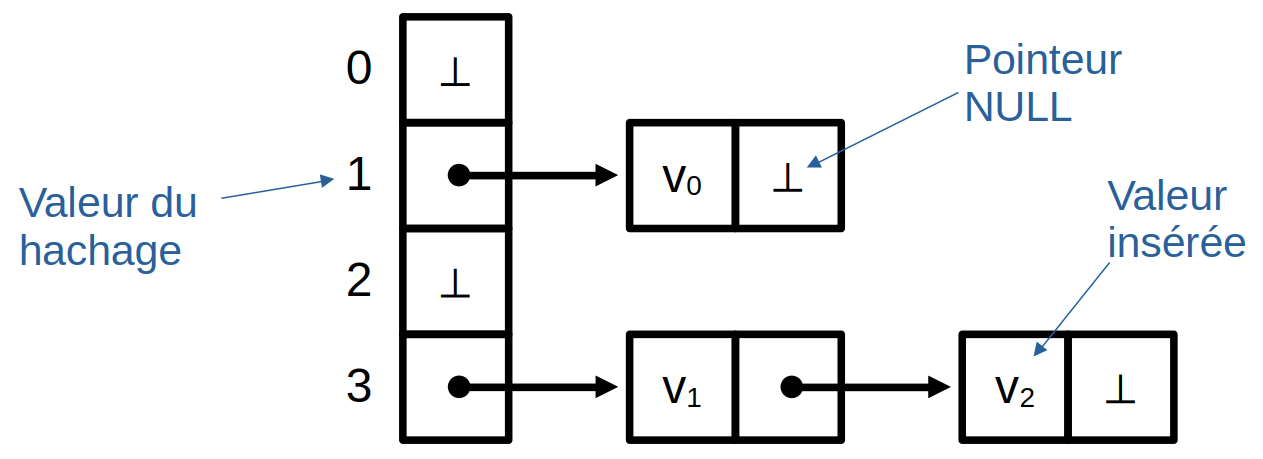
\includegraphics[width = 0.7\linewidth]{lecon/06-ensembles_et_dictionnaires/table_hachage.png}
\end{example}

\begin{com}
	Si on a la place on peut ecrire la remarque, sinon le dire à l'oral que si les abr nécessite un ordre total, la table de hachage nécessite de sérialiser ou de donner directement le hachage
\end{com}

\begin{com}
	Normalement là on pourrait parler de compexité, mais on considère que le tableau \ref{06-tab} suffit.
\end{com}

\section{Ensembles}

\begin{definition}
	Un ensemble est un dictionnaire dans lequel il n'y a pas de clefs. La fonction recherche renvoie donc un booléen qui indique la présence ou non de l'élément. 
\end{definition}

\begin{rem}
	On déduit alors de l'implémentation des dictionnaires, l'implémentation des ensembles
\end{rem}

\begin{com}
	Cette remarque justifie que l'on parle si brièvement des ensembles, et si tard dans la leçon. Beaucoup des choses sur les ensembles se déduisant de celles des dictionnaires
\end{com}

\begin{idee}
	Comme ce sont des ensembles on pourrait également vouloir des opérations ensemblistes comme l'union, l'intersection, etc...
\end{idee}

\begin{impl}
	On peut faire ces opérations sur les structures précédentes en les parcourant (pour l'union, on insère tous les éléments de l'un dans l'autre par exemple)
\end{impl}

\begin{rem}
	Ces opérations réhabilite l'idée de la liste triée
\end{rem}

Récapitulatif des complexités :\\


\begin{tabular}{|l|c|c|c|c|c|}
	\hline \label{06-tab} Structure & Insertion & Suppression & Recherche & union & intersection\\
	\hline liste & $O(n)$ & $O(n)$ & $O(n)$ & $O(n\times m)$ & $O(n \times m)$ \\
	\hline liste triée & $O(n)$ & $O(n)$ & $\log n$ & $O(n+m)$ & $O(n+m)$\\
	\hline ARN & $O(\log n)$ & $O(\log n)$ & $O(\log n)$ & $O(n+m)\log(n+m)$ & $O(\min(n,m) \log(\max(n,m)))$\\
	\hline Table de  & $O(n)$ & $O(n)$ & $O(n)$ & $O(n\times m)$ & $O(n \times m)$ \\
	hachage & $O(1)$ moy. & $O(1)$ moy. & $O(1)$ moy. & $O(n+m)$ moy. & $O(\min(n,m))$ moy. \\ \hline 
\end{tabular}

\begin{exercise}
	Choisir des implémentations en C et les comparer. Si l'on traite les listes triées, ouverture sur les skip listes
\end{exercise}

\section{Application}

\subsection{Dictionnaire d'adjacence}

Soit $G=(S, A)$ un graphe. (où $S = \llbracket 1, n \rrbracket$)\\

On peut représenter $G$ par un tableau de dictionnaire $D$ tq $D[u]$ est un dictionnaire contenant les voisins de $u$\\

\textbf{intérêts :} On a les avantages de la matrice d'adjacence (on detecte rapidement si il y a une arête) et des listes d'adjacence (stockage en |A| et obtention de tous les voisins linéairement).\\

\begin{example}
	Sur un graphe de personnes se connaissant, on sait si A connait B rapidement, mais on n'a pas à stocker tous les false des couples de personnes en se connaissant pas.
\end{example}

\subsection{Mémoïsation}
Supposons que l'on ait une fonction du type
\begin{lstlisting}
fonction (f_args):
    corps de f
    return x
\end{lstlisting}

Il se peut que l'on ait beaucoup d'appels à \texttt f sur les mêmes arguments, comme des fonctions récurisves en programmation dynamique. En s'inspirant de cette dernière, on peut alors ne faire qu'une fois les appels sur chaque argument grâce à un dictionnaire :

\begin{lstlisting}
fonction f(args):
    Si args est dans dictionnaire:
        renvoyer dictionnaire[args]
    Sinon:
        corps de f
    dictionnaire[args] = x
    renvoyer x
\end{lstlisting}

\subsection{Autres applications}

\begin{com}
	On peut dire à l'oral que en gros, utiliser un dictionnaire est un peu équivalent à $f : K \to \llbracket 1, K \rrbracket$. (c'est plus que simplement le fait logique que, par un tableau classique, c'est équivalent)
\end{com}

Les dictionnaires et les ensembles servent dès que l'on veut accéder rapidement à un élément dont la structure n'est pas un entier.

\begin{example}
	En algorithmique du texte, pour associer des valeurs à des chaînes de caractère (Huffman, Boyer-Moore)
\end{example}

\begin{example}
	Quand on fait un parcours de graphe dont les sommets ne sont pas $\llbracket 1, n \rrbracket$ on peut utiliser un ensemble pour savoir quels éléments on a déjà parcouru.
\end{example}

\begin{com}
	On peut soit insister à l'oral sur cet exemple, soit en faire une sous partie, du fait que c'est une application pour les ensembles
\end{com}

Mais on peut les retrouver également dans beaucoup de domaines comme en bases de données, et dès que l'on manipule un nombre faible de valeur comparés à l'ensemble des valeurs possibles.

\textbf{Développement :} Amélioration du tri par comptage par l'usage de dictionnaires.

\chapter{Accessibilité et chemins dans un graphe. Applications}
\label{L7}
\dev{Emile Martinez}{}

\begin{com}
	Les applications sont éparpillées tout le long de la leçon, et relativement peu développer, donc il peut-être rentable des les souligner pendant la défense de plan.
\end{com}

\section{Definition}

\begin{definition}[chemin]
	Dans un graphe orienté $G$ (resp. non orienté) on appelle chemin de longueur $\lambda$ une suite de $(\lambda + 1)$ sommets $(s_0, \, s_1, \,\dots, \, s_\lambda)$
\end{definition}

\begin{rem}
	Par convention, on dit qu’il y a un chemin de longueur 0 de tout sommet vers lui-même.
\end{rem}

\begin{rem}
	Dans un graphe non-orienté, les chemins sont aussi appelés chaînes.
\end{rem}

\begin{appl}
	Dans un graphe de flot de contrôle, le critère tous les chemins consiste à trouver des tests qui font tous les chemins possibles du graphe
\end{appl}

\begin{com}
	Une première application, dont on ne parle pas beaucoup plus parce que ca a pas grand chose a voir. Donc les chemins servent là, mais la théorie derrière n'est pas intéressante par la théorie des graphes. Illustre simplement la diversité de l'utilisation des graphes.
\end{com}

\begin{com}
	On peut mentionner que ca fait déjà une première application
\end{com}

\begin{definition}[chemin élémentaire]
	Un chemin est dit élémentaire s’il ne contient pas plusieurs fois le même sommet.
\end{definition}

\begin{com}
	Par manque de place, cette définition peut être enlevé
\end{com}

\begin{definition}[circuit/cycle]
	Dans un graphe orienté (resp. non orienté), un chemin $(s_0, \, \dots, \, s_\lambda)$ dont les $\lambda$ arcs (resp. arêtes) sont distincts deux à deux et tels que $s_0 = s_\lambda$ , est un circuit (resp. un cycle).
\end{definition}

\begin{example}
	On dit qu'un circuit est hamiltonien si il passe par tous les sommets une et une seule fois. Décider de l'existence d'un tel circuit dans un graphe est NP-complet (i.e. dur)
\end{example}

\begin{exercise}
	On dit qu’un graphe non orienté est Eulérien s’il existe un cycle passant par chaque arête exactement une fois. Montrer qu’un graphe est eulérien si et seulement si tous ses sommets sont de degré pair.
\end{exercise}

\begin{com}
	Ces deux choses là peuvent être présenter comme des formes d'applications, du moins d'application des définitions (il semble important que la NP-complétude de quelque chose soit mentionné dans cette leçon)
\end{com}

\begin{definition}[accessibilité]
	Étant donné un graphe $G$ (orienté ou non) et deux sommets $s$ et $t$, on dit que $t$ est accessible depuis $s$ s’il existe un chemin allant de $s$ à $t$ dans $G$.
\end{definition}

\section{Accessibilité}

\subsection{Tri topologique}

\begin{definition}[tri topologique]
	Étant donné un graphe orienté $G = (S,A)$, on dit que $\sigma : S \to \llbracket 1,  |S| \rrbracket$ est un tri topologique si $(s,t) \in A \implies \sigma(s) < \sigma(t)$
\end{definition}

\begin{corollary}
	Soit $\sigma$ un tri topologique sur $G$. Pour $s, t \in S$, si il existe un chemin de $s$ à $t$, alors $\sigma(s) \leq \sigma(t)$
\end{corollary}

\begin{proposition}
	$G$ est acyclique si et seulement si $G$ admet un tri topologique.
\end{proposition}

\begin{proof}[pour le sens direct]
	On montre par l'absurde par récurrence qu'un graphe acyclique a un sommet source.\\
	On montre par récurrence la proposition sur $|S|$
\end{proof}

\begin{algo}Construction d'un tri topologique
	\begin{itemize}[label=$\bullet$]
		\item Créer une pile vide
		\item Faire un parcours en largeur postfixe de G en appliquant la fonction empile
		\item Renvoyer la pile
	\end{itemize}
\end{algo}

\begin{appl}
	Ordonnancement de tâches
\end{appl}

\begin{definition}
	Soit $T=\{ t_1, \, \dots, \, t_n \}$ un ensemble de tâches d'un ordinateur et $C = T^2$ un ensemble de contraintes $((t_i, t_j) \in C$ veut dire que $t_i$ doit être fait avant $t_j$). Un ordonnancement de ces tâches est un ordre d'éxécution de ces tâches.
\end{definition}

\begin{proposition}
	On peut trouver un ordonnancement en temps linéaire
\end{proposition}

\begin{proof}
	On prend le graphe $(T, C)$ est on fait un tri topologique.
\end{proof}

\subsection{Connexité}

\begin{proposition}
	La relation «il existe un chemin de $s$ à $t$ et de $t$ à $s$» est une relation d'équivalence.
\end{proposition}

\begin{exercise}
	Montrer que le graphe quotienté par cette relation d'équivalence est acyclique
\end{exercise}

\begin{com}
	Ici on introduit le DAG des classes des composantes (fortement) connexes. On peut néanmoins dire que suivant le niveau de la classe, il est très probable que le terme quotienté ne soit pas maitrisé. Donc la on le met par concision, au cas où il aurait déjà était vu en maths (hors programme en maths), mais en vrai on pourrait périphraser et faire des définitions. De plus la c'est un plan, donc on dit ce qu'on ferait dans l'exercice, pas tout l'énoncé rigoureux.
\end{com}

\begin{definition}
	Dans un graphe non orienté (resp. orienté), les classes d'équivalence de cette relation sont appelés composantes connexes (resp. fortement connexes).\\
	Si il n'y a qu'une seul classe, le graphe est dit connexe (resp. fortement connexe)
\end{definition}


\begin{com}
	On prend ca comme déf et non pas la propriété suivantes en ayant défini connexe comme un chemin de tous le monde à tout le monde, pour avoir une définition plus explicites et naturelles que de passer par la maximalité. Néanmoins, cela nécessite l'abstraction de la classe d'équivalence (vue en maths). Si la classe est faible, on peut faire tout ca plus avec les mains.
\end{com}

\begin{exercise}
	Dans un graphe connexe, deux chemins élémentaires maximaux ont un nœud en commun.
\end{exercise}

\begin{proposition}
	Une composante connexe (resp. fortement connexe) est un sous-graphe connexe (resp. fortement connexe) maximal.
\end{proposition}

\begin{algo} \enspace\\
	\begin{algorithm}[H]
		\Tq{un sommet n'est pas visité}{
		    Créer une nouvelle composante connexe\\
			Parcourir le graphe des sommets non visités depuis un sommet v non visité en ajoutant a la composante tous les sommets que l'on croise
		}
		\caption{Calcul des composantes connexes (cas non orienté)}
	\end{algorithm}
\end{algo}

Pour les composantes fortement connexes, il faudra plus qu'un simple parcours.

\begin{algo}\enspace \\
	\begin{algorithm}[H]
		\caption{Algorithme de Kosaraju}
		Appliquer l'algorithme de construction d'un tri topologique (meme si le graphe a des cycles)\\
		Prendre $G^T$ le graphe transposé de $G$ (i.e., $(u,v)$ devient $(v,u)$)
		\Pour{i allant de 1 à n}{
			Si $\sigma(i)$ n'a pas déjà été visité\\
			Créer une nouvelle composante fortement connexe\\
			Visiter $G^T$ depuis $\sigma(i)$ en ajoutant les sommets visités non encore attribués\\
		}
	\end{algorithm}
\end{algo}

\begin{proposition}
	Cet algorithme construit les composantes fortement connexes en temps linéaire
\end{proposition}

\begin{definition}
	Le problème 2-SAT est le problème de savoir si étant donné $n$ variables $x_1, \,\dots ,\, x_n$ et $p$ clauses $C_1, \,\dots ,\, C_p$ de taille 2 sur $x_1,\, \dots, \, x_n$, $\varphi = \bigwedge\limits_{i=1}^p C_i$ est satisfiable
\end{definition}

\textbf{Developpement :} Résolution en temps linéaire de 2-SAT.

\section{Plus court chemin}

\begin{definition}[graphe pondéré]
	Un graphe pondéré est un graphe $G = (S, A)$ muni d’une fonction de poids $w : A \to Z$.\\
	Le poids d’un chemin est alors défini comme la somme des poids des arêtes qui le compose.
\end{definition}

\begin{rem}
	On peut étendre $w$ à $S^2$ en posant $w(u, v) = +\infty$ lorsque $(u, v) \notin A$.
\end{rem}

\begin{definition}
	Dans un graphe $G$, un plus court chemin (pcc) de $u$ à $v$ ($u,v\in S$) est un chemin de poids minimal de $u$ à $v$
\end{definition}

\begin{rem}
	Si les poids sont unitaires, on peut trouver le pcc entre deux sommets $u$ et $v$ en faisant un parcours en largeur depuis $u$.
\end{rem}

\begin{com}
	On considère les parcours déjà vu (servant dans bien d'autres contextes que les chemins dans les graphes). Ici on fait simplement le lien, et on illustre la notion. On pourrait également le faire sur un exemple au tableau, et essayer de le faire devnier aux élèves (lien entre différentes parties du cours)
\end{com}

\subsection{D'un sommet à tous les autres}

Lorsque la fonction de poids est à valeur dans $\N$, on peut utiliser l'algorithme de Dijkstra.

\begin{algo} 
	\enspace \\
	\begin{algorithm}[H]
		\caption{$dijkstra(G, S)$}
		$distance \gets $ tableau de taille $|S|$ initialisé à $+\infty$\\
		$distance[s] \gets 0$\\	
		$F \gets FilePriorite()$\\
		$Inserer(F, s, 0)$\\
		\Tq{$\neg estVide(F )$}{
			$u, du \gets ExtraireMin(F)$\\
			\Pour{$v \in N(u)$}{
				$d \gets du + w(u, v)$\\
				
				\Si{$d < distance[v]$}{
					\eSi{$distance[v] = +\infty$}{
						$Inserer(F ,v,d)$
					}{
						$DiminuerPriorite(F ,v,d)$\\
						$distance[v] \gets d$
					}
				}
			}
		}
		\Retour $distance$
	\end{algorithm}
\end{algo}


\begin{proposition}
	L’algorithme de Dijkstra réalise au plus $|S|$ appels à $Inserer$ et $ExtraireMin$, et $|A|$ appels à $DiminuerPriorite$.\\
	Donc avec un tas min, on obtient $O(|A| \times \log |S|)$
\end{proposition}

\begin{rem}
	Si la structure d'entrée est une matrice d'adjacence, on peut faire l'algorithme en $O(n^2)$ sans structure particulière pour $F$.
\end{rem}

\begin{rem}
	Lorsque la fonction de poids est à valeur dans $\mathbb Z$ et que le graphe ne contient aucun circuit absorbant, on peut utiliser l'algorithme de Bellman-Ford.
\end{rem}

\begin{appl}
	Détection des cycles absorbants.
\end{appl}

\begin{rem}
	Si l'on souhaite seulement le plus court chemin entre deux points, on peut utiliser l'algorithme A* (Dijkstra + heuristique du chemin restant).
\end{rem}

\subsection{De tous les sommets à tous les sommets}

Lorsque le graphe ne contient aucun cycle absorbant, l'algorithme de Floyd Warshall calcule les plus courts chemins entre toute paire de sommets de $S=\{1, \, \dots , \,n\}$ par programmation dynamique. \begin{itemize}[label=$\star$]
	\item \textbf{Sous-problèmes :} $d^{(k)(i,j)}$ la distance du pcc de $i$ à $j$ avec seulement $\llbracket 1, k \rrbracket$ comme sommets intermédiaires
	\item \textbf{Relation de récurrence}
	$$ \begin{array}{l}
		d^{(0)}(i,j) = w(i,j)\\
		d^{(k+1)}(i,j) = \min\left(d^{(k)}(i,j), \enspace d^{(k)}(i,k) + d^{(k)}(k, j)\right)
	\end{array} $$
	\item \textbf{Résolution :} On résout sur $S^2$ à $k$ croissant
\end{itemize}

\begin{proposition}
	Floyd Warshall est en $O(n^3)$
\end{proposition}

\begin{rem}
	Si les poids sont positifs, appliquer dijkstra à chaque sommet nous donne $O(n \times |A| \times \log n)$
\end{rem}

\begin{rem}
	Cette algorithme utilise une matrice d'adjacence (algorithme centralisé)
\end{rem}

\begin{algo}
	Si on a des listes d'adjacence (algorithme décentralisé/distribué), on peut utiliser l'algorithme de Bellman Ford
\end{algo}

\begin{appl}
	Routage des paquets d'un réseau par le protocole IP avec l'algorithme de Bellman Ford.
\end{appl}

\noindent \textbf{Developpement :} Presentation et terminaison de l'algorithme de Bellamn Ford.


\begin{com}
	On a fait une leçon sur les graphes, sans aucun dessin de graphes. En vrai, il pourrait y en avoir sur des exemples, et puis les schémas ne sont pas absolument necessaires pour illustrer la plupart des concepts, dont surtout la formalisation est imporante (la def d'un chemin est explicite).
\end{com}




\chapter{Algorithme de tri. Exemple, Complexité et Applications}
\label{L8}
\dev{Emile Martinez}{}

\section{Introduction}

\begin{definition}
	Un algorithme de tri prend en entrée un liste d'éléments $E$ muni d'un ordre total $\leq$ ( mais dont on peut se passer de l'antisymétrie) et renvoie o=une liste $S$ telle que : \begin{enumerate}
		\item elle contient exactement les éléments de $E$
		\item les éléments de $S$ apparaissent dans l'ordre croissant
	\end{enumerate}
\end{definition}

\begin{appl}
	Pourquoi trier ? Cela permet de simplifier des opérations (min, max, recherche, etc...)
\end{appl}

\begin{exercise}
	Chercher à la main un mot dans une liste triée et non triée.
\end{exercise}

\begin{com}
	\label{08-activite}
	On peut faire cet exercice en seconde. Avec éventuellement le fait de comparer deux listes de mots. Tout ca pour voir l'intérêt du tri. Ensuite on peut leur demander comment faire pour trier, permettant de faire émerger des algorithmes sans le formalismes nécessaires. Et suivant le format des mots, on obtiendra probablement des choses différentes (une liste écrit sur un papier -> tri par sélection, des cartes avec les mots -> tri par insertion, tri a bulle, voir même du tri par paquet).
	
	Ainsi on peut faire de l'informatique sans l'écueil de  l'apprentissage de la syntaxe python qui bloque beaucoup d'élèves.
\end{com}

\begin{definition}[Propriétés des tris]
	\begin{itemize}[label=$\bullet$]
		\item en place : Utilise $O(1)$ espace en plus de l'espace des données d'entrées
		\item stable : Si $E[i] \leq E[j]$ et si $E[j] \leq E[i]$, avec $i < j$, dans $S$, $E[i]$ apparaîtra avant $E[j]$
		\item en ligne : on peut trier les données même si elles arrivent au fur et à mesure
		\item parallélisable : on peut diviser le travail sur plusieurs fils.
	\end{itemize}
\end{definition}

\section{Tri quadratiques}

\subsection{Tri par sélection}

\begin{minipage}{0.5\linewidth}
	\begin{algorithm}[H]
		\caption{$Tri\_par\_selection(E)$}
		$S \gets [\,]$\\
		\Pour{$i$ allant de $1$ à $|E|$}{
			Extraire $mini$, le minimum de $E$\\
			Ajouter $mini$ à la fin de $S$
		}
		\Retour $S$
	\end{algorithm}
\end{minipage} \begin{minipage}{0.5\linewidth}
	\begin{example} \normalfont
		\begin{center}$E = [4, \, 3, \, 6, \, 1]$\\
			\begin{tabular}{|c|c|c|c|}
				\hline $i$ & $E$ & $m$ & $S$\\
				\hline $\times$ & [4, 3, 6, 1] & $\times$ & []\\
				\hline 0 & [4, 3, 6] & 1 & [1]\\
				\hline 1 & [4, 6] & 3 & [1, 3]\\
				\hline 2 & [6] & 4 & [1, 3, 4]\\
				\hline 3 & [] & 6 & [1, 3, 4, 6]\\
				\hline
			\end{tabular}\\
			$S = [1, \, 3, \, 4, \, 6]$
		\end{center}
	\end{example}
\end{minipage}

\begin{com}
	Cet exemple peut être remplacer par simplement : «Exemple : mettre un exemple d'execution de l'algorithme» si on manque de place
\end{com}

\begin{proposition}
	\enspace\\
	\begin{itemize}[label=$\star$]
		\item Terminaison : l'algorithme n'utilise que des boucles bornées
		\item Correction : Invariant de boucle «$S$ est trié et contient les $i$ plus petits de $E$»
		\item Cout : environ $|E|^2$
	\end{itemize}
\end{proposition}

\begin{proposition}
	Le tri par sélection est stable (si on extrait le premier min) mais ni en ligne, ni en place, ni facilement parallélisable
\end{proposition}

\begin{exercise}
	Réécrire le tri pour qu'il soit en place. Qu'advient-il de la stabilité ?
\end{exercise}

\subsection{Tri par insertion}

\begin{algorithm}[H]
	\caption{$Tri\_par\_insertion$}
	\Pour{$i$ allant de $0$ à $|E|-1$}{
		$v \gets E[i]$\\
		$j \gets i-1$\\
		\Tq{$j > 0$ et $E[j] > E[j+1]$}{
			Échanger $E[j]$ et $E[i]$\\
			$j \gets j-1$\\
		}
	}
	\Retour{E}
	\label{08-inser}
\end{algorithm}

\begin{proposition}
	L'algorithme \ref{08-inser} est stable, en place et en ligne.
\end{proposition}

\begin{rem}
	Il est difficilement parallélisable
\end{rem}

\begin{exercise}
	Quel est la complexité de cet algorithme
\end{exercise}

\subsection{Recherche Dichotomique}

\begin{algorithm}[H]
	\caption{$Recherche\_dichotomique(E, x)$}
	\eSi{$|E| = 0$}
	{
		\Retour{Faux}
	}
	{
		$a \gets 0, \, b \gets |E|-1, \, m \gets \left\lfloor \dfrac{a+b}{2} \right\rfloor$\\
		\Tq{$E[m] \neq x$ et $(b-a)>0$}{
			\eSi{$E[m] < x$}
				{$a \gets m+1$}
				{$b \gets m-1$}
			$m \gets \left\lfloor \dfrac{a+b}{2} \right\rfloor$
		}
		\eSi{$E[m] = x$}
			{\Retour{Vrai}}
			{\Retour{Faux}}
	}
\end{algorithm}

\noindent\textbf{Terminaison :} variant de boucle : «$b-a$»\\
\textbf{Correction :} invariant de boucle : «Si $x$ est dans $E$ alors son indice est entre $a$ et $b$»\\
\textbf{Cout :} nombre de bit de $|E|$

\begin{impl}
	Implémentation en Python et comparaison avec la recherche linéaire
\end{impl}

\begin{exercise}
	Écrire une version récursive de l'algorithme
\end{exercise}

\section{Tri efficace}

\subsection{Tri fusion}

\begin{definition}
	L'algorithme de tri fusion est un algorithme de tri qui repose sur deux opérations : \begin{itemize}
		\item $partitionner(L)$ : coupe $L$ en deux listes de taille équivalente $L_1$, $L_2$
		\item $fusion(L_1, L_2)$ : avec $L_1$ et $L_2$ deux listes triées, renvoie $L3$ la liste triée contenant tous les éléments de $L_1$ et $L_2$.
	\end{itemize}
\end{definition}

\begin{algorithm}[H]
	\caption{fusion($L_1$, $L_2$)}
	$res \gets []$\\
	$i,j \gets 0$\\
	\Tq{
		$i < |L_1|$	et $j < |L_2|$
	}{
		\eSi{$L_1[i] < L_2[j]$}{
			$res$.ajouter($L_1[i]$) \\
			$i \gets i + 1$
		}{
			$res$.ajouter($L_2[j]$) \\
			$j \gets j + 1$
		}
	}
	Ajouter le reste de $L_1$ et de $L_2$ à $res$\\
	\Retour{$res$}
\end{algorithm}

\begin{algorithm}[H]
	\caption{tri\_fusion($L$)}
	$n \gets |L|$\\
	\Si{$n\leq 1$}{
		\Retour{$L$}
	}
	$L_1, L_2 \gets$ partionner($L$)\\
	\Retour{fusion( tri\_fusion($L_1$), tri\_fusion($L_2$) )}
\end{algorithm}

\textbf{Developpement :} Correction totale du tri fusion

\begin{proposition}
	Ce tri est stable mais pas en place. Parallélisable mais pas en ligne.
\end{proposition}

\textbf{Complexité :} $C(n) = 2\times C(\frac{n}{2})$ donc $C(n) = O(n \times \log n)$

\subsection{Tri rapide}

\begin{idee}
	Choisir un élément appelé pivot et mettre à gauche tous les éléments plus petit, à droite tous les plus grands, puis à trier cette partie à droite et à gauche.
\end{idee}

\begin{algorithm}
	\caption{$tri\_rapide(L, debut, fin)$}
	\Si{$debut \geq fin -1$}
		{\Retour{$L$}}	
	$pivot \gets L[0]$\\	
	$i \gets debut$\\
	$j \gets fin$\\
	\Tq{$i < j$}
	{
		\eSi{$L[i+1] \leq pivot$}
		{
			échanger $L[i+1]$ et $L[i]$\\
			$i \gets i+1$
		}{		
			échanger $L[i+1]$ et $L[j]$\\
			$j \gets j - 1$
		}
	
		$tri\_rapide(L, debut, i-1)$\\	
		$tri\_rapide(L, i+1, fin)$\\
	}
\end{algorithm}

\begin{com}
	Par manque de place, on peut remplacer l'écriture de cet algorithme par un dessin expliquant l'idée, et mettre son écriture en exo
\end{com}

\begin{proposition}[Complexité]
	\begin{itemize}
		\item pire des cas : $O(n^2)$
		\item meilleur cas : $O(n\log n)$
		\item cas moyen avec pivot aléatoire : $O(n\log n)$
		\item pire cas avec pivot astucieux : $O(n\log n)$
	\end{itemize}
\end{proposition}

\begin{proposition}
	Ce tri est en place, non stable, non en ligne mais parallélisable
\end{proposition}

\begin{com}
	On peut éventuellement mentionner que dans beaucoup d'implémentation, pour le pivot on prend quelques valeurs (exemple 5) et on prend la médiane de ces valeurs là (ainsi on est quasiment jamais dans le pire cas et sans devoir calculé la médiane). Mais avec l'avantage de rester en place
\end{com}

\begin{com}
	Pour le caractère en place, il faut discuter de la pile d'appel. A priori, l'espace supplémentaire utilisé est en $O(\log n)$ (voir $O((\log n)^2$ si on considère le stockage des indices mais là on part un peu trop loin)) et non $O(1)$, mais on s'en contente souvent.
\end{com}

\begin{exercise}
	Écrire une version stable de ce tri. Préserve-t-on le caractère en place.
\end{exercise}

\subsection{Tri par tas}

\begin{algorithm}[H]
	\caption{$tri\_tas(L)$}
	Insérer les éléments de $L$ dans un tas initialement vide\\
	Extraire successivement l'élément minimum du tas.
\end{algorithm}

\begin{exercise}
	Quelles propriétés vérifie ce tri ?
\end{exercise}

\subsection{Minoration de la complexité du tri}

\begin{proposition}
	On ne peut pas trier n éléments avec une complexité inférieure à $n-1$
\end{proposition}

\begin{proposition}
	Un algorithme de tri par comparaison aura une complexité pire cas au mieux $O(n \log(n))$
\end{proposition}

\begin{proof}
	S'intéresser à l'arbre des chemins que prend l'algorithme en fonction du résultat des comparaisons.
\end{proof}

\begin{rem}
	Si on ne trie pas par comparaison, on peut avoir des complexités plus faibles. Par exemple, si E ne contient que des entiers entre 0 et 9, on peut simplement compter le nombre de 0 et de 9 puis reconstruire là dessus le tableau trié.
\end{rem}

\textbf{Développement :} Amélioration du tri par comptage avec des dictionnaires

\section{Application}

\subsection{Algorithmes gloutons}

\begin{definition}
	Un algorithme glouton est un algorithme qui résout un problème d'une entrée $E$ de la forme : \begin{itemize}
		\item on trie les éléments de $E$
		\item on construit une solution en les parcourant, sans revenir en arrière
	\end{itemize}
\end{definition}

\begin{example}
	\label{08-gymnase}
	On a $n$ évènements sportifs ayant lieu respectivement entre les dates $d_i$ et $f_i$ ($i \in \N$) ayant chacun besoin d'un gymnase. Comment allouer des gymnases à des évènements pour utiliser le moins possible de gymnase ? \\
	
	Algorithme glouton :\begin{enumerate}
		\item Trié les évènements par $d_i$ croissant (impliquant souvent de trier)
		\item Mettre chaque évènement dans le premier gymnase vide (peut en être un nouveau)
	\end{enumerate}
\end{example}

\begin{proposition}
	Le glouton de l'exemple \ref{08-gymnase} renvoie une solution optiamle (minimisant le nombre de gymnases)
\end{proposition}

\begin{exercise}
	Écrire un algorithme glouton pour le problème de rendu de monnaie
\end{exercise}

\begin{definition}
	Un arbre couvrant minimal d'un graphe pondéré est un sous graphe connexe acyclique de poids minimal
\end{definition}

\begin{algorithm}[H]
	\caption{$kruskal$}
	\Entree{$L$ liste d'arêtes}
	\Sortie{Arbre couvrant de poids minimal}
	Trier $L$\\
	$res \gets []$
	\Pour{$a \in L$}{
		\Si{$\{a\}\cup res$ n'ajoute pas de cycles}{
			$res \gets res \cup \{a\}$
		}
	}
	\Retour{$res$}
\end{algorithm}

\begin{exercise}
	Proposer des algorithmes gloutons pour la coloration de graphe. Sont-ils optimaux ?
\end{exercise}

\subsection{Implémentation des ensembles}

\begin{com}
	Cette partie fait un peu écho à l'activité mentionner dans le commentaire \ref{08-activite}
\end{com}

\begin{proposition}
	On peut implémenter les ensembles par des listes, par des listes triées, par des listes que l'on trie pour l'union et l'intersection. On obtient alors les complexités suivantes :\\ \normalfont \begin{tabular}{|l|c|c|c|c|}
		\hline Structure & Insertion & Suppression & Recherche & union / intersection\\
		\hline liste & $O(n)$ & $O(n)$ & $O(n)$ & $O(n\times m)$ \\
		\hline liste triée & $O(n)$ & $O(n)$ & $\log n$ & $O(n+m)$ \\
		\hline liste avec tri & $O(1)$ & $O(n)$ & $O(n)$ & $O((n+m) \log(\min(n, m)))$ \\
		\hline
	\end{tabular}
\end{proposition}

\begin{exercise}
	Proposer une implémentation mélangeant les listes triées et les listes avec tri ayant de meilleur complexité
\end{exercise}

\begin{com}
	On s'attend ici à ce que on aient d'une part les éléments déjà triés, de l'autre les éléments pas encore, et on ne trie que quand on fait l'union ou l'intersection (ou éventuellement la recherche) en triant les éléments pas encore triés, puis en fusionnant (cf tri fusion) les deux listes.
\end{com}

\chapter{Algorithmique du texte. Exemples et applications.}
\label{L9}
\dev{Emile Martinez}{}

Un auteur envoie son manuscrit à un éditeur. Il commence par compresser le texte. A la réception, l'éditeur compare le manuscrit à d'autres ouvrages pour vérifier qu'il n'y a pas plagiat. Il peut ensuite chercher un motif dans le texte.

\begin{com}
	Cela justifie l'ordre dans lequel on a mis nos parties. De plus, suivant le niveau du cours, on pourrait inaugurer chaque partie en rappelant quelle partie de ce contexte cela concerne. Mais là le niveau (MPI) est un peu élevé pour s'apesentir sur ce genre de choses
\end{com}

\textbf{Notation :} On prend les conventions de slicing de python


\begin{com}
	Il n'y a pas de partie application car souvent les applications sont directes depuis les algorithmes. Ainsi on les dissémine illustrant directement le concept	
\end{com}


\section{Encodage et compression}

\subsection{Encodage par lettre}

\begin{definition}[Algorithme de compresssion]
	Un algorithme de compression sans perte est la donnée d'une fonction $f : \Sigma^* \to \Sigma^*$ injective (il existe un unique décodage). 
\end{definition}

\begin{algo}[Codage préfixe]
	\enspace
	\begin{enumerate}
	\item Prétraitement : On construit un arbre binaire $\mathcal A$ qu’on appelle arbre de Huffman dont les feuilles sont les lettres $c \in \Sigma$.
	
	\item Compression : On code chaque lettre c par une suite de 0 et 1 correspondant au chemin (0 : gauche, 1 : droite) de la racine à la feuille contenant c dans $\mathcal A$.
	
	\item Décompression : On décode une suite de 0 et 1 en parcourant le chemin correspondant dans $\mathcal A$.
	\end{enumerate}
\end{algo}

\begin{algo}[Codage de Huffman]
	\label{09-Huff}
	\normalfont On note $f_a$ la fréquence du caractère $a$ dans le texte et on note $f_{\mathcal A} = \sum\limits_{a \in \mathcal A} f_a$\\
	\begin{algorithm}[H]
		Créer une forêt $\mathcal F$ d'arbres binaires réduits à un noeud $(a, f_a)$\\
		\Tq{$|\mathcal F| > 1$}
		{
			Extraire de $\mathcal F$ les arbres $\mathcal A_1$ et $\mathcal A_2$ de plus petites fréquences \tcp{$f_{\mathcal A_1} <= f_{\mathcal A_2}$ à la racine}
			Insérer un arbre de racine $f_{\mathcal A_1} + f_{\mathcal A_2}$ ayant pour fils $\mathcal A_1$ et $\mathcal A_2$ dans $\mathcal F$
		}
		\Retour{$\mathcal A_H$ tel que $\mathcal F = \left\{\mathcal A_H\right\}$}
	\end{algorithm}
\end{algo}

\begin{com}
	Mentionner à l'oral qu'on ferait le lien avec le fait que c'est un algorithme glouton sur les arbres unifiant ceux de fréquences des lettres agrégés minimal.
\end{com}

\begin{theorem}
	L'arbre construit par le codage de Huffman \ref{09-Huff} minimise la quantité $S = \sum\limits_c\in \Sigma f_c d_c$ où $d_c$ est la profondeur du caractère $c$ dans l'arbre. 
\end{theorem}

\begin{idee}
	Cela revient à dire que l'algorithme de Huffman est optimal parmi les codages préfixes
\end{idee}

\begin{exercise}
	Quelle structure pour $\mathcal F$ dans l'algorithme \ref{09-Huff} ? Quelle complexité alors ?
\end{exercise}

\subsection{Encodage par séquences}

\begin{idee}
	On va associer un code à une séquence de lettres (ou motifs)
\end{idee}

\begin{rem}
	Pour cela, on peut utiliser le codage de Huffman, en prenant comme alphabet les mots apparaissant dans le livre. Mais on peut faire quelque chose de spécifique aux séquences, mais moins spécifiques à un livre (car ici le caractère " " comme délimitateur est arbitraire).
\end{rem}

\begin{com}
	Si on manque de places, on peut faire cette remarque uniquement à l'oral
\end{com}

\begin{idee}
	L'agorithme LZW détermine un codage dans un dictionnaire $d$ au fur et à mesure de la lecture du texte (algorithme online). On va coder certains motifs (groupement de lettres consécutives) présents dans le texte.
\end{idee}

\begin{algo}[Compression par LZW]
	\enspace \\
	\begin{algorithm}[H]
		Initialement, les lettres de $\Sigma$ sont codées par un entier (par ex. avec le code ASCII).\\
		$m \gets ''$\\
		\Tq{il reste du texte $s$ à coder}
		{
			Retirer le plus long préfixe $w$ de $s$ qui soit dans $d$\\
			Ajouter le codage de $w$ à la fin de $m$\\
			$w' \gets w$ concaténé avec la prochaine lettre de $s$\\
			Ajouter un nouveau codage pour $w'$ dans $d$
		}
		\Retour{m}
	\end{algorithm}
\end{algo}

\begin{rem}
	Pour la décompression, il n'est pas nécessaire de transmettre le dictionnaire car on peut le reconstruire à la volée. 
\end{rem}

\begin{appl}
	Le format de fichier .zip compresse un dossier en utilisant (entre autre) les algorithmes de Huffman et LZW. 
\end{appl}

\textbf{Développement :} Présentation de la compression et de la décompression de l'algorithme LZW

\section{Comparaison}

\subsection{Plus longue sous-suite commune (PLSSC)}

\begin{definition}[Problème PLSSC]
	Soit $x, y \in \Sigma^*$. Une plus longue sous-suite commune à $x$ et $y$, noté $PLSSC(x,y)$ est $argmin \left\{k \: \big/ \: \exists i,j : x[i:i+k] = y[j:j+k]\right\}$
\end{definition}

\begin{appl}
	Ce problème correspond au fait de trouver des morceaux d'ADN communs entre deux séquençages.
\end{appl}

\begin{example}
	Pour $x = 'patate'$ et $y = 'frites'$ on a $'te'$
\end{example}

\begin{algo}[Brute force]
	On essaie toutes les séquences possibles $\to$ exponentiel
\end{algo}

\begin{algo}[programmation dynamique]
	\label{09-PLSCC}
	On considère les sous-problèmes  $c_{i,j} = \left| PLSSC(x[:i], y[:j]) \right|$.\\
	On a alors $c_{i,j} = \left\{
	\begin{array}{ll}
		0 & \text{si } i = 0 \text{ ou } j = 0 \\
		c_{i-1, j-1} & \text{si } x[i-1] = y[j-1]\\
		\max(c_{i-1, j}, c_{i, j-1}) & \text{sinon} \\
	\end{array}\right.$
\end{algo}

\begin{proposition}
	L'algorithme \ref{09-PLSCC} calcule $PLSSC(x, y)$ en $O(|x| \times |y|) $
\end{proposition}

\begin{rem}
	Pour obtenir la sous suite, on sauvegarde d'où l'on vient pour pouvoir reconstruire la solution
\end{rem}

\subsection{Distance entre deux chaînes}

\begin{definition}[distance]
	Une distance sur un ensemble $E$ est une application $d : E^2 \to R^+$ tq :
	$$\begin{array}{ll}
		d(x,y) = d(y,x) & \text{(symétrie)}\\
		d(x,y) = 0 \equiv x = y & \text{(séparation)}\\
		d(x, z) <= d(x,y) + d(y, z) & \text{(inégalité triangulaire)}
	\end{array}
	$$
\end{definition}

\begin{definition}[Distance de Hamming]
	La distance de Hamming entre deux chaines de caractères de même taille est le nombre de caractères distincts.
\end{definition}

\begin{appl}
	Dans un protocole réseau, on peut ajouter des bits de contrôle, ayant une information redondante avec les bits du message. Certains messages sont donc invalides (si les bits de contrôle ne correspondent pas). On prend alors le message valide ayant la plus petite distance de Hamming (et ainsi, on peut espérer retrouver le message corrigé).
\end{appl}

\begin{example}
	Pour «truc» et «troc» c'est 1.
\end{example}

\begin{definition}
	La distance d'édition (ou de levenshtein) entre deux chaînes de est le nombre minimal de transformation pour passer de l'une à l'autre parmi ($a\in\Sigma$, $i\in \N$) : \begin{itemize}
	\item $ins_{a,i}$ : insertion de $a$ à la position $i$
	\item $sub_{a,i}$ : substitution de la $i$-ème lettre par $a$
	\item $sup_i$ : suppression de la $i$-ème lettre.
	\end{itemize}
\end{definition}

\begin{appl}
	On peut utiliser cette algorithme pour détecter des mutations ponctuelles dans des brins d'ADN, et ainsi essayer de les faire correspondre.
\end{appl}

\begin{appl}
	Dans les logiciels de traitement de texte, les correcteurs orthographiques cherchent dans un dictionnaire le mot le plus proche de celui mal orthographié pour proposer une correction. 
\end{appl}

\begin{proposition}
 	La distance d'édition  $lev : \Sigma^* \times \Sigma^* \to \N$ est une distance. De plus,
	$$lev(u.a, v.b) = \min \left\{ \begin{array}{ll}
		lev(u,v) + (a \neq b) & \text{Rien, ou substitution si $a\neq b$}\\
		lev(u, v.b) + 1 & \text{Suppression de }a \\
		lev(u.a, v) + 1 & \text{Insertion de }b\\
	\end{array}\right.$$
\end{proposition}

\begin{corollary}
	Il existe un algorithme de programmation dynamique calculant $lev(a, b)$ en $O(|a| \times |b|)$
\end{corollary}

\section{Recherche de motifs}

\subsection{Recherche de motifs dans un texte}

\begin{definition}[Problème de recherche de motif]
	Pour $m\in \Sigma^*$, $t\in \Sigma^*$, $m$ est il un sous mot de $t$ ?.
\end{definition}

\begin{rem}
	On peut éventuellement rajouter les questions «où ?» et «combien de fois»
\end{rem}

\begin{appl}
	CTRL + F
\end{appl}


\begin{algo}[Solution naïve]
	On essaie toutes les positions possibles pour m dans t. L'algorithme est donc en $O(|m|*|t|)$
\end{algo}

\begin{proposition} \enspace
	\begin{enumerate}
		\item Le problème est équivalent à savoir si $t \in \Sigma^* m \Sigma^*$ qui est rationnel.
		\item Déterminer si un mot est dans un langage rationnel est linéaire en la longueur du mot
		\item On peut résoudre le problème en $O(|t|) + f(m)$ (où $f$ peut être très grand)
	\end{enumerate}
\end{proposition}

\textbf{Développement :} Construction de l'automate des motifs

\begin{idee}
	On essaye de décaler de plus de 1 quand on se trompe
\end{idee}

\begin{com}
	C'est ce qu'on fait avec l'automate des motifs. Mais on peut essayer de le faire directement sans passer par le formalisme des automates
\end{com}

\begin{algo}{Boyer-Moore}
	Amélioration de l'algorithme naif en décalant de plus de 1 à chaque fois qu'on se trompe
	
	\begin{algorithm}[H]
		$i \gets 0$
		\Tq{$i < |t| - |m|$}
		{
			\Pour{$j$ allant de $|m|-1$ à $0$}
			{
				\Si{$t[i+j] \neq m[j]$}
				{
					$i \gets i + decalage[t[i+j]]$\\
					break
				}
			}
		}
	\end{algorithm}
	où $decalage[a]$ : l'indice en partant de la fin de la dernière occurrence de $a$ dans $m$ ($|m|$ si $a$ non présent)
\end{algo}

\begin{proposition}Complexité :\\
	Pire des cas : $O(|t|\times|m|)$\\
	meilleur des cas : $O\left(\frac{|t|}{|m|}\right)$
	Précalcul : $O(|m|)$ (mais dans le meilleur cas en $O(|\Sigma|)$)
\end{proposition}

\begin{rem}
	On peut mélanger les deux idées pour obtenir quelque chose qui sera en général sous linéaire, mais au pire linéaire (en $|t|$ mais on augmente le cout du précalcul).
\end{rem}

\begin{idee}
	Dans l'algorithme de Rabin Karp, on compare directement t[i : i + |m|]  avec m grâce à des fonctions de hachage (donc rapidement). Si  les hachages sont égaux, on vérifie caractère à caractère, et sinon on incrémente i.
\end{idee}

\begin{rem}
	Le hachage $h$ défini par$ h(t_0, ..., t_{|m|-1}) = \sum\limits_{j = 1}^{|m|-1} B^{|m|-1-j}\times t_j$ peut se calculer en $O(1)$ à partir du calcul précédent : $h(t_i+1,...t_i+|m|) = B \times (h(t_i,...t_i+|m|-1) - B^{|m|-1}t_i) + t_i+1$
\end{rem}

\subsection{Analyse lexicale}

\begin{appl}
	Lors de la compilation d'un programme C, le compilateur reconnait des léxèmes définis par des langages réguliers.
\end{appl}

\begin{example}
	\texttt{if (abs < 5) abs += 52;} reconnu en IF LPAR VAR INF INT RPAR VAR PLUSEGAL INT
\end{example}

\begin{algo} \enspace
	\begin{itemize}[label=$\bullet$]
		\item On ordonne les règles $e_i \to t_i$ et on construit $\mathcal A_i$ un automate reconnaissant $\mathcal L(ei)$
		\item On exécute en parallère les $\mathcal A_i$ sur le texte.
		\item Quand tous les automates sont bloqués on prend : \begin{itemize}
			\item le préfixe du texte le plus long qui finit dans un état acceptant d'un automate
			\item en prenant l'automate de priorité maximale si plusieurs reconnaissent le même préfixe
		\end{itemize}
		\item On recommence sur le texte restant. 
	\end{itemize}
\end{algo}

\begin{com}
	Par manque de place on peut ici résumer plus succintement l'algorithme en disant simplement qu'on reconnait chaque lexème avec un automate, en parrallèle pour trouver le bon.
\end{com}

\begin{appl}
	grep suivi d'une regexp en norme POSIX et de noms de fichiers affiche toutes les lignes des fichiers qui contiennent la regexp. 
\end{appl}

\begin{appl}
	En SQL, on peut comparer des attributs de type CHAR avec des expression régulières grâce au mot clef LIKE.
\end{appl}

\begin{example}
	SELECT prénom FROM clients WHERE nom LIKE "\%on\%";
\end{example}


\chapter{Arbres : représentations et applications}
\label{L10}
\debut{Emile Martinez}{}{Généralités sur les graphes}{}

\begin{com}
	Ici on suppose que l'on a déjà parlé de graphes. Ainsi, on suppose par exemple que la notion de parcours a déjà était abordé. On ne la réintroduira alors pas (comme il y a déjà beaucoup de choses à dire, on économise un peu). On pourra alors l'utiliser, et éventuellement mettre en exercice (ou poser la question) le fait de programmer un parcours ou de le décrire sur un arbre (étant plus simple à faire que sur un graphe).
\end{com}

\section{Généralités sur les arbres}

Un arbre est une structure de données récursives stochant hierarchiquement les données. Dans un arbres, les données sont appelées des noeuds.

\begin{definition}[arbre]
	Un arbre est un couple $(u, l)$ où $u$ est un noeud (élément) et $l$ une liste (potentiellement vide) d'arbre 
	
	\begin{itemize}[label=$\bullet$]
		\item $u$ est appelé la racine de l'arbre $(u, l)$
		
		\item si $l$ est vide, $u$ est appelé une feuille
		
		\item les arbres de $l$, sont appelés sous arbres de $(u,l)$
		
		\item Les racines des arbres de $l$ sont appelées enfant de $u$ (et ont $u$ pour parent)
		
		\item la hauteur $h(u) = h((u,l)) = 1 + \max_{A\in l} h(A)$ (et donc $1$ si $l$ est vide)
	\end{itemize}
\end{definition}

\begin{example}
	\label{10-ex1}
	$(1, \, [(2, \, []), \, (3, \, [(4,[])  (5, []), (6, [])])])$ $\qquad \longrightarrow \qquad$ \raisebox{-0.5\height}{\begin{tikzpicture}[-, node distance = 2cm]
		\node[state] (q0) {1};
		\node[state, below left of = q0] (q1) {2};
		\node[state, below right of = q0] (q2) {3};
		\node[state, below left of = q2] (q3) {4};
		\node[state, below of = q2] (q4) {5};
		\node[state, below right of = q2] (q5) {6};
		
		\draw (q0) edge[] (q1);
		\draw (q0) edge[] (q2);
		\draw (q2) edge[] (q3);
		\draw (q2) edge[] (q4);
		\draw (q2) edge[] (q5);
	\end{tikzpicture}}
\end{example}

\begin{rem}
	Il n'existe ici pas d'abre vide.
\end{rem}

\begin{example}
	L'organisation des fichiers en répertoire peut être représenté sous forme d'arbre.
\end{example}

\begin{rem}
	On peut à chaque noeud associer une étiquette. On parle alors d'arbre étiqueté.
\end{rem}

\begin{theorem}
	Identifions les arbres à des graphes non orientés où un sommet (la racine) est choisi, en considérant les liens de parentés comme des arêtes. Les arbres sont alors les graphes connexes acycliques
	\label{10-graphe}
\end{theorem}
\begin{proof}
	Exercice
\end{proof}

\begin{corollary}
	On représente les arbres comme des graphes (cf exemple \ref{10-ex1})
\end{corollary}

\begin{definition}
	Un arbre binaire est définit inductivement par :
	\begin{itemize}
		\item $E$ est un arbre vide
		\item Si $A_1$ et $A_2$ sont des arbres binaires et u une donnée, $B(u, A_1, A_2)$ est un arbre binaire, $A_1$ étant le sous-arbre gauche, et $A_2$ le droit.
	\end{itemize}
\end{definition}

\begin{idee}
	Les arbres binaires sont des arbres dont les listes sont de taille 2, mais où l'on rajoute des arbres vides.
\end{idee}

\begin{example}
	Représentation d'une expression arithmétique :\\
	\begin{minipage}{0.4 \linewidth}
		$3 \times (4 + 5)$ \\
		$\to N(\times, N(3, E, E), A)$\\
		avec $A = N(+, N(4, E, E), N(5, E, E))$
	\end{minipage} \quad $\to$ \quad \begin{minipage}{0.4\linewidth}
		\begin{tikzpicture}[-]
			\node[state] (q0) {$\times$};
			\node[state, below left = 1cm and 1.2cm of q0] (q1) {$3$};
			\node[state, below right = 1cm and 1.2cm of q0] (q2) {$+$};
			\node[below left = 1cm and 0.5cm of q1] (q3) {E};
			\node[below right = 1cm and 0.5cm of q1] (q4) {E};
			\node[state, below left = 1cm and 0.5cm of q2] (q5) {$4$};
			\node[state, below right = 1cm and 0.5cm of q2] (q6) {$5$};
			\node[below left = 1cm and 0.1cm of q5] (q7) {E};
			\node[below right = 1cm and 0.1cm of q5] (q8) {E};
			\node[below left = 1cm and 0.1cm of q6] (q9) {E};
			\node[below right = 1cm and 0.1cm of q6] (q10) {E};
			
			\draw (q0) edge[] (q1);
			\draw (q0) edge[] (q2);
			\draw (q1) edge[] (q3);
			\draw (q1) edge[] (q4);
			\draw (q2) edge[] (q5);
			\draw (q2) edge[] (q6);
			\draw (q5) edge[] (q7);
			\draw (q5) edge[] (q8);
			\draw (q6) edge[] (q9);
			\draw (q6) edge[] (q10);
		\end{tikzpicture}
	\end{minipage}
\end{example}

\section{Représentation informatique}

\subsection{Représentation comme structure inductive}

En représentant un arbre en utilisant sa structure inductive, on obtient :\begin{itemize}[label=$\bullet$]
	\item \textbf{Pour les arbres généraux}
	\begin{lstlisting}
type 'a arbre = N of 'a arb_liste and
type 'a bin arb_liste = V | Cons of (a arb *('a arb_liste));;
	\end{lstlisting}
	\item \textbf{Pour les arbres binaires}
	\begin{lstlisting}
type 'a bin = E | B of 'a * 'a bin * 'a bin;;
	\end{lstlisting}
\end{itemize}

\noindent \textbf{Développement 1 :} Correspondance entre les arbres binaires et les arbres généraux de taille $n$ et utilisation en C

\subsection{Représentation comme un graphe}

Les arbres étant des graphes connexes acycliques (cf. théorème \ref{10-graphe}), on peut les représentés comme tels :\begin{itemize}
	\item par des listes (ou dictionnaires) d'adjacence
	\item Par une matrice d'adjacence
	\item Comme la liste de toutes les arêtes
\end{itemize}

\begin{rem}
	N'exploitant pas la structure d'arbres, ces structures sont peu utilisées.
\end{rem}

\subsection{Représentation par un tableau}

SI les identifiants des noeuds sont des entiers de $0$ à $n-1$, on peut stocker l'arbre dans un tableau de taille $n$, la case $i$ contenant l'identifiant du père du noeud $i$, $-1$ si il est racine.

\begin{example}\quad
	\begin{minipage}{0.35\linewidth}
		\begin{tikzpicture}[-, node distance = 2cm]
			\node[state] (q0) {1};
			\node[state, below left of = q0] (q1) {2};
			\node[state, below of = q0] (q2) {3};
			\node[state, below right of = q0] (q3) {4};
			\node[state, below left of = q2] (q4) {5};
			\node[state, below right of = q2] (q5) {0};
			
			\draw (q0) edge[] (q1);
			\draw (q0) edge[] (q2);
			\draw (q0) edge[] (q3);
			\draw (q2) edge[] (q4);
			\draw (q2) edge[] (q5);
		\end{tikzpicture}
	\end{minipage}
	\begin{minipage}{0.45\linewidth}
		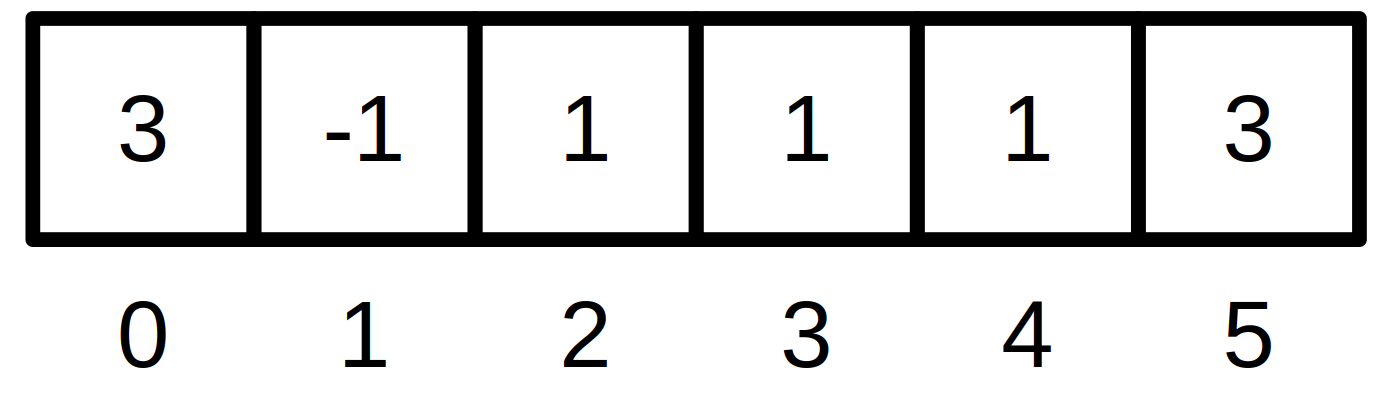
\includegraphics[width=0.9\linewidth]{lecon/10-arbres/arbre-tableau.png}
	\end{minipage}
\end{example}

\begin{rem}
	On ne stocke ici que la structure. Pour stocker des données, on produit un tableau de couples.
\end{rem}

\subsection{Représentation d'un arbre binaire presque complet}

\begin{definition}[Arbre binaire presque complet] \enspace\\
	\begin{minipage}{0.6\linewidth}
		Un arbre binaire presque complet est un arbre binaire dont tous les étages sont remplies sauf éventuellement le dernier qui est alors rempli à gauche
	\end{minipage} \qquad \begin{minipage}{0.4\linewidth}
		\begin{tikzpicture}[-]
			\node[state, scale=0.3] (q0) {};
			\node[state, scale=0.3, below left = 0.25 cm and 0.8cm of q0] (q1) {};
			\node[state, scale=0.3, below right = 0.25 cm and 0.8cm of q0] (q2) {};
			\node[state, scale=0.3, below left = 0.25 cm and 0.4cm of q1] (q3) {};
			\node[state, scale=0.3, below right = 0.25 cm and 0.4cm of q1] (q4) {};
			\node[state, scale=0.3, below left = 0.25 cm and 0.4cm of q2] (q5) {};
			\node[state, scale=0.3, below right = 0.25 cm and 0.4cm of q2] (q6) {};
			\node[state, scale=0.3, below left = 0.25 cm and 0.1cm of q3] (q7) {};
			\node[state, scale=0.3, below right = 0.25 cm and 0.1cm of q3] (q8) {};
			\node[state, scale=0.3, below left = 0.25 cm and 0.1cm of q4] (q9) {};
			
			\draw (q0) edge[] (q1);
			\draw (q0) edge[] (q2);
			\draw (q1) edge[] (q3);
			\draw (q1) edge[] (q4);
			\draw (q2) edge[] (q5);
			\draw (q2) edge[] (q6);
			\draw (q3) edge[] (q7);
			\draw (q3) edge[] (q8);
			\draw (q4) edge[] (q9);
		\end{tikzpicture}
	\end{minipage}
\end{definition}

\begin{minipage}{0.45\linewidth}
	\begin{principe}
		On peut alors représenter un tas par un tableau. On numérote alors les sommets ci contre, donnant l'indice dans le tableau. Les fils du noeuds d'indice $i$ se retrouve aux cases $2\times i+1$, $2\times i+2$, et son père $\left\lfloor \dfrac{i-1}{2}\right\rfloor$
	\end{principe}
\end{minipage}
\qquad
\begin{minipage}{0.45\linewidth}
	\begin{tikzpicture}[-]
		\node[state, scale=0.4] (q0) {};
		\node[state, scale=0.4, below left = 0.55 cm and 1.1cm of q0] (q1) {};
		\node[state, scale=0.4, below right = 0.55 cm and 1.1cm of q0] (q2) {};
		\node[state, scale=0.4, below left = 0.55 cm and 0.6cm of q1] (q3) {};
		\node[state, scale=0.4, below right = 0.55 cm and 0.6cm of q1] (q4) {};
		\node[state, scale=0.4, below left = 0.55 cm and 0.6cm of q2] (q5) {};
		\node[state, scale=0.4, below right = 0.55 cm and 0.6cm of q2] (q6) {};
		\node[state, scale=0.4, below left = 0.55 cm and 0.2cm of q3] (q7) {};
		\node[state, scale=0.4, below right = 0.55 cm and 0.2cm of q3] (q8) {};
		\node[state, scale=0.4, below left = 0.55 cm and 0.2cm of q4] (q9) {};
		
		\node[above right = 0cm and 0cm of q0] (l0) {\textcolor{cyan}{0}};
		\node[above left = 0cm and 0cm of q1] (l1) {\textcolor{cyan}{1}};
		\node[above right = 0cm and 0cm of q2] (l2) {\textcolor{cyan}{2}};
		\node[above left = 0cm and 0cm of q3] (l3) {\textcolor{cyan}{3}};
		\node[above right = 0cm and 0cm of q4] (l4) {\textcolor{cyan}{4}};
		\node[below = 0cm of q5] (l5) {\textcolor{cyan}{5}};
		\node[above right = 0cm and 0cm of q6] (l6) {\textcolor{cyan}{6}};
		\node[below = 0cm of q7] (l7) {\textcolor{cyan}{7}};
		\node[below = 0cm of q8] (l8) {\textcolor{cyan}{8}};
		\node[below = 0cm of q9] (l9) {\textcolor{cyan}{9}};
		
		\draw (q0) edge[] (q1);
		\draw (q0) edge[] (q2);
		\draw (q1) edge[] (q3);
		\draw (q1) edge[] (q4);
		\draw (q2) edge[] (q5);
		\draw (q2) edge[] (q6);
		\draw (q3) edge[] (q7);
		\draw (q3) edge[] (q8);
		\draw (q4) edge[] (q9);
	\end{tikzpicture}
\end{minipage}\\

\begin{example}\enspace\\
	\begin{minipage}{0.5\linewidth}
		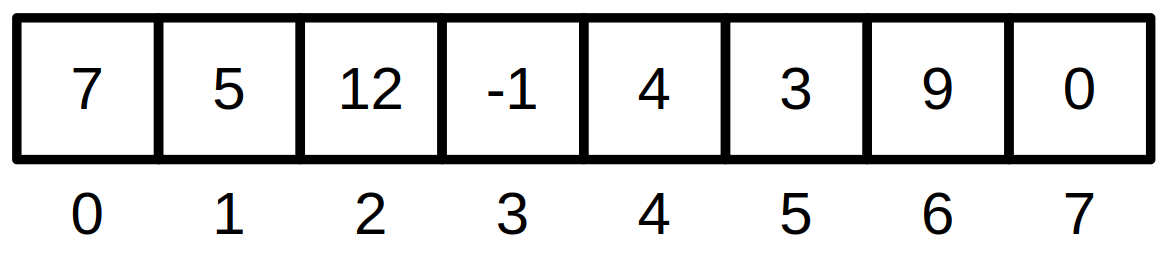
\includegraphics[width=\linewidth]{lecon/10-arbres/semi-complet.png}
	\end{minipage} \qquad
	\begin{minipage}{0.5\linewidth}
		\begin{tikzpicture}[-]
			\node[state] (q0) {7};
			\node[state, below left = 0.55 cm and 1.1cm of q0] (q1) {5};
			\node[state, below right = 0.55 cm and 1.1cm of q0] (q2) {12};
			\node[state, below left = 0.55 cm and 0.4cm of q1] (q3) {-1};
			\node[state, below right = 0.55 cm and 0.4cm of q1] (q4) {4};
			\node[state, below left = 0.55 cm and 0.4cm of q2] (q5) {3};
			\node[state, below right = 0.55 cm and 0.4cm of q2] (q6) {9};
			\node[state, below left = 0.55 cm and 0.2cm of q3] (q7) {0};
			
			\node[above right = 0cm and 0cm of q0] (l0) {\textcolor{cyan}{0}};
			\node[above left = 0cm and 0cm of q1] (l1) {\textcolor{cyan}{1}};
			\node[above right = 0cm and 0cm of q2] (l2) {\textcolor{cyan}{2}};
			\node[above left = 0cm and 0cm of q3] (l3) {\textcolor{cyan}{3}};
			\node[above right = 0cm and 0cm of q4] (l4) {\textcolor{cyan}{4}};
			\node[below = 0cm of q5] (l5) {\textcolor{cyan}{5}};
			\node[above right = 0cm and 0cm of q6] (l6) {\textcolor{cyan}{6}};
			\node[below = 0cm of q7] (l7) {\textcolor{cyan}{7}};
			
			\draw (q0) edge[] (q1);
			\draw (q0) edge[] (q2);
			\draw (q1) edge[] (q3);
			\draw (q1) edge[] (q4);
			\draw (q2) edge[] (q5);
			\draw (q2) edge[] (q6);
		\draw (q3) edge[] (q7);
		\end{tikzpicture}
	\end{minipage}
\end{example}

\section{Application}

\begin{com}
	A chaque fois on va écrire en début quelle représentation on utilise pour notre application. Néanmoins, en classe, on pourrait le laisser proposer par les élèves (une fois l'application présentée). On justifie de ce fait notre organisation, ou les applications arrivent toutes ensembles à la fin. (mais on écrit quand même la représentation au début pour que ce soit plus facile de naviguer à la partie que l'on souhaite).
\end{com}

\subsection{Dictionnaires}

\noindent \textbf{Représentation :} Structure inductive

\begin{definition}
	Un arbre binaire de recherche $N(x, G, D)$ est un arbre binaire de recherche (ABR) si $G$ et $D$ sont des ABR et si, selon un attribut $a$, $\max\limits_{u\in G} u.a\leq x.a \leq \min\limits_{v\in D} v.a$ (avec $E$ qui est un ABR et $\max\limits_{u\in E} u.a = -\infty$ et $\min\limits_{u \in E} u.a = +\infty$)
\end{definition}

\begin{proposition}
	Chercher et insérer dans un ABR est en $O(h)$
\end{proposition}

\begin{proposition}
	En imposant des contraintes supplémentaires (exemple arbres rouge-noir), on peut forcer $h = O(\log n)$
\end{proposition}

\begin{definition}
	Un dictionnaire (ou tableau associatif) est un tableau où les indices (clés) ne se limite pas à $\llbracket 0, n\rrbracket$
\end{definition}

\begin{idee}
	On peut alors implémenter un dictionnaire par un ABR, les clés étant les étiquettes des nœuds, à condition d'avoir un ordre total sur les clés
\end{idee}

\begin{theorem}
	Une implémentation efficace des dictionnaires par ABR permet des opérations de base en $O(\log n)$
\end{theorem}

\begin{com}
	Si on ne veut pas faire le développement 2, et qu'on préfère celui sur les arbres k-dimensionnel, on peut aussi parler aussi du pb des k-plus proches voisins et parler des ABR comme des arbres k-dim pour résoudre le pb
\end{com}

\subsection{Classes d'équivalence}

\noindent \textbf{Représentation :} Tableaux

\begin{definition}
	Une structure union \& trouver est une structure implémentant les classes d'équivalence, permettant de trouver les représentants d'une classe et d'unir deux classes.
\end{definition}

\begin{idee}
	On implémente cette structure sous formes d'un ensemble d'arbres (forêt), où chaque arbre représente une classe et où la racine est le représentant de la classe
\end{idee}

\begin{example}
	La relation d'égalité modulo 3 sur $\llbracket 0, 7 \rrbracket$ peut être représenté par : \\
	\begin{minipage}{0.4\linewidth}
		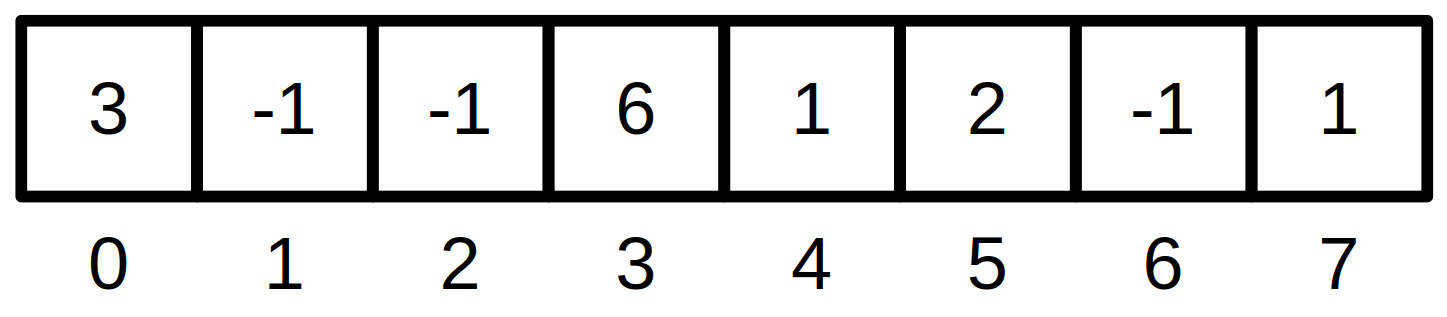
\includegraphics[width=\linewidth]{lecon/10-arbres/classe_equiv.png}
	\end{minipage}
	\qquad
 	\begin{minipage}{0.4\linewidth}
 		\begin{tikzpicture}[->, node distance=2cm]
 			\node[state] (q0) {$1$};
 			\node[state, below left of = q0] (q1) {$4$};
 			\node[state, below right of = q0] (q2) {$7$};	
 			\node[state, right = 2.5cm of q0] (q3) {$2$};
 			\node[state, below of = q3] (q4) {$5$};
 			\node[state, above right = 0.2cm and 2cm of q3] (q5) {$6$};
 			\node[state, below of = q5] (q6) {$3$};
 			\node[state, below of = q6] (q7) {$0$};
 			
 			\draw (q0) edge[] (q1);
 			\draw (q0) edge[] (q2);
 			\draw (q3) edge[] (q4);
 			\draw (q5) edge[] (q6);
 			\draw (q6) edge[] (q7);
 		\end{tikzpicture}
 	\end{minipage}
\end{example}

\begin{proposition}
	Si on unifie en faisant pointer la racine de l'arbre le moins profond vers celle de l'arbre le plus profond, on obtient des opérations unir et trouver en $O(\log(n))$
\end{proposition}

\subsection{Arbres couvrant de poids minimal}

\noindent \textbf{Représentation :} liste des arêtes

\begin{definition}
	Dans un graphe pondéré connexe, un arbre couvrant de poids minimal, est un sous-ensemble maximal d'arêtes sans cycles de somme de poids minimal.
\end{definition}

\begin{algorithm}[H]
	\caption{$Kruskal(L)$}
	\Entree{$L$ liste des arêtes}
	\Sortie{Liste des arêtes d'un ACM}
	$L\gets L$ trié\\
	$res \gets []$\\
	\Pour{$a$ parcourant $L$}
	{
		\Si{$a$ ne rajoute pas de cycle dans $res$}
		{
			Ajouter $a$ à $res$
		}
	}
	\Retour{$res$}
\end{algorithm}

\begin{proposition}
	En implémentant la détection de cycle par une structure union \& trouver, Kruskal renvoie un arbre couvrant de poids minimal en $O(|L| \times \log |L|)$
\end{proposition}

\subsection{Files de priorité}

\noindent \textbf{Représentation :} celles des arbres semi-complet

\begin{definition}
	Une file de priorité est une séquence de données dont on peut extraire la donnée d'attribut minimum, et rajouter des données.
\end{definition}

\begin{idee}
	On peut implémenter les files de priorité par des tas min
\end{idee}

\begin{definition}
	Un tas min est un arbre semi-complet où chaque noeud a un attribut plus petit que ses fils
\end{definition}

\noindent \textbf{Développement 2 :} Correction de l'insertion dans un tas min et discussion sur l'implémentation

\begin{principe}
	\enspace
	\begin{itemize}[label=$\star$]
		\item Pour ajouter un élément, on le met au bout du tablea et on l'échange avec son père tant qu'il est plus petit
		\item, Pour extraire le min, on met le dernier élément du tableau au début et on l'inverse avec le plus petit de ses fils tant qu'il est plus grand.
	\end{itemize}
\end{principe}

\begin{proposition}
	Cette implémentation permet des opérations en $O(\log n)$
\end{proposition}

\begin{appl}
	Trier par tas en $O(n \log n)$
\end{appl}

\chapter{Exemples d'algorithmes d'approximation et d'algorithmes probabilistes}
\label{L11}
\dev{Emile Martinez}{}

Beaucoup de problèmes sont durs à résoudre. On cherchera alors à sacrifier un peu de la fiabilité du résultat pour gagner en complexité. Il y a deux manières de faire un tel compromis : \begin{itemize}
	\item utiliser des algorithmes probabilistes (pouvant prendre beaucoup de temps, ou renvoyer faux)
	\item n'utiliser des algorithmes ne fournissant que des solutions approchées.
\end{itemize}

\section{Algorithmes probabilistes}

\begin{definition}
	Un algorithme est déterministe si, pour une entrée x donnée, il s’exécute toujours de la même manière. En particulier, la sortie ne dépend que de l'entrée.
	
	Un algorithme probabiliste est un algorithme dont l'exécution dépend de son entrée x et de valeurs obtenues via un générateur de nombre (pseudo)-aléatoire.
\end{definition}

\begin{example}
	\label{11-prem-ex}
	\normalfont
	Recherche dans un tableau $T$ de booléens d'un indice $i$ tel que $T[i] == True$\\
	\begin{minipage}{0.45\linewidth}
		\begin{algorithm}[H]
			\caption{$deterministe(T)$}
			\Pour{$i$ de $1$ à $|T|$}{
				\Si{$T[i]$}
				{
					\Retour{True}
				}
			}
			\Retour{False}
		\end{algorithm}
	\end{minipage} \qquad
	\begin{minipage}{0.45\linewidth}
		\begin{algorithm}[H]
			\caption{$probabiliste(T, k)$}
			\Pour{$j$ de $1$ à $k$}{
				Tirer uniformément $i$ dans $\llbracket 1, n \rrbracket$\\
				\Si{$T[i]$}
				{
					\Retour{True}
				}
			}
			\Retour{False}
		\end{algorithm}
	\end{minipage}
\end{example}

\begin{rem}
	Soit $p<1$ la proportion de booléen à Faux dans $T$. Alors l'algo probabiliste se trompe avec une probabilité = $p^k$.	
	Pour $p = \frac{1}{4}$ et $k=5$, cela fait $10^{-3}$
\end{rem}

\subsection{Algorithme de type Monte-Carlo}

\begin{definition}
	Un algorithme probabiliste A pour un pb P est de type Monte-Carlo si pour toute instance i de P, \begin{itemize}
		\item $A(i)$ est une solution, erronée avec une certaine probabilité
		\item Le temps d'exécution de $A$ sur $i$ est indépendant des choix aléatoires.
	\end{itemize} 
\end{definition}

\begin{example}
	L'algorithme probabiliste de l'exemple \ref{11-prem-ex} est de type Monte-Carlo
\end{example}

\textbf{Développement 1 :} Vérification probabiliste du produit matriciel

\begin{proposition}[Amplification]
    Soient $0 < \varepsilon_2 < \varepsilon_1 < 1$.
    
	S’il existe un algorithme Monte Carlo pour un problème $\Pi$ ayant une probabilité d’erreur $\varepsilon_1$, alors on peut construire un algorithme Monte Carlo pour le problème $\Pi$ ayant une probabilité d’erreur $\varepsilon_2$, en appliquant plusieurs fois l'algorithme initial.
\end{proposition}

\begin{algorithm}[H]
	\label{11-mediane}
	\caption{$mediane(L)$}
	$n \gets |L|$\\
	$L_{0} \gets k = n^{\frac{3}{4}}$ éléments de $L$ aléatoirement\\
	Trier $L_0$\\
	$x_1 \gets L_0[\frac{k}{2} - \sqrt{n}]$\\
	$x_2 \gets L_0[\frac{k}{2} + \sqrt{n}]$\\
%	$L_1, \, L_2, \, L_3 \gets[], \, [], \, []$\\
%	\Pour{$x \in L$}
%	{
%		\eSi{$x \leq x_1$}
%		{
%			Ajouter $x_1$ à $L_1$
%		}{
%		\eSi{$x \leq x_2$}
%		{
%			Ajouter $x$ à $L_2$
%		}
%		{
%			Ajouter $x$ à $L_3$
%		}
%		}
%	}
	$L_1 \gets $ liste des éléments $< x_1$\\
	$L_2 \gets$ liste des éléments entre $x_1$ et $x_2$\\
	$L_3 \gets$ liste des éléments $> x_2$\\
	\Si{$|L_1| > \frac{n}{2}$ ou $|L_3| > \frac{n}{2}$}{\Retour{n'importe quoi}\tcp*{$L_2$ n'a pas capturé la médiane}}
	\Si{$|L_2| > n^{\frac{3}{4}}$}{\Retour{n'importe quoi}\tcp*{On a trop d'éléments dans $L_2$ pour les trier}}
	Trier $L_2$\\
	\Retour{$L_2[\frac{n}{2} - |L_1|]$}
\end{algorithm}

\begin{idee}
	On fait la médiane sur un échantillon de $L$. Puis on prend tous les éléments autour de cette médiane et on les trie pour trouver la vraie médiane (si elle y est, sinon tant pis).
\end{idee}

\begin{com}
	Ici le temps dépend du hasard. On considère quand même que c'est un Monte Carlo car c'est borné et prend le temps moyen est un $\Omega$ du temps dans le pire des cas. On pourrait aussi a la place de retourner n'importe quoi, trier $n^{3/4}$ éléments et remplir $L_2$ avec des $= \infty$ mais alors on complexifie pour rien.
\end{com}

\subsection{Algorithmes de type Las Vegas}

\begin{definition} 
	Un algorithme probabiliste $A$ est de Las Vegas si :
	\begin{itemize}
		\item Si $A$ termine, alors la solution renvoyée est correcte.
		\item Le temps d'exécution de $A$ est une variable aléatoire.
	\end{itemize}
\end{definition}

\begin{rem}
	Quand on parle de complexité en moyenne pour un algorithme de Las Vegas, on ne considère pas (ou pas uniquement) la moyenne des complexité sur toutes les entrées possibles prisent uniformément, mais la plus grande espérance du temps d'exécution sur une entrée
\end{rem}


\begin{algo}
	\normalfont \enspace\\
	\label{11-tri-rapide}
	\begin{algorithm}[H]
		\caption{$tri\_rapide\_randomise(T)$}
		\Si{$|T| = 1$}{\Retour}
		Tirer $q$ uniformément dans $\llbracket 1, |T| \rrbracket$ \tcp*{$T[q]$ sera le pivot}
		$i \gets partition(T, q)$\\
		$tri\_rapide\_randomise(T[:i])$\\
		$tri\_rapide\_randomise(T[i+1:])$\\
	\end{algorithm}
	où $partition(T, q)$ mets dans $T$, tous les éléments $< T[q]$ puis tous les éléments supérieurs, et renvoie l'indice du milieu.
\end{algo}

\begin{rem}
	Le temps d'exécution de l'algorithme \ref{11-tri-rapide} dépend du choix du pivot : $O(n^2)$ dans le pire cas, $O(n\log n)$ dans le meilleur et en moyenne. 
\end{rem}

\begin{rem}
	Il est possible de transformer un algorithme de type Las Vegas en Monte Carlo en l'exécutant pendant un temps défini et en générant une réponse aléatoire s'il n'a pas terminé.
\end{rem}

\begin{rem}
	Si on peut vérifier efficacement la validité du résultat, on peut également faire l'inverse.
\end{rem}

\begin{example}
	A la place de l'échec dans l'algorithme \ref{11-mediane}, on peut relancer l'algorithme. On obtient alors un algorithme trouvant toujours la médiane, la calculant en moyenne en $1,5n$ comparaisons, sans adversaires, ce qui est mieux que tout algorithme déterministe (qui ont nécessairement besoin d'au moins $2n$ comparaisons en moyenne).
\end{example}

\section{Algorithmes d'approximation}

\subsection{Définition}


\begin{definition}
	Un problème d’optimisation est un problème $\Pi = (I, S, c)$ où \begin{itemize}
		\item $I$ est l'ensemble des instances
		\item $\forall i \in I, S(i)$ est l'ensemble des solutions pour $i$
		\item $c : I \times S \to R$ fonction d'évaluation.
	\end{itemize}
	Étant donnée une instance $i \in I$, l’objectif est de construire une solution $s^{*} \in S(i)$ vérifiant : $c(i, s^{*}) = \min\left\{c(x, s) \big/ s \in S(i)\right\}$
\end{definition}

\begin{com}
	On peut aussi demander à ce que $c$ soit calculable en temps polynomial mais ce n'est pas nécessaire. Les deux définitions coexistent.
\end{com}

\begin{rem}
	On se ramène au max en prenant $-c$.
\end{rem}

\begin{definition}
	    Une $\lambda$-approximation est un algorithme polynomial $A$ donnant pour chaque instance $i$ de $\Pi$ une solution tel que $\max\left(\left| \dfrac{A(i)}{OPT(i)} \right|, \left| \dfrac{OPT(i)}{A(i)} \right|\right) \leq \lambda$
\end{definition}

\subsection{Exemples}

\begin{definition}[Couvertue par des sommets (Vertex-Cover)]
	Entrée : Un graphe $G = (S, A)$
	Solution : Un ensemble $S \subset V$ tel que $\forall u, v \in E, \,v\in S \text{ ou } u \in S$
\end{definition}

\begin{algorithm}[H]
	\label{11-glouton-vc}
	\caption{Glouton Vertex Cover}
	$S \gets \{\}$\\
	\Tq{il existe une arête $(u,v) \in A$ tel que $u\notin S$ et $v \notin S$}
	{
		Choisir $(u,v)$ une telle arête\\
		$S \gets S \cup \{(u,v)\}$
	}
	\Retour{$S$}
\end{algorithm}

\begin{proposition}
	L'algorithme \ref{11-glouton-vc} est une 2-approx du problème de la couverture par les sommets.
\end{proposition}



\noindent \textbf{Développement :} Une $\frac{3}{2}$-approximation et une $\frac{7}{6}$-approximation gloutonnes pour le problème d'ordonnancement de tâches indépendantes sur 2 processeurs.



\begin{definition}[Voyageur de commerce (TSP)]
	Instance : $G = (S, A, c)$ un graphe orienté complet pondéré\\
	Solution : Un cycle hamiltonien sur $G$ de poids minimal
\end{definition}

\begin{theorem}
	Il n'existe pas d'algorithme d'approximation pour TSP, sauf si $P = NP$.
\end{theorem}

\begin{algo}[Algorithme pour TSP]
	\label{11-approx-tsp}
	\enspace \begin{enumerate}
		\item $\mathcal A \gets$ arbre couvrant de poids minimal de $G$
		\item $P \gets$ parcours en profondeur préfixe de $\mathcal A$
		\item Renvoyer $P$
	\end{enumerate}
\end{algo}

\begin{proposition}
	L'algorithme \ref{11-approx-tsp} est une 2-approx si $c$ vérifie l'inégalité triangulaire ($\forall x, y, z\in C, \, c(x, y) + c(y, z) \geq c(x, z)$)
\end{proposition}

\begin{example} \normalfont \enspace \\
	\begin{tikzpicture}[-]
		%etape 1
		\node[state, scale=0.4] (a0) {};
		\node[state, scale=0.4, below left = 1cm and 0.75cm of a0] (a1) {};
		\node[state, scale=0.4, below right = 1cm and 0.75cm of a0] (a2) {};
		\node[state, scale=0.4, above right = 0.4cm and 1.2cm of a0] (a3) {};
		\node[state, scale=0.4, above = 1.2cm of a0] (a4) {};
		\node[state, scale=0.4, above left = 0.4cm and 1.2cm of a0] (a5) {};
		
		\draw (a0) edge[green] (a1);
		\draw (a0) edge[green] (a2);
		\draw (a0) edge[green] (a3);
		\draw (a0) edge[green] (a4);
		\draw (a0) edge[green] (a5);
		
		\draw (a1) edge[black] (a2);
		\draw (a2) edge[black] (a3);
		\draw (a3) edge[black] (a4);
		\draw (a4) edge[black] (a5);
		\draw (a5) edge[black] (a1);
		
		\draw (a1) edge[red] (a3);
		\draw (a2) edge[red] (a4);
		\draw (a3) edge[red] (a5);
		\draw (a4) edge[red] (a1);
		\draw (a5) edge[red] (a2);
		
		%légende
		\node[below left = 1cm and 0cm of a1] (l1) {};
		\node[right = 0.5cm of l1] (l2) {};
		\node[right = 0cm of l2] {coût 1};
		\node[below = 0.2cm of l1] (l3) {};
		\node[right = 0.5cm of l3] (l4) {};
		\node[right = 0cm of l4] {coût 1};
		\node[below = 0.2cm of l3] (l5) {};
		\node[right = 0.5cm of l5] (l6) {};
		\node[right = 0cm of l6] {coût 2};
		
		\draw (l1) edge[red] (l2);
		\draw (l3) edge[green] (l4);
		\draw (l5) edge[black] (l6);
		
		%flèche 1
		\node[below right = 0.9cm and 1.4cm of a0] (f1) {};
		\node[below right = 0.6cm and 0.9cm of f1] (f2) {};
		
		\draw (f1) edge[->, above right] node{1} (f2);
		
		%etape 2
		\node[state, scale=0.4, label = {[yshift=-1cm]A}, below right = 1.1cm and 1.6 cm of f2] (b0) {};
		\node[state, scale=0.4, label = B, below left = 1cm and 0.75cm of b0] (b1) {};
		\node[state, scale=0.4, label = C, below right = 1cm and 0.75cm of b0] (b2) {};
		\node[state, scale=0.4, label = D, above right = 0.4cm and 1.2cm of b0] (b3) {};
		\node[state, scale=0.4, label = E, above = 1.2cm of b0] (b4) {};
		\node[state, scale=0.4, label = F, above left = 0.4cm and 1.2cm of b0] (b5) {};
		
		\draw (b0) edge[green] (b1);
		\draw (b0) edge[green] (b2);
		\draw (b0) edge[green] (b3);
		\draw (b0) edge[green] (b4);
		\draw (b0) edge[green] (b5);
		
		%flèche 2
		\node[above = 0.7cm of b4] (f3) {};
		\node[above = 0.9cm of f3] (f4) {};
		
		\draw (f3) edge[->, right] node{2} (f4);
		
		%etape 3
		\node[above = 0cm of f4] (c0) {ABCDEFA};
		
		%flèche 3
		\node[below right = 0cm and 0.5cm of c0] (f5) {};
		\node[below right = 0.6cm and 2cm of f5] (f6) {};
		
		\draw (f5) edge[->, above right] node{3} (f6);
		
		%etape 4
		\node[state, scale=0.4, below right = 1cm and 1.8cm of f6] (d0) {};
		\node[state, scale=0.4, below left = 1cm and 0.75cm of d0] (d1) {};
		\node[state, scale=0.4, below right = 1cm and 0.75cm of d0] (d2) {};
		\node[state, scale=0.4, above right = 0.4cm and 1.2cm of d0] (d3) {};
		\node[state, scale=0.4, above = 1.2cm of d0] (d4) {};
		\node[state, scale=0.4, above left = 0.4cm and 1.2cm of d0] (d5) {};
		
		\draw (d0) edge[green] (d1);
		\draw (d1) edge[black] (d2);
		\draw (d2) edge[black] (d3);
		\draw (d3) edge[black] (d4);
		\draw (d4) edge[black] (d5);
		\draw (d5) edge[green] (d0);
		
		%conclusion
		\node[below = 1.5cm of d0] {On a un coût de 10 et non de 6};
		
	\end{tikzpicture}
\end{example}

\section{Algorithmes d'approximation probabilistes}

Il existe des algorithmes d'approximation probabilistes. Ce sont alors souvent des algorithmes de Monte Carlo.

\subsection{Max Sat}

\begin{definition}
	Instance : $n$ variables $\{x_1, \dots, x_n\}$, p clauses $C_1, \dots, C_p$ sur $(x_1, \dots, x_n$) contenant au moins k littéraux
	Solution : Trouver une valuation maximisant le nombre de clauses à vrai
\end{definition}

\begin{example}
	Si $\varphi = \bigwedge\limits_{i=1}^p C_i$ est satisfiable, une solution optimale est une valuation satisfaisant $\varphi$
\end{example}

\begin{algo}
	Renvoyer une valuation aléatoire.
\end{algo}

\begin{theorem}
	L'espérance du nombre de clauses satisfaites $\mathbb E(\varphi)$ vérifie $\mathbb E(\varphi) \geq p\left( 1 - \dfrac{1}{2^k}\right) \geq \dfrac{c}{2}$
\end{theorem}

\begin{rem}
	On peut créer un algorithme déterministe qui est une $\left( 1 - \dfrac{1}{2^k} \right)$-approx.
\end{rem}

\subsection{Calcul de $\pi$}

On peut calculer une valeur approchée de $\pi$ par des méthodes probabilistes

\begin{algorithm}
	\caption{$calcul\_pi(N)$}
	$i \gets O$\\
	\Repeter{$N$ fois}
	{
		Tirer deux flottants $x, y$ dans $[-1, 1]$ uniformément\\
		\Si{$x^2+y^2 < 1$ }
		{
			$i \gets i+1$ \tcp*{On a tapé dans le cercle d'aire $\pi$}
		}
	}
	\Retour $\dfrac{4i}{N}$\tcp*{Nombre de points dans le cercle / aire du carré = $\frac{\pi}{4}$}
\end{algorithm}

\begin{com}
	On peut aussi mettre un dessin ici pour expliquer ce qui se passe.
\end{com}

\begin{com}
	Si on veut parler plus précisément d'algorithme d'approximation, on prendrait dans la def, pour $I$ la manière de représenter les flottants (nb de bits d'exposant, de mentisse, etc\dots) et pour $S$ de tels flottants. La fonction de coût $c$ serait alors la distance à $pi$ (même si pas facilement calculable en temps polynomial)
\end{com}

\begin{rem}
	On peut généraliser la méthode pour le calcul d'intégrales
\end{rem}

\begin{rem}
	Cette méthode se généralise en une méthode de Monte Carlo où l'on échantillone le problème, on calcule la solution sur cette échantillon, puis on généralise la solution à partir de cet échantillon.
\end{rem}

\chapter{Exemples d'algorithmes glouton et de retour sur trace}
\label{L12}
\dev{Emile Martinez}{}

Quand on aborde un problème à la main, on essaye souvent de construire des solutions au fur et à mesure, en faisant plein de choix locaux. Essayons de mettre cela en oeuvre algorithmiquement.

\section{Algorithmes gloutons}

\subsection{Définition}

\begin{definition}
	Un algorithme glouton construit une solution à un problème par choix successifs considérés localement optimaux, sans jamais revenir en arrière.
\end{definition}

\textbf{Avantage :} C'est souvent peu coûteux, et potentiellement en ligne.

\begin{example}[Gymnases]\enspace
	\begin{itemize}
		\item[Instances :] $n$ évènements, leur date de début $\left\{d_i\right\}_{i \in \{1, \dots, n\}}$ et de fin $\left\{f_i\right\}_{i \in \{1, \dots, n\}}$
		\item[Problème :] trouver un nombre minimal de gymnases pour organiser les évènements
	\end{itemize}
\end{example}

\begin{algo}\enspace
	\begin{enumerate}
		\item Trier les évènements par dates de début croissantes
		\item Allouer successivement le premier gymnase disponible. En ouvrir un si nécessaire.
	\end{enumerate}
\end{algo}

\chapter{Exemples d’algorithmes utilisant la méthode « diviser pour régner »}
\label{L13}
\dev{Emile Martinez}{}

\section{Introduction}

\begin{definition}[Paradigme Diviser pour Régner]Un algorithme de type Diviser pour Régner s'effectue en 3 étapes : \begin{enumerate}
		\item Division du problème en sous-problèmes indépendants
		\item Résolution récursive des sous-problèmes
		\item Construction d'une solution du problème global à partir des solutions des sous-problèmes
\end{enumerate}
	
\end{definition}

\begin{principe}[Calcul de la compléxité d'un tel algorithme.]
	
	Trouver une fonction donnant la taille du problème (comme le nombre d'éléments pour une liste). Définir $C$ la complexité maximale des instances de cette taille, puis trouver une relation de réccurence sur $C$, pour tenter de la résoudre.
	
\end{principe}

\begin{com}
	La méthode de résolution sera inculqué par l'exemple, et progressivement (d'abord le cas de base, où l'on découpe en seulement 2 avec l'exponentiation rapide, puis on complexifie)
\end{com}

\section{Applications au calcul formel}

\subsection{L'exponentiation rapide}

\textbf{Problème :} Étant donné un entier $a$ et un entier positif $n$, calculer $a^n$.

\textbf{Solution naïve :} $n$ multiplications

\begin{algo}[Méthode D\&R] \enspace \\
	\begin{minipage}{0.7\linewidth}
		\begin{algorithm}[H]
			\caption{$exponentiation\_rapide(a, n)$}
			\Si{$n = 0$}
				{\Retour{$1$}}
			$m \gets m/2$ \tcp*{étape 1}
			$x \gets exponentiation\_rapide(a, m)$ \tcp*{étape 2}
			\eSi(\tcp*{étape 3}){$n$ est pair}
				{\Retour{$x\times x$}}
				{\Retour{$x\times x \times a$}}
		\end{algorithm}
	\end{minipage}
\end{algo}

\begin{proposition}[Complexité]
	La complexité en nombre de multiplication par rapport à l'entier positif (noté $C(n)$) vaut $C(n) = O\big(\log(n)\big)$
\end{proposition}

\begin{proof}
	\label{13-preuve}
	\begin{enumerate}
		\item $C(n) = C\left(\left\lfloor\dfrac{n}{2}\right\rfloor \right) + O(1)$
		\item $C$ est majoré par $D(n) = D\left(\left\lfloor\dfrac{n}{2}\right\rfloor\right) + K$
		\item $D$ est croissante
		\item $D\left(2^k\right)$ est une suite arithmétique donc $D\left(2^k\right) = O(k)$
		\item $C(n) \underset{\substack{\uparrow\\2}}\leq D(n) \underset{\substack{\uparrow\\3}}\leq D\left(2^{\left\lfloor\log(n)\right\rfloor+1}\right) \underset{\substack{\uparrow\\4}}= O(\log(n))$
	\end{enumerate}
\end{proof}

\subsection{Multiplication matricielle}

\textbf{Problème :} Étant donné $A = (a_{i,j})$ et B = $(b_{i,j})$ deux matrices de taille $n$, on cherche à calculer $A_\times B$

\textbf{Solution naïve :} $O(n^3)$
\begin{algo}[Méthode D\&R : Algorithme de Strassen]
	\begin{enumerate}
		\item Rajouter des 0 pour que $A$ et $B$ soient de tailles paires. Diviser alors $A$ et $B$ en matrices de taille $\frac{n}{2}$
		$$A = \left( \begin{array}{c|c}
			A_{1, 1} & A_{1, 2} \\ \hline
			A_{2, 1} & A_{2, 2}
		\end{array}\right) \text{ et } B = \left( \begin{array}{c|c}
		B_{1, 1} & B_{1, 2} \\ \hline
		B_{2, 1} & B_{2, 2}
		\end{array}\right)$$
		
		\item Calculer récursivement \\
		$M_1 = (A_{1, 1} + A_{2, 2}) \times (B_{1, 1} + B_{2, 2}) $\\
		$M_2 = (A_{2, 1} + A_{2,2}) \times B_{1, 1} $\\
		$M_3 = A_{1, 1} \times (B_{1, 2} - B_{2, 1})$\\
		$M_4 = A_{2, 2} \times (B_{2, 1} - B_{1, 1})$\\
		$M_5 = (A_{1, 1} + A_{1, 2}) \times B_{2, 2}$\\
		$M_6 = (A_{2, 1} - A_{1, 1}) \times (B_{1, 1} + B_{1, 2})$\\
		$M_7 = (A_{1, 2} - A_{2, 2}) \times (B_{2, 1} + B_{2, 2})$\\
		
		\item Calculer $A\times B = \left( \begin{array}{c|c}
			M_1 + M_4 - M_5 + M_7 & M_3 + M_5 \\ \hline
			M_2 + M_4 & M_1 - M_2 + M_3 + M_6
		\end{array}\right)$
		
	\end{enumerate}
\end{algo}

\begin{exercise}
	Prouver la correction de l'algorithme de Strassen.
\end{exercise}

\begin{proposition}
	Cette algorithme a une complexité en $O\left( n ^{\log_2(3)}\right)$
\end{proposition}

\begin{exercise}
	Prouver cela en reprenant la preuve pour l'exponentiation en considérant $\dfrac{D(2^k)}{7^k}$ à l'étape 4 de la preuve \ref{13-preuve}
\end{exercise}

\section{Application aux listes}
	
\subsection{Recherche dichotomique}

\label{13-dico}

\textbf{Problème :} Rechercher un élément $a$ dans une liste $L$ d'éléments triés selon un ordre $\leq$

\begin{algorithm}[H]
	\Entree{$L$ une liste triée, $a$ un élément}
	\Sortie{$i$ tel que $L[i] = a$ s'il existe, $-1$ sinon}
	\caption{$recherche\_dichotomique(l, a, debut, fin)$}
	\Si{$fin < debut$}
		{\Retour $-1$}
	$m \gets \left\lfloor \dfrac{debut + fin}{2}\right\rfloor$ \\
	\Si{$l[m] =- a$}
		{\Retour $m$}
	\eSi{$l[m] < a$}
		{\Retour{$recherche\_dichotomique(l, a, m+1, fin)$}}
		{\Retour{$recherche\_dichotomique(l, a, debut, m+1)$}}
\end{algorithm}

\begin{exercise}
	Ecrire le code en plus de lignes et faire apparaître les 3 étapes de D\&R
\end{exercise}

\begin{proposition}
	La recherche dichotomique est en $O(\log |L|)$
\end{proposition}

\begin{exercise}
	Écrire une version itérative de cet algorithme
\end{exercise}

\subsection{Tri fusion}
\label{13-tri-fusion}

\begin{algorithm}[H]
	\caption{$fusion(L_1, L_2)$}
	\Entree{$L_1$, $L_2$ deux listes triées d'éléments comparables}
	\Sortie{La fusion des listes $L_1$ et $L_2$ triée}
	$res \gets []$\\
	$i,j \gets 0$\\
	\Tq{
		$i < |L_1|$	et $j < |L_2|$
	}{
		\eSi{$L_1[i] < L_2[j]$}{
			$res$.ajouter($L_1[i]$) \\
			$i \gets i + 1$
		}{
			$res$.ajouter($L_2[j]$) \\
			$j \gets j + 1$
		}
	}
	Ajouter le reste de $L_1$ et de $L_2$ à $res$\\
	\Retour{$res$}
\end{algorithm}

\begin{algorithm}[H]
	\caption{$tri\_fusion(L)$}
	\Entree{Une liste $L$ d'éléments comparables}
	\Sortie{La liste $L$ triée}
	$n \gets |L|$\\
	\Si{$n\leq 1$}{
		\Retour{$L$}
	}
	$L_1, L_2 \gets partionner(L)$ \tcp*{Étape 1}
	$A \gets tri\_fusion(L_1)$ \tcp*{Étape 2}
	$B \gets tri\_fusion(L_2)$
	\Retour{$fusion(A, B)$}
\end{algorithm}

\begin{proposition}
	Le tri fusion est $O(n \log n)$ avec $n = |L|$
\end{proposition}

\begin{proof}
	Exercice
\end{proof}

\textbf{Développement :} Correction et terminaison du tri fusion

\begin{appl}
	Si l'on veut chercher si $K$ entiers sont présents parmi $N$, on peut avec \ref{13-dico} et \ref{13-tri-fusion} faire cela en $O\big((N + K) \log N \big)$ au lieu de $O(k\times N)$
\end{appl}



\subsection{Tri rapide}

\textbf{Objectif :} Faire un tri D\&R en place

\begin{com}
	Ici, on peut avoir des questions sur le tri fusion en place, ce qui existe plus ou moins mais est assez pénible. Donc ca peut valoir le coup de se renseigner sur le sujet.
\end{com}

\begin{idee}
	Choisir un élément appelé pivot et mettre à gauche tous les éléments plus petit, à droite tous les plus grands, puis à trier cette partie à droite et à gauche.
\end{idee}

\begin{algorithm}
	\caption{$tri\_rapide(L, debut, fin)$}
	\Si{$debut \geq fin -1$}
	{\Retour{$L$}}	
	$pivot \gets L[0]$\\	
	$i \gets debut$\\
	$j \gets fin$\\
	\Tq{$i < j$}
	{
		\eSi{$L[i+1] \leq pivot$}
		{
			échanger $L[i+1]$ et $L[i]$\\
			$i \gets i+1$
		}{		
			échanger $L[i+1]$ et $L[j]$\\
			$j \gets j - 1$
		}
		
		$tri\_rapide(L, debut, i-1)$\\	
		$tri\_rapide(L, i+1, fin)$\\
	}
\end{algorithm}

\begin{com}
	Par manque de place, on peut remplacer l'écriture de cet algorithme par un dessin expliquant l'idée, et mettre son écriture en exercice.
\end{com}

\begin{proposition}
	Ce tri est dans le pire des cas en $O(n^2)$, dans le cas moyen en $O(n \log n)$. Il est néanmoins en place (en autorisant un espace non pas constant mais logarithmique).
\end{proposition}

\begin{com}
	L'occasion de briller sur le fait que le tri rapide écrit comme ça n'est pas en place avec la définition première, mais l'est avec la définition élargie où on autorise $O(\log n)$ espace (utilisé par les appels récursifs)
\end{com}

\section{Application Géométrique}

\subsection{Plus petite distance dans le plan}

\textbf{Problème :} Étant donné $n$ points de $\mathbb R^2$, donner la plus petite distance entre deux points

\textbf{Solution naïve :} $n$ multiplications

\begin{algo}[Solution D\&R]
	\begin{enumerate}
		\item Choisir une abscisse $x_m$ séparant les points en deux sous-ensembles $P_1$ et $P_2$ de taille égale (à + ou - 1)
	
		\item Trouver les plus petites distances $d_1$ et $d_2$ de $P_1$ et $P_2$
	
		\item Rechercher la plus petite distance $d_3$ entre deux points dans la bande d’abscisse $[x_m-d_0, x_m+d_0]$ pour $d_0$ = $\min d_1, d_2$
	
	\end{enumerate}
\end{algo}

L'étape 3 peut se faire en ne regardant que les 7 points suivants (suivants au sens de l'ordonnée).\\
\begin{minipage}{0.35\linewidth}
	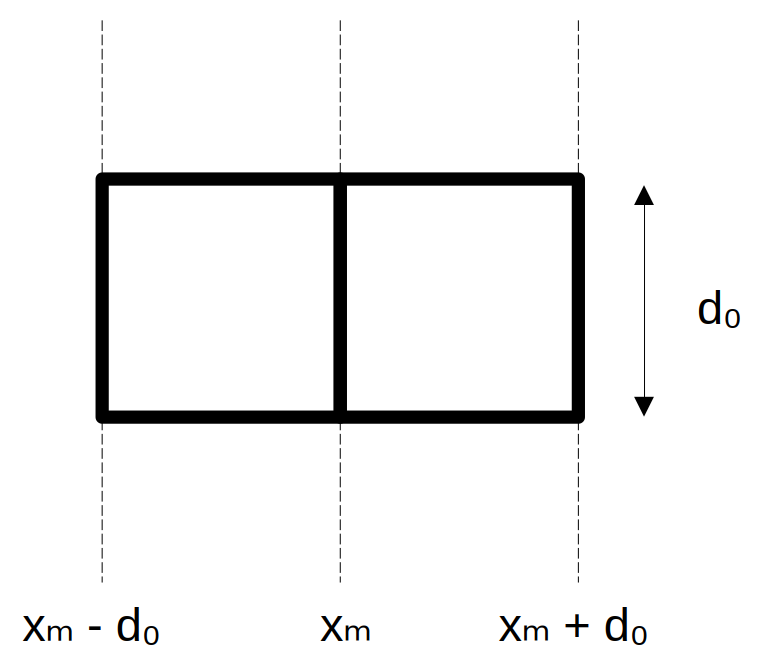
\includegraphics[width=\linewidth]{lecon/13-D&R/7_points.png}
\end{minipage}
\qquad
\begin{minipage}{0.5\linewidth}
	On a au plus 8 éléments dans ce rectangle, car dans chaque domaine, les points sont au moins à distance $d_0$. On a donc au plus $4$ points par carré, d'où le résultat en mettant notre point sur le bas du rectangle.
\end{minipage}

\begin{proposition}
	On a une complexité en $O\left(n (\log n)^2\right)$
\end{proposition}




\subsection{Arbre K-dimensionnel}

\textbf{Problème :} Trouver les $k$ plus proches voisins d'un point $y \in \mathbb R^K$ parmi un ensemble de $n$ points $x_1, \dots, x_n \in \mathbb R^K$

\textbf{Solution initiale :} Stocker nos $k$ valeurs en cours dans une file de priorité et parcourir les n points, en mettant à jour la file de priorité. $\to O(n \log k)$

\begin{algo}[Solution D\&R]
	Faire un pré traitement où l'on stockera nos valeurs dans un arbre binaire de recherche, où l'on partitionnera récursivement les données alternativement sur chaque dimension. La recherche se fait alors en ne cherchant que d'un côté si le deuxième n'est pas nécessaire.
\end{algo}

\textbf{Développement :} Présentation de la structure d'arbre K-dimensionnel

\begin{proposition}[Complexité]\enspace
	\begin{itemize}
		\item prétraitement : $O(n \log(n))$
		\item Recherche des $k$ plus proches voisins : $O(\log n \times k)$ en moyenne, $O(N \times K)$ dans le pire des cas
	\end{itemize}
\end{proposition}


\begin{rem}
	On y perd pour une seule recherche, mais si on cherche les $k$-plus proches voisins de $N$ points, on obtient du $O(n \log n + N \times k \times \log n)$ au lieu de $O(N \times n \times \log k)$.
\end{rem}

\begin{com}
	Si il reste beaucoup de places ou si on veut enlever un exemple au dessus (comme le tri rapide faisant doublons avec le tri fusion, même si il est très classique), on peut rajouter une section supplémentaire ici, et parler de l'additionneur à retenue anticipée par méthode D\&R du développement *à compléter*
\end{com}	

\chapter{Programmation dynamique} \label{L14}
\dev{Emile Martinez}{}

\begin{com}
	On présentera d'abord le principe de la méthode diviser pour régner. Ensuite on divise nos exemples, en deux : ceux qu'on verrait dans la leçon diviser pour régner car ils sont là spécifiquement pour illustrer le paradigme, et ceux que l'on verrait au cours de l'année, et s'appuyant sur le fait qu'on ait déjà vu la méthode diviser pour régner. Cette distinction vient du fait que dans un vrai cours, on ferait comme ça, et les problèmes de la dernière partie serait insérer dans autre chose, et on souligne alors le fait que on ne ferait pas simplement une liste d'algo, mais que pour que le paradigme soit assimiler, il faut mieux le présenter et y revenir régulièrement, plutôt que d'introduire plusieurs fois beaucoup de concepts. (et on met ainsi de la structure sans faire simplement une liste)
\end{com}

\section{Principe}

\subsection{Motivation}

\begin{algo}
	Implémentation naïve de la suite de Fibonacci\\
	\begin{algorithm}[H]
		\caption{$fibo(n)$}
		\eSi{$n = 0$ ou $n = 1$}
			{\Retour{$n$}}
			{\Retour{$fibo(n-1) + fibo(n-2)$}}
	\end{algorithm}
\end{algo}

\begin{proposition}
	Complexité en $O(2^n)$
\end{proposition}

Graphe des dépendances des sous problèmes pour $n = 5$

\begin{minipage}{0.3\linewidth}
	\begin{tikzpicture}[->, node distance=2cm]
		\node[state] (q0) {$F_5$};
		\node[state, below left of = q0] (q1) {$F_3$};
		\node[state, below right of =q0] (q2) {$F_4$};
		\node[state, below of =q1] (q3) {$F_1$};
		\node[state, below of =q2] (q4) {$F_2$};
		\node[state, below right of=q3] (q5) {$F_0$};
		
		\draw (q0) edge[] (q1);
		\draw (q0) edge[] (q2);
		\draw (q2) edge[] (q1);
		\draw (q1) edge[] (q3);
		\draw (q1) edge[] (q4);
		\draw (q2) edge[] (q4);
		\draw (q4) edge[] (q3);
		\draw (q4) edge[] (q5);
		
	\end{tikzpicture}
\end{minipage} \qquad
\begin{minipage}{0.6\linewidth}
	Les sous-problèmes se chevauchent : la méthode diviser pour régner est inefficace.\\\\
	En programmation dynamique, on stocke les valeurs des sous-problèmes pour éviter de recalculer.
\end{minipage}

\begin{algo}
	\label{14-fibo2}
	Fibonacci avec stockage.\\
	\begin{algorithm}[H]
		\caption{$Fibo(n)$}
		$F \gets [0, 1]$\\
		\Pour{$i$ allant de $2$ à $n$}
			{Ajouter $F[i-1] + F[i-2]$ à $F$}
		\Retour{$F[n]$}
	\end{algorithm}
\end{algo}

\subsection{Définition}

\begin{definition}
	La programmation dynamique consiste à résoudre un problème en le décomposant en sous-problèmes, puis à résoudre les sous-problèmes, des plus petits aux plus grands en stockant les résultats intermédiaires.
\end{definition}

\begin{principe}
	\enspace
	\begin{enumerate}
		\item Complexifier le problème en créant plein de sous-problèmes (dont un sera celui que l'on veut résoudre)
		\item Trouver une relation entre les sous-problèmes
		\item Résoudre les sous-problèmes en partant du plus petit, en utilisant la relation :\begin{itemize}
			\item Soit impérativement en ayant un tableau des sous-problème qui stockera leur résultat, et en le remplissant avec une (ou des) boucle (méthode ascendante)
			\item Soit récursivement en mémoïsant. (méthode descendante)
		\end{itemize}
		
	\end{enumerate}
\end{principe}

\begin{rem}
	L'algorithme \ref{14-fibo2} utilise la méthode ascendante. On aurait pu utiliser uniquement deux variables et écraser les résultats intermédiaires.
\end{rem}

\begin{rem}
	Dans le paradigme diviser pour régner, les sous pb sont indépendants. On peut donc se passer de la mémoïsation.
\end{rem}

\begin{rem}
	Pour obtenir, en plus de la valeur de la solution optimale, quelle est cette solution, on peut mémoriser quel(s) sous-problème(s) on a utilisé pour l'obtenir.
\end{rem}

\textbf{Développement :} Illustration du paradigme sur le problème du chemin dans la pyramide.

\section{Algorithmes illustrant le principe}

\subsection{Rendu de monnaie}

\textbf{Instance :} $n$ pièces $p_1, ... p_n$, $S \in \N$

\textbf{Pb :} trouver un $n$-uplet $T = (x_1,  \dots, x_n) \in \N^n$ te que $\sum\limits_{i = 1}^n x_i p_i = S$ et qui minimise $\sum\limits_{i = 1}^n x_i $.
(i.e. trouver le nombre de pièces minimum pour rendre la monnaie)

\begin{algo}
	Approche gloutonne : \begin{enumerate}
		\item Ajouter la pièce $p_i$ de plus grande valeur $\leq S$
		\item Recommencer avec $S -p_i$
	\end{enumerate}
\end{algo}

Cet algorithme est-il optimal ?
\begin{exercise}
	Avec les pièces $(4, 3, 1)$, trouver une somme $S$ pour laquelle le glouton n'est pas optimal ($S = 6$ convient)
\end{exercise}

\begin{algo}[Approche par programmation dynamique du rendu de monnaie]
	\enspace
	\begin{enumerate}
		\item On considère les sous-problèmes $R(s)$ pour $s \in \llbracket 0, S \rrbracket$
		\item Pour trouver la relation de récurrence, on regarde la dernière pièce rendue $p_i$. On a alors $$R(S) = \left\{ \begin{array}{ll}
			+\infty & \text{si } S<0\\
			0 & \text{si } S = 0\\
			\min\limits_{i\in \{1, \dots, n\}} (R(s-p_i)+1) &\text{sinon}
		\end{array}\right.$$
		\item Résolution des sous problèmes (méthode descendante)\\
		\begin{algorithm}[H]
			\caption{$rendu(P, S, m)$}
			\Entree{$P$ est un tableau tel que $P[i] = p_i$}
			\multientree{$m$ tableau de mémoïsation initialisé à 0}
			\Si{$S = 0$}
				{\Retour{0}}
			\Si{$m[S] > 0$}
				{\Retour{$m[s]$}}
			$n \gets +\infty$\\
			\Pour{$p \in P$}
				{$n \gets \min(n, 1+rendu(P, S-p, m))$}
			$m[S] \gets n$\\
			$\Retour{n}$
		\end{algorithm}
	\end{enumerate}
	Complexité : $O(n\times S)$
\end{algo}

\begin{exercise}
	Écrire la méthode ascendante de résolution (i.e. trouver l'ordre de remplissage du tableau)
\end{exercise}

\subsection{Sac à dos}

\textbf{Instance :} $n$ objets de poids $\{w_1, \dots, w_n\} \in \N^n$, et de valeur $\{v_1, \dots, v_n\}\in \N^n$. Une capacité $W \in \N$.
\textbf{Problème :} Trouver $T = (x_1, \dots, x_n) \in \{0, 1\}^n$ tel que $\sum\limits_{i = 1}^n x_iw_i \leq W$ et qui maximise $\sum\limits_{i=1}^n w_iv_i$

\begin{exercise}
	Proposer des algorithmes gloutons pour résoudre le pb du sac à dos. Sont-ils optimaux ?
\end{exercise}

\begin{algo}[Approche par programmation dynamique du problème du sac à dos]
	\enspace
	\begin{enumerate}
		\item On considère les sous-problèmes $SD(i,w)$ réduit aux $i$ premiers objets avec une capacité $w$. La solution qui nous intéresse est celle de $SD(n, W)$
		\item $T(i, w)= \left\{ \begin{array}{l}
			0 \text{ si } i = 0 \text{ ou } w = 0\\
			\max\Big( \underset{\substack{\text{si l'optimal prend}\\\text{pas l'objet }i}}{\underbrace{T(i-1, w)}} \,,\, \underset{\substack{\text{si l'optimal prend}\\\text{l'objet }i}}{\underbrace{T(i-1, w-w_i) + v_i}} \enspace \Big) \text{ sinon}
		\end{array} \right.$
		\item On remplit à $i$ et $w$ croissant.
	\end{enumerate}
\end{algo}

\begin{rem}
	Le problème de décision associé au problème de sac à dos est NP-complet. Ici, l'algorithme résout le problème d'optimisation en $O(S\times n)$, or la taille de l'instance d'entrée est en $\log|S| + n$, donc notre algorithme n'est pas polynomial en la taille de l'instance.
\end{rem}

\section{Autres applications}

\subsection{L'algorithme de Floyd-Warshall}
\textbf{Instance :} Un graphe orienté $G = (S, A)$ sans circuit absorbant et une fonction de poids $w : A \to \mathbb Z$
\textbf{Problème :} Déterminer les valeurs des plus courts chemins entre toutes les paires de sommets de $G$

\begin{algo}[Résolution du problèmes des plus courts chemins en découpant selon les sommets que l'on utilise]
	\begin{enumerate}
		\item On numérote les sommets de $G$ : $S = \{1, \dots, n\}$. On s'intéresse aux sous problèmes $FW(i,j,k)$ qui correspond au plus court chemin de $i$ à $j$ empruntant des sommets intermédiaires dans $\{1, \dots, k\}$. Les problèmes qui nous intéressent sont $FW(i,j,n)$ pour $i \neq j$.
		\item $FW(i, j, k) = \left\{ \begin{array}{l}
			w(i,j) \text{ si } k = 0\\
			\min \Big( \underset{\substack{\text{si le plus court}\\\text{chemin de $i$ à $j$}\\\text{n'utilise pas } k}}{\underbrace{F(i,j, k-1)}} \, , \, \underset{\substack{\text{si le plus court}\\\text{chemin de $i$ à $j$}\\\text{utilise } k}}{\underbrace{F(i,k, k-1)} + F(k, j, k-1)} \Big) \text{ sinon}
		\end{array}\right.$
		\item Résolution par la méthode ascendante\\
		\begin{algorithm}[H]
			\caption{$Floyd-Warshall(G)$}
			$W \gets$ matrice d'adjacence de $G$\\
			\Pour{$k$ allant de $1$ à $n$}
			{
				\Pour{$i$ allant de $1$ à $n$}
					{
						\Pour{$j$ allant de $1$ à $n$}
							{
								$W[i,j] \gets \min (W[i,j], W[i,k] + W[k,j])$
							}
					}
			}
		\end{algorithm}
	\end{enumerate}
	Complexité : $O(|S|^3)$
\end{algo}

\begin{rem}
	On écrase la matrice au fur et à mesure car l'étape $k$ ne dépend que de l'étape $k-1$
\end{rem}

\begin{rem}
	On aurait pu découper les sous problèmes différemment. Par exemple, on peut découper au chemin de taille au plus $k$. On retombe alors sur un algorithme de routage en réseau.
\end{rem}

\textbf{Développement :} Terminaison et discussion autour de l'algorithme de Bellman-Ford

\subsection{Distance de Levenshtein (d'édition)}

\begin{definition}
	La \textbf{distance de Levenshtein} correspond au nombre minimum d'opérations (suppression, modification ou ajout d'une lettre) pour transformer un chaîne de caractère en l'autre.\\
	
	Plus formellement, pour $a \in \Sigma$, $i \in \N$ on définit
	\begin{itemize}[label=$\star$]
		\item $ins_{a, i} : \Sigma^* \to \Sigma^*$ : insertion de la lettre $a$ à la position $i$
		\item $sub_{a, i} : \Sigma^* \to \Sigma^*$ : modification de la lettre à la position $i$ en $a$
		\item $sup_{i} : \Sigma^* \to \Sigma^*$ : suppression de la lettre à la position $i$
	\end{itemize}
	et alors $lev(w_1, w_2) = \min\Big\{ k \in \N \quad \big/ \quad \exists f_1, \dots, f_k \in \{ins_{a,i}, sub_{a,i}, sup_i / a\in \Sigma, i \in \N \} : w_2 = f_k \circ \dots \circ f_1 (w_1) \Big\}$ 
\end{definition}

\begin{exercise}
	C'est une distance.
\end{exercise}

\begin{com}
	Ici on ne donne que l'idée parce que on a pas la place et parce que l'élève peut avoir le recul pour trouver lui-même
\end{com}
\begin{algo}[Idée de l'approche par programmation dynamique pour la distance de levenshtein]
	\begin{enumerate}
		\item Considérer la distance d'édition entre tous les préfixes de $w_1$ et $w_2$
		\item Considérer la modification sur la dernière lettre (rien, insertion, suppression ou modification)
		\item Résoudre à préfixe croissant
	\end{enumerate}
\end{algo}

\chapter{Exemples d’algorithmes d’apprentissage supervisés et non supervisés} \label{L15}
\dev{Emile Martinez}{}

\section{Introduction}

\subsection{Définition}

\begin{definition}
	On dit que un algorithme apprend via un entraînement pour un ensemble de tâches et une mesure de performance si sa performance sur les tâches mesuré par la mesure de performance s’améliore après l'entraînement.
\end{definition}

\begin{definition}
	\label{15-def-1}
	On considère deux familles de l’apprentissage machine :
	\begin{enumerate}
		\item l’apprentissage supervisé : on dispose d’espaces $X$ d’entrée et $Y$ de sortie, et d’un ensemble $E$ d’exemples $(x_i , y_i ) \in X \times Y$, représentant une fonction $f : X \to Y$. Le but étant alors de construire une fonction $\hat{h} : X \to Y$ approximant $f$.
		\item l’apprentissage non supervisé : on dispose seulement de l’espace $X$  dont on veut alors découvrir les structures sous-jacente
	\end{enumerate}
\end{definition}

\begin{example}
	Sur un ensemble de données sur des animaux, on peut :\begin{enumerate}
		\item Savoir lesquels sont des chiens, des chats, etc... (apprentissage supervisé)
		\item Savoir quels animaux sont de la même espèce (apprentissage non supervisé)
	\end{enumerate}
\end{example}

\begin{rem}
	Il existe d’autres familles, comme l’apprentissage par renforcement qui consiste à maximiser un critère d’utilité par expériences successives.
\end{rem}

\subsection{Évaluation d'un algorithme d'apprentissage}
\label{15-I-2}

On cherche à évaluer la performance d'un algorithme d'apprentissage.

\begin{definition}
	On découpe nos données d'entrées $E$ en deux :
	\begin{itemize}
		\item Les données d'apprentissage, servant à entraîner l'algorithme
		\item Les données de validation, servant à imiter la prédiction, mais en comparant le résultat obtenu à celui attendu.
	\end{itemize}
\end{definition}

\begin{rem}
	Si l'on a trop peu de données, on peut également faire une validation croisée, consistant utiliser alternativement des données comme apprentissage et comme validation
\end{rem}

\begin{rem}
	Cette phase est également utile pour calibrer les paramêtres de l'algorithme.
\end{rem}

\section{Apprentissage supervisé}

On reprend les notations de la définition \ref{15-def-1}

\begin{com}
	Dans un vrai cours, on réécrirait les définitions pour plus de clarté
\end{com}

\begin{definition}\enspace
	
	Si $Y$ est un ensemble fini de classes, on parle de problème de classification.
	
	Si $Y =\mathbb R$, on parle de problèmes de régression.
\end{definition}

\begin{example}
	Sur un ensemble de données sur des animaux, on peut avoir : \begin{itemize}
		\item $Y = \{'chien', 'chat'\}$ (classification)
		\item $Y = \mathbb R$ représentant le poids de l'animal (régression)
	\end{itemize}
\end{example}

Concentrons nous sur le problème de classification. On cherche à inférer de $E$, la classe de $\alpha \in X$. Notons $C$ la partition de $X$ représentant les différentes classes.

\subsection{$K$ plus proches voisins}

On s'intéresse ici au cas où $X = \mathbb R^d$

\begin{algo}
	K plus proches voisins de $\alpha$
	\begin{enumerate}
		\item Déterminer les $K$ plus proches voisins de $\alpha$ dans $E$
		\item Choisir la classe majoritaire parmi ces voisins.
	\end{enumerate}
\end{algo}

\textbf{Développement :} Présentation de l'algorithme illustrant différents aspects de l'apprentissage machine.

\begin{example}\enspace\\
	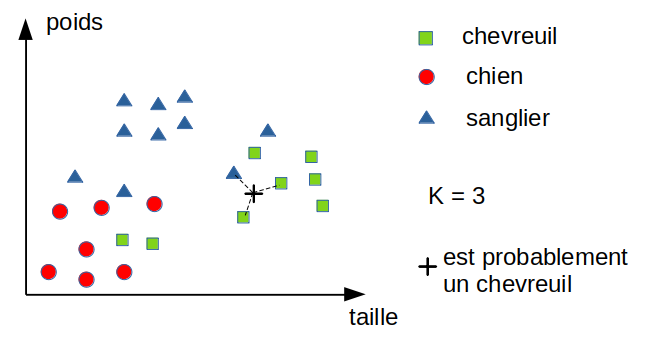
\includegraphics[width=0.6\linewidth]{lecon/15-ml/graphe.png}
\end{example}

\begin{rem}
	Ici pour choisir k, on utilise la méthode de mesure de performance du \ref{15-I-2} en essayant plusieurs paramètres.
\end{rem}

\begin{exercise}
	Appliquer l'algorithme sur le jeu de données MINST.
\end{exercise}

\begin{rem}
	Pour un problème de régression, on ne choisirait pas la classe majoritaire à l'étape 2, mais on agrégerait les données (par exemple en faisant une moyenne).
\end{rem}

\begin{impl}\enspace
	
	\textbf{Solution initiale :} Stocker nos $K$ valeurs en cours dans une file de priorité (implémentée par un tas max) et parcourir les $n$ points en mettant à jour la file de priorité
	
	\textbf{Complexité :} $O(n\log k)$\\
	
	\textbf{Solution diviser pour régner :} Faire un pré traitement où l'on stockera nos valeurs dans un arbre binaire de recherche (arbre $d$-dimensionnel), où l'on partitionnera récursivement les données alternativement sur chaque dimension. La recherche se fait alors en ne cherchant que d'un côté si le deuxième n'est pas nécessaire.
	
	\textbf{Complexité :}\\
	Prétraitement :$O(n \log n)$\\
	Recherche des k voisins : $O(k \log n)$ en moyenne et $O(nk)$ dans le pire des cas.
\end{impl}

\noindent \textbf{Développement :} Présentation de la structure d'arbre $d$-dimensionnel.

\begin{rem}
	On parle souvent d'arbre $k$-dimensionnel, mais on prend ici $d$ pour éviter la confusion avec $K$.
\end{rem}

\subsection{Arbre de décision}

On s'intéresse ici au cas $X = \mathbb R^d$ (ou $\{O, 1\}^d$)

\begin{idee}
	Partitionner récursivement X grâce à un arbre de décision où chaque feuille a une classe.\\
	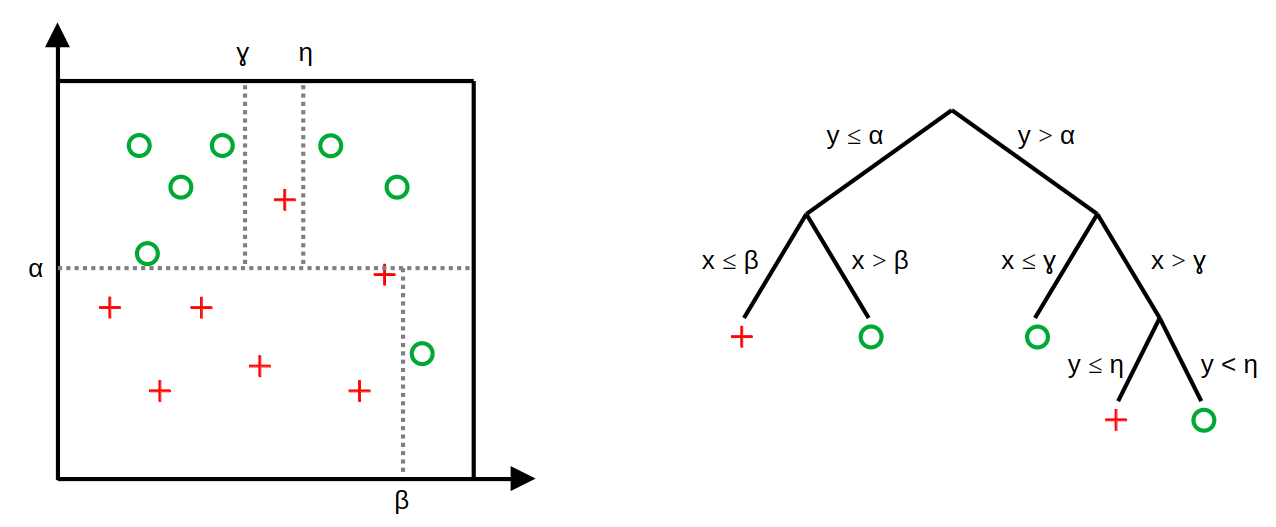
\includegraphics[width=\linewidth]{lecon/15-ml/arb_dec.png}
\end{idee}

\begin{definition}
	Définissons l'entropie d'une partie $S$ de $E$ : $H(S) = \sum\limits_{c \in C} \dfrac{|S\cap c|}{|S|} \times \log\left(\dfrac{|S\cap c|}{|S|}\right)$
\end{definition}

\begin{rem}
	Si tous les éléments ont la même classe, $H(S) = 0$
\end{rem}

\begin{definition}
	Le gain d'une partition $S_1$, $S_2$ de $S$ est : $$H(S) - \left( \dfrac{|S_1|}{|S|} \times H(S_1) + \dfrac{|S_2|}{|S|} \times H(S_2) \right)$$	
\end{definition}

\begin{algo}
	On construit récursivement notre arbre de décision sur notre ensemble S de données restantes:
	\begin{itemize}[label=$\bullet$]
		\item Si $S$ est vide : Choisir la classe la plus représentée du nœud parent
		\item Si toutes les données de $S$ ont la même classe : en faire une feuille avec cette classe.
		\item Sinon, on choisit la coordonnée $i$ et la valeur $m$ tel que la partition $$ S_1 = \left\{ (x_1, \dots, x_n) \in S / x_i \leq m\right\} \text{ et } S_2 = \left\{ (x_1, \dots, x_n) \in S / x_i > m\right\}$$ maximise le gain
	\end{itemize}
\end{algo}

\begin{rem}
	On atteint très vite du sur apprentissage. Pour éviter cela, on peut élaguer le bas de l'arbre (algorithme de Cart)
\end{rem}

\begin{exercise}
	Application à détecter la langue d'une page wikipedia à partir de la matrice de fréquence de facteurs de 2 lettres.
\end{exercise}

\begin{com}
	Ici pour ce TD, on peut mentionner à l'oral le fait qu'on peut utiliser ce truc pour de vrais, et surtout que on peut éventuellement faire réfléchir les élèves à comment modéliser le problème. Fréquence des mots, KNN avec distance de levenstein, fréquence des facteurs de 1, 2, 5 lettres ? Ce qui rend tout ca très intéressants selon moi. (suivant le nombre de pages en exemples, on peut prendre les facteurs d'un certain nombres de lettres (on aura un tableau de taille $27^{\text{taille des facteurs}}$) et ensuite faire du KNN, de l'arbre de décision, etc...) (Avec 4000 pages par langues pour 13 langues, et les facteurs de 2 mots, on classifie très bien).
\end{com}

\begin{rem}
	Dans le cas d'une régression, on peut prendre comme mesure d'impureté la variance.
\end{rem}

\subsection{Représentation de la qualité des classes}

Quand on mesure la performance de notre algorithme on peut chercher à représenter la qualité de nos prédictions (pour classification).

\begin{definition}[matrice de confusion]
	On associe $Y$ à $\{1, \dots, n\}$. La matrice de confusion est alors la matrice carrée $M$ de taille $n$ tel que $M_{i,j}$ est le nombre d'éléments de la classe $i$ qui ont été classés à $j$
\end{definition}

\begin{proposition}
	Plus notre algorithme est correcte, plus la diagonale est dominante.
\end{proposition}

\section{Apprentissage non supervisé}

\begin{rem}
	Il existe plusieurs types d'apprentissage non supervisé. On peut par exemple penser à la réduction de dimension : On a $X\subset \mathbb R^n$ et on cherche $f : X \to \mathbb R^m$ avec $n < m$ et tel que $f(x)$ et $f(y)$ sont proches si $x$ et $y$ le sont aussi.
	
	On se concentrera sur ce qu'on appellera regroupement, (clustering en anglais, ou classification non supervisée) qui consiste à trouver $f : X \to \{1, ..., k\}$ essayant de regrouper les éléments les plus proches.
\end{rem}

\begin{example}
	On a un manuscrit dans un alphabet inconnu, et on cherche à savoir quels lettres sont les mêmes.
\end{example}

\begin{exercise}
	Dans l'exemple au dessus, quel $X$ prendre ?
\end{exercise}

\subsection{Classification hiérarchique ascendante}

\begin{idee}
	Chacun est seul dans sa classe au début, et tant qu'on a $k$ classes, on fusionne les classes les plus proches.
\end{idee}

\begin{rem}
	C'est un algorithme glouton
\end{rem}

\begin{rem}
	Pour définir la distance entre deux classes, on prendre prendre : \begin{itemize}[label=$\bullet$]
		\item $d(S_1, S_2) = \min\limits_{x \in S_1, y \in S_2} (d(x, y))$
		\item $d(S_1, S_2) = \min\limits_{x \in S_1, y \in S_2} (d(x, y))$
		\item $d(S_1, S_2)  = \dfrac{1}{|S_1| \times |S_2|} \sum\limits_{x \in S_1, y \in S_2} d(x, y)$
	\end{itemize}
\end{rem}

\begin{exercise}
	Activité : Représenter l'exécution de l'algorithme sur un dendrogramme
\end{exercise}

\subsection{ALgorithme des $k$-moyennes}

\begin{idee}
	On cherche à trouver $S_1, \dots, S_k$ une partition de $X$ et $z_1, \dots, z_k \in \mathbb R^d$ minimisant $\sum\limits_{i = 1}^{k} \sum\limits_{x \in S_i} d(x, z_i)$
\end{idee}

\begin{algorithm}
	\caption{K-mean}
	Assigner à chaque valeur une classe aléatoire\\
	\Repeter{stabilisation}
	{
		\Pour{$x \in X$}
		{
			assigner à $x$ la classe de $\argmin\limits_{i \in \{1, \dots, k\}} d(x, z_i)$
		}
		\Pour{$i$ allant de $1$ à $k$}
		{
			$z_i \gets \dfrac{1}{|S_i|} \sum\limits_{x \in S_i} x$
		}
	}	
\end{algorithm}

\begin{proposition}
	Cet algorithme termine
\end{proposition}

\begin{proof}
	La cible diminue à chaque étape, et ne peut prendre qu'un nombre fini de valeurs.
\end{proof}

\begin{rem}
	On ne trouve pas toujours le minimum, on tombe souvent dans un minimum local. On relance alors plusieurs fois l'algorithme (d'où l'aléatoire au début).
\end{rem}

\begin{exercise}
	TP sur la réduction de palette d'une image
\end{exercise}

\begin{rem}
	Comment choisir $k$ ? Pour la classification hierarchique ascendante, on s'arrête au plus grand saut sur le dendrogramme, pour les k-moyennes, on affiche la cible finale en fonction de $k$ , et on choisit $k$ au changement de pente.
\end{rem}

\begin{com}
	Bon la faudrait faire les deux dessins mais à très court terme j'ai la flemme.
\end{com}

\chapter{Exemples d'algorithmes pour l'étude des jeux} \label{L16}
\dev{Emile Martinez}{}

La théorie des jeux s'intéresse aux interactions entre des individus (joueurs) qui effectuent des choix selon les règles d'un jeu.

\section{Jeux d'accessibilité à deux joueurs}

\subsection{Définition}

\paragraph{Notation :} Pour $G = (S, A)$, on note $Fin(G) = \{v \in S / deg^+(v) = 0\}$

\begin{definition}
	\label{16-def-jeu}
	Un jeu à deux joueurs est :\begin{itemize}
		\item une arène : un graphe orienté biparti $G = (S_1 \sqcup S_2, A)$
		\item un sommet de départ $s_0$
		\item une partition de $Fin(G) = G_1 \sqcup G_2 \sqcup N$
	\end{itemize}
\end{definition}

\begin{com}
	On peut mentionner ici qu'on peut se restreindre au graphes bipartie, car si quand on joue, c'est à nouveau à nous, on considère les deux coups à jouer d'affilée comme un seul. Mais y a des jeux où on peut rejouer, il faut alors travailler un peu pour modéliser.
\end{com}

\begin{idee}
	Les sommets de $S_1$ sont ceux où J1 joue. Un arc $x \to y$ représente un coup possible pour le joueur qui contrôle l'état $x$, qui déplace alors le jeu dans l'état $y$. $G_i$ sont les états gagnants pour Ji, $N$ ceux d'une partie nulle.
\end{idee}

\begin{example}
	Représentation d'un échantillon de la modélisation du Tic-Tac-Toe\\
	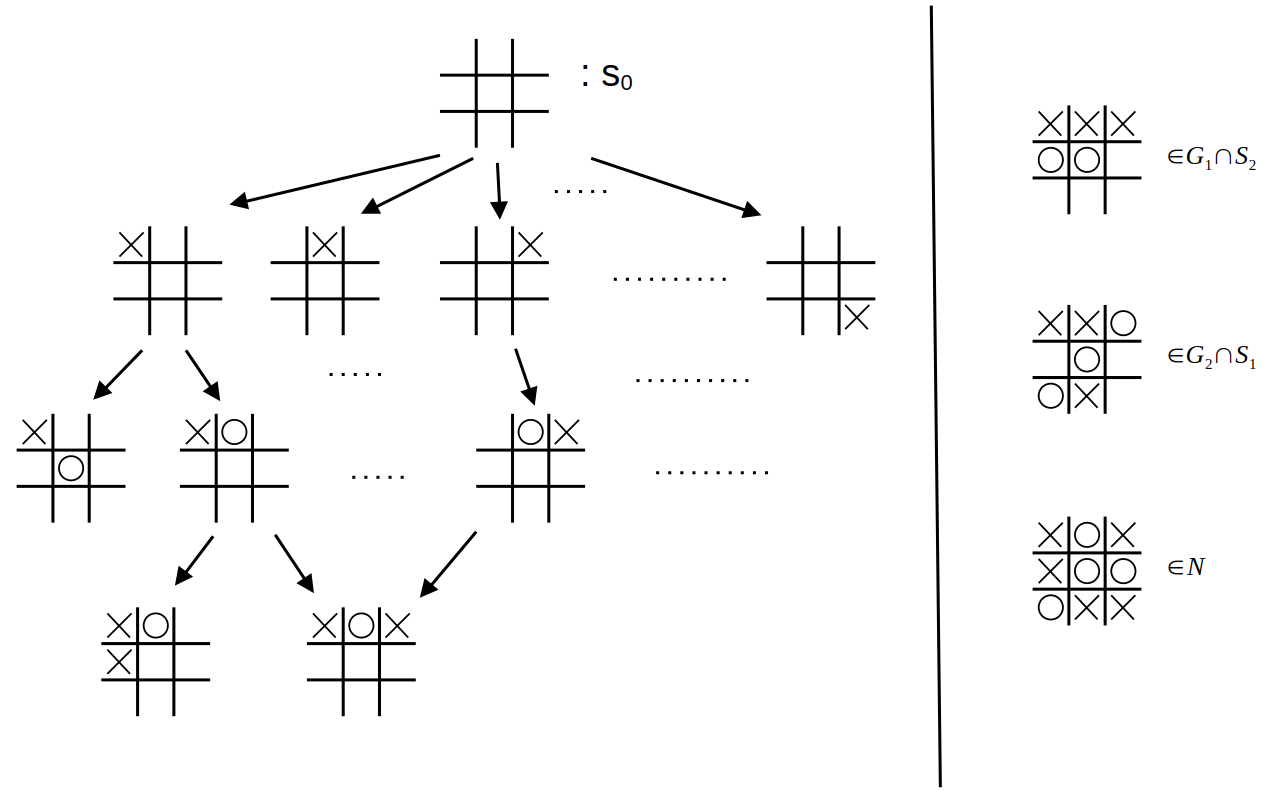
\includegraphics[width=\linewidth]{lecon/16-jeu/tic-tac-toe.png}
\end{example}

\begin{definition}[Partie]
	Une partie d'un jeu $(G, s_0, G_1, G_2, N)$ est un chemin de $s_0$ à un sommet $s_f \in Fin(G)$.
\end{definition}

\begin{definition}
	On appelle stratégie pour le joueur $i \in \{1, 2\}$ toute fonction $\varphi : V_i \to V$ tel que $\forall u \in V_i \backslash Fin(G), \, (u, \varphi(u)) \in A$.
\end{definition}

\begin{com}
	Ici on définit directement une stratégie sans mémoire, le programme se limitant à cela, et les jeux que nous considérerons ne nécessitant pas de stratégie avec mémoire.
\end{com}

\begin{definition}[Stratégie gagnante]
	$\varphi$ est une stratégie gagnante pour le joueur $i$ si pour toute partie $P = s_0, \dots, s_f$,
	$$ \Big( \forall j \in \llbracket O, f-1 \rrbracket, s_j \in V_i \implies s_{j+1} = \varphi(s_j) \Big) \implies s_f \in G_i$$
	$s$ est une position gagnante s'il existe une stratégie gagnante depuis $s$.
\end{definition}

\begin{idee}
	$\varphi$ est une stratégie gagnante si quand les coups de Ji sont ceux de $\varphi$, alors Ji gagne indépendamment de ce que joue l'autre joueur. 
\end{idee}

\subsection{Attracteurs}

On se place du point de vue du joueur 1, mais la situation est symétrique avec le joueur 2.

\begin{definition}[Attracteur]
	Pour une arène $(G, s_0)$, et $F \subset V$ on note $Attr_i(F)$, l'ensemble des sommets depuis lesquels le joueur J1 a une stratégie pour arriver dans $F$ en au plus $i$ étapes. On note $Attr(F) = \bigcup\limits_{i = 0}^{+\infty} Attr_i(F)$
\end{definition}

\begin{proposition}
	Pour un jeu $(G, s_0, G_1, G_2, N)$, $Attr(G_1)$ est l'ensemble des position gagnante de J1.
\end{proposition}

\begin{proposition}\enspace
	\begin{itemize}[label=$\bullet$]
		\item $Attr_0(F) = F$
		\item $Attr_{i+1}(F) = Attr_i(F) \: \cup \: \{u \in V_1 \, / \, \mathcal N^+(u) \cap Attr_i(F) \neq \emptyset\} \: \cup \: \{u \in V_2 \, / \, \mathcal N^+(u) \subset Attr_i(F)\} $
	\end{itemize}
\end{proposition}

\begin{proposition}
	Si $G$ est fini alors $\left( Attr_i(F) \right)$ est croissante bornée, donc stationnaire. Sa limite est alors $Attr(F)$.
	
	Une stratégie gagnante depuis $Attr(F)$ est :
	$$ \begin{array}{rcl}
		\varphi : V_1 & \to V\\
		v & \mapsto & \left\{ \begin{array}{ll}
			\omega \in \mathcal N^+(v) \cap Attr_i(F) & \text{si } v \in Attr_{i+1}(F) \backslash Attr_i(F)\\
			\omega \in \mathcal N^+(v) & \text{si } v \notin Attr(F)
		\end{array} \right.
	\end{array} $$
\end{proposition}

\paragraph{Développement :} Stratégies gagnantes pour le jeu de Nim à 1 puis plusieurs tas.

\section{Jeux Min-Max}

\subsection{Algorithme Min-Max}

On considère ici des jeux à deux joueurs, en reprenant la définition \ref{16-def-jeu} en  remplaçant la partition de $Fin(G)$ par une fonction de coût $c : Fin(G) \to \mathbb Z$.

Le joueur 1 (appelé Max ici) essaye alors de maximiser par ses coups la valeur finale, et le joueur 2 (ici Min) essaye de la minimiser.

\begin{rem}
	La partie précédente en est un cas particulier avec $c(G_1) = 1$, $c(N) = 0$ et $C(G_2) = 1$ 
\end{rem}

\begin{definition}
	Une stratégie optimale pour le joueur Max (resp. Min) est une stratégie maximisant (resp. minimisant) le coût.
\end{definition}

\begin{algo}
	On fait une recherche exhaustive de tous les coups, en prenant à chaque fois celui ayant le résultat maximum (resp.minimimum) quand Max (resp. Min) joue. Cela détermine une stratégie optimale (pour les deux joueurs).
\end{algo}

\begin{rem}
	En pratique, c'est souvent infaisable tant le graphe est gros.
	\begin{example}
		Les echecs, avec +1000 victoire blanche, -1000 victoire noire et 0 nulle, le graphe a plus de $10^44$ sommets.
	\end{example}
\end{rem}

\begin{definition}
	Une heuristique $h : V \to \mathbb Z$ est une estimation de à quoi mènerait dans le meilleur cas cette position
\end{definition}

\begin{com}
	Ici on a une définition formelle avec l'intuition de son interprétation (et donc de son usage). (une heuristique, c'est simplement une fonction $V \to \mathbb Z$)
\end{com}

\begin{example}
	La fonction qui aux échecs donne la somme de la valeur des pièces
\end{example}

\begin{idee}
	On fait l'exploration exhaustive en renvoyant l'heuristique quand on a fait suffisament d'étapes.
\end{idee}

\begin{algorithm}[H]
	\caption{$MinMax(j, prof, u)$}
	\Si{$u \in Fin(G)$ ou $prof = 0$}
		{\Retour{$h(u)$}}
	\eSi{$i == 1$}
		{$f\gets \max$}
		{$f \gets\min$}
	\Retour{$f\Big(\Big\{MinMax(3-j, \,prof-1, \,v) \enspace \big/ \enspace v \in \mathcal N^+(u)\Big\}\Big)$}
\end{algorithm}

\subsection{Élagage $\alpha$-$\beta$}

\begin{minipage}{0.5\linewidth}
	\begin{idee}
		Il n'est pas nécessaire d'explorer tout l'arbre : si je suis Min et que Max au coup d'avant peut faire 5 avec un autre coup, dès que je vois que je peux faire 1, je peux arrêter d'explorer, car je sais que Max ne fera pas ce coup.
	\end{idee}
\end{minipage} \quad \begin{minipage}{0.4\linewidth}
	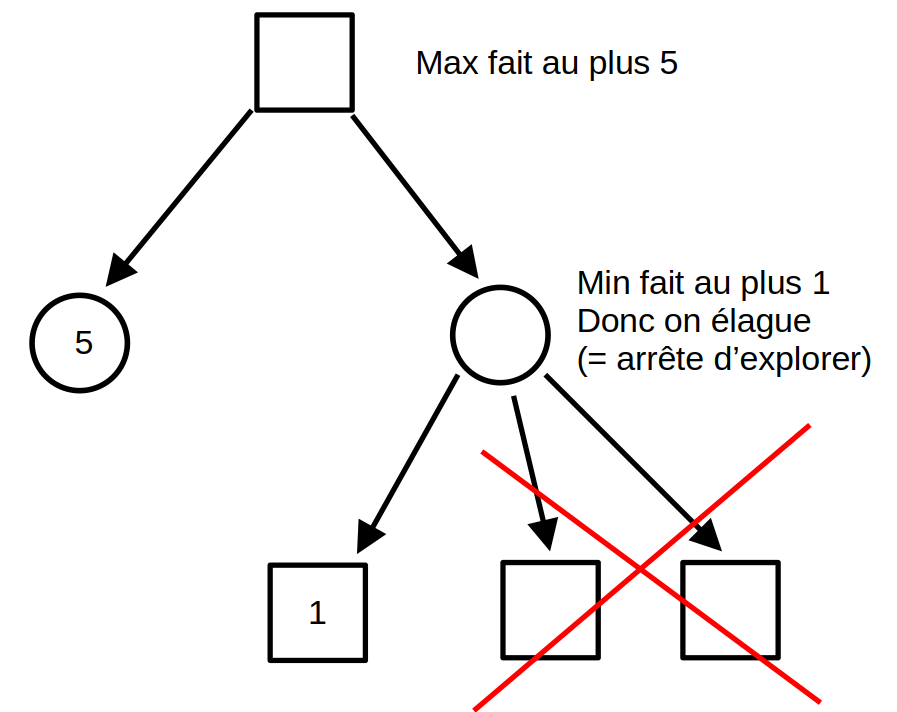
\includegraphics[width=\linewidth]{lecon/16-jeu/alpha_beta.png}
\end{minipage}

\begin{algorithm}[H]
	\caption{$Alphabeta(j, \alpha, \beta, u)$}
	\Si{$u \in Fin(G)$}
		{\Retour{$c(u)$}}
	\eSi{$joueur = 1$}
	{
		$res \gets -\infty$\\
		\Pour{$v$ voisin de $u$}
		{
			$e = Alphabeta(2, \max(res, \alpha), \beta, v)$\\
			\eSi{$e > \beta$}
				{\Retour{$e$}\quad \tcp{Élagage}}
				{$res \gets \max(e, res)$}
		}
		\Retour{$res$}
	}
	{
		\tcp{Symétrique, à faire en exercice}
	}
\end{algorithm}

\begin{idee}
	$\alpha$ (resp. $\beta$) est la valeur maximale (resp. minimale) que peut faire Max (resp. Min) parmi ce que l'on a explorer pour l'instant. (On appelle donc $alphabeta(1, -\infty, +\infty, s_0)$)
\end{idee}

\begin{rem}
	Cet algorithme est exact. On peut, comme pour Min-Max ajouter une profondeur et une heuristique.
\end{rem}

\begin{exercise}
	Comparaison des temps d'exécution de Min-Max et de Alpha-Beta pour le Tic-Tac-Toe (exploration complète sans heuristique).
\end{exercise}

\section{Les Jeux à un joueur}

\subsection{Graphe d'état}

\begin{definition}
	Un graphe d'état est la donnée d'un graphe orienté $G = (S, A)$ pondéré par $c : A \to \N$, d'un état initial $s_0$ et d'un ensemble d'états finaux $F \subset S$
\end{definition}

\begin{rem}
	$S$ représente les configurations d'un jeu à un joueur, $A$ les transitions d'une configuration à une autre en un coup, $c$ le coût de cette transition, et $F$ les configurations gagnantes. 
\end{rem}

\paragraph{Objectif :} Trouver un chemin dans ce graphe entre l'état initial et l'un des états finaux de coût total minimal.

\begin{example}
	Dans le jeu du taquin, les états correspondent aux dispositions possibles du plateau. L'état final est le plateau remis dans l'ordre. Chaque case a un degré sortant inférieur ou égal à 4 qui correspond aux déplacements possibles de la case vide (vers le haut, le bas, à gauche ou à droite). Tous les déplacements ont un coût unitaire.
\end{example}

\begin{rem}
	le graphe d'état est en général trop gros pour être stocké entièrement en mémoire. Il est donc nécessaire de mettre en place des stratégies ou des heuristiques pour orienter la recherche du chemin
\end{rem}

\subsection{L'algorithme A*}

\begin{principe}
	L'algorithme A* est une variante de l'algorithme de Dijkstra pour calculer un plus court chemin entre un sommet initial $s_0$ et un sommet final $s_f$. On visite les sommets par estimation de leur proximité à $s_f$ grâce à une fonction $f$ définie par:
	
	$f(s) = d(s) + h(s)$ où $d(s)$ est le coût d'un plus court chemin entre $s_0$ et $s$ et $h(s)$ i une estimation (heuristique) du coût entre $s$ et $s_f$
\end{principe}

\begin{example}
	dans le cas du taquin, on peut penser aux heuristiques suivantes :
	\begin{itemize}[label=$\bullet$]
		\item nombre de chiffres mal placés 
		\item somme des distances de Manhattan des cases à leur position finale
	\end{itemize}
\end{example}

\begin{algorithm}[H]
	\Entree{W la matrice de poids du graphe;
		h le tableau pour l'heuristique;
		$s_{0}$ et $s_{f}$ les sommets initiaux et finaux}
	\Sortie{la distance d'un plus court chemin de $s_{0}$ à $s_{f}$}
	
	$D \gets$ tableau initialisé à $\infty$\\
	$D[s_{0}] \gets$ 0\\
	$P \gets$ file de priorité vide\\
	Ajouter $(s_{0}, h[s_{0}])$ à $P$\\
	\Tq{$P$ non vide}{
		$(s, \_) \gets$ $extraire(P)$\\
		\Si{$s = s_{f}$}{\Retour{$D[s]$}}
		\Pour{$s'$ successeur de $s$}{
			$c \gets D[s] + W[s, s']$\\
			\Si{$c < D[s']$}{
				$D[s'] \gets c$\\
				Ajouter  $(s', c+h[s'])$ à $P$\\
			}
		}
	}
	\Retour{NonAccessible}
	\caption{Algorithme A*}
\end{algorithm}

\begin{rem}
	Si $h = 0$, on retrouve Dijkstra
\end{rem}

\begin{definition}
	Une heuristique est dite admissible si $\forall u \in S, h(u) \leq d(u)$
\end{definition}

\begin{theorem}[Correction]
	Si $h$ est admissible, alors A* renvoie la distance d'un court chemin de $s_0$ à $s_f$.
\end{theorem}

\begin{definition}
	Une heuristique est dite monotone si $\forall (u,v) \in A, h(u) \leq h(v) + w(u,v)$
\end{definition}

\begin{rem}
	Dans un graphe avec les distances euclidiennes entre nœuds, la distance à vol d'oiseau est une heuristique monotone.
\end{rem}

\begin{proposition}
	Si $h$ est monotone et $h(s_f) = 0$, alors A* est correct ($h$ est admissible) et extrait chaque noeud au plus une fois.
\end{proposition}

\paragraph{Développement :} Démonstration du théorème et de la propriété précédente.

\begin{appl}
	Calcul des itinéraires par un GPS
\end{appl}

\chapter{Algorithmes d'ordonnancement de tâches et de gestion de ressources} \label{L17}
\dev{Emile Martinez}{}

\paragraph{Métaphore filée :} Ordonnancement des tâches dans une cuisine.

\section{Motivation : le système d'exploitation}

\begin{rem}
	Lorsque vous utilisez votre PC, vous éxécutez des dizaines de programmes "en même temps" (lecture de mail, taper au clavier, écouter de la musique...). Pourtant, votre PC a un nombre limité de processeurs.
\end{rem}

\begin{definition}[Execution concurrente et ordonnanceur]
	Le système d'exploitation peut interrompre un processus en cours pour exécuter du code qui lui est propre. Il peut alors, à intervalles réguliers, décider à quelle tâche en cours il rend la main. 
	
	Le rôle de l'ordonnanceur est de choisir le prochain processus à exécuter parmi une liste de processus candidats. 
\end{definition}

%\begin{tikzpicture}[->, node distance=2cm]
%	
%	\node (q0) {};
%	\node[state, right=of q0] (pret) {Prêt};
%	\node[state, right=of pret] (elu) {Élu};
%	\node[state, below right=of pret] (blo) {Bloqué};
%	\node[state, right of= elu] (term) {Terminé};
%	
%	\draw (q0) edge[] (pret);
%	\draw (pret) edge[bend left] (elu);
%	\draw (elu) edge[bend left] (pret);
%	\draw (elu) edge[bend left] (blo);
%	\draw (blo) edge[bend left] (pret);
%	\draw (elu) edge[] (term);
%	
%	
%\end{tikzpicture}

\begin{center}
	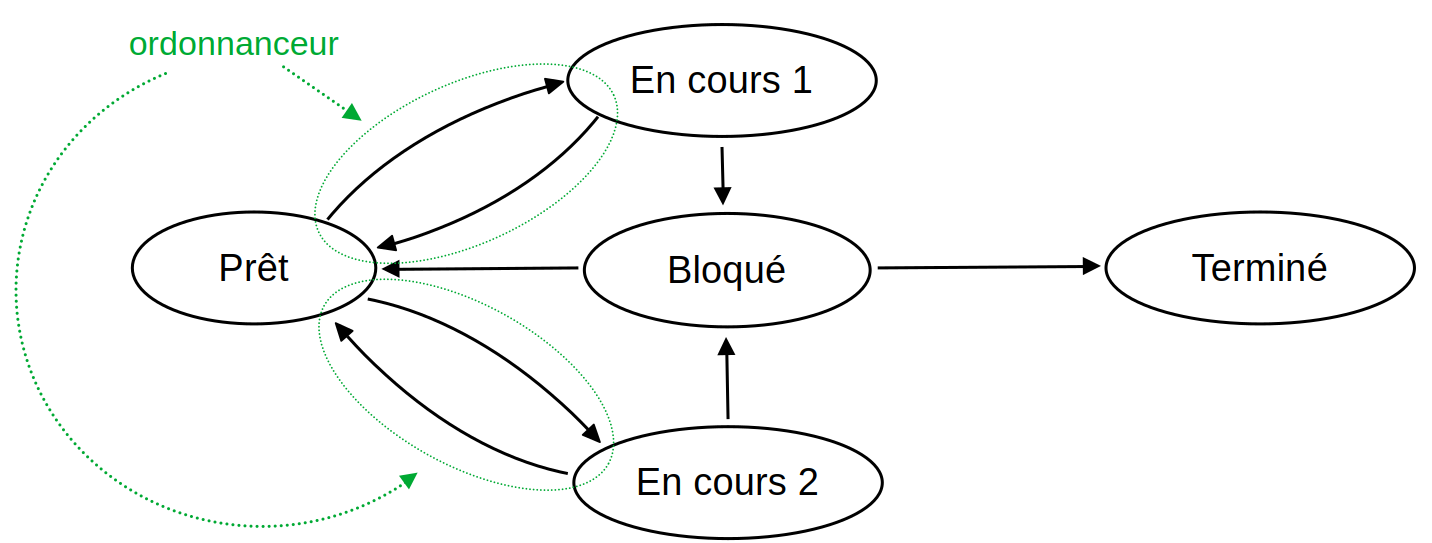
\includegraphics[width=0.9\linewidth]{lecon/17-ordonnancement/graphe_etat.png}\\
	Cycle de vie d'un processus
\end{center}

\begin{com}
	A faire. Mais à comparer avec le truc de Malory, parfois mieux que notre truc à nous.
\end{com}

\chapter{Gestion et coordination de multiples fils d'exécution} \label{L18}
\dev{Emile Martinez}{}

\section{Gestion par la machine (Terminale)}

\subsection{Motivation}

Lorsque vous utilisez votre PC, vous éxécutez des dizaines de programmes «en même temps» (lecture de courriel, taper au clavier, écouter de la musique...). Pourtant, votre PC a un nombre limité de processeurs. Comment fonctionne cette illusion ?

\subsection{Exécution concurrente}

\begin{definition}
	Un processus est un programme en cours d'exécution sur un ordinateur. Il dispose d'une zone mémoire en RAM. Le système d'exécution identifie les processus grâce à un numéro unique appelé PID.
\end{definition}

\begin{definition}[Exécution concurrente]
	Deux processus s'exécutent en concurrence si les intervalles entre leur commencement et leur fin respective sont non disjoints.
\end{definition}

\begin{principe}[Fonctionnement de l'exécution concurrente]
	Le système d'exploitation peut interrompre un processus en cours pour exécuter du code qui lui est propre. Il peut alors, à intervalles réguliers, décider à quelle tâche en cours il rend la main. 
	
	Le rôle de l'ordonnanceur est de choisir le prochain processus à exécuter parmi une liste de processus candidats. 
\end{principe}

\begin{center}
	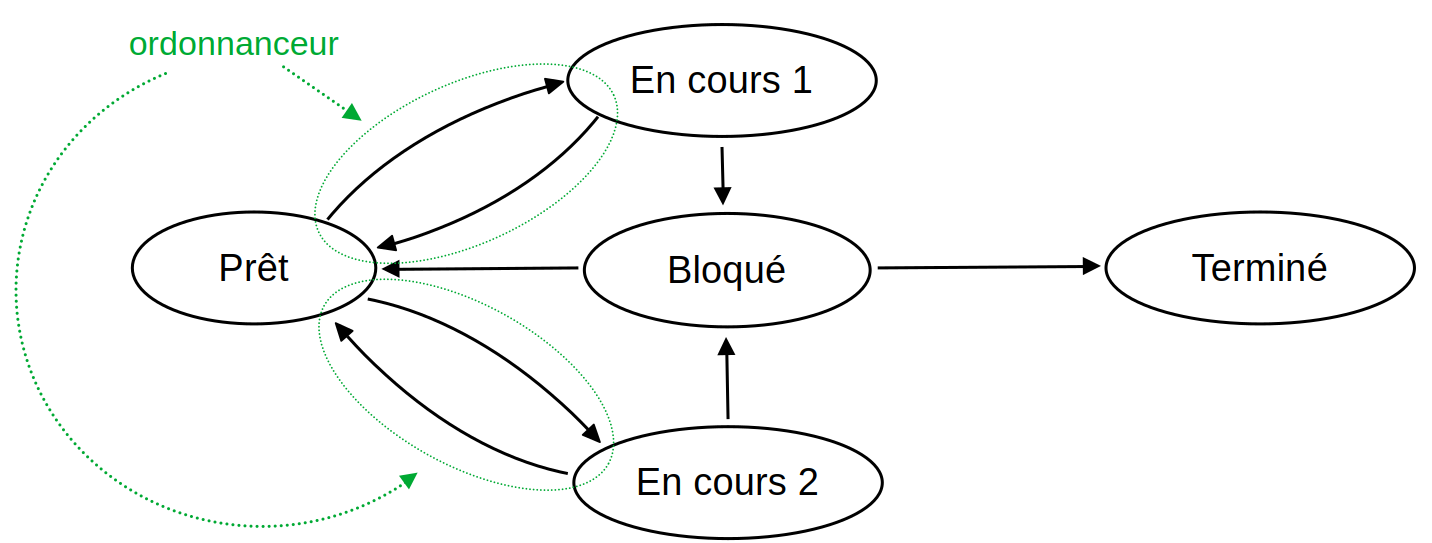
\includegraphics[width=0.9\linewidth]{lecon/17-ordonnancement/graphe_etat.png}\\
	Cycle de vie d'un processus
\end{center}

\subsection{L'ordonnanceur}

On peut vouloir des garanties sur la manière dont l'ordonnanceur choisit ses tâches.

\begin{definition}
	On dit qu'il y a absence de famines (ou vivacité) si aucun processus n'attend indéfiniment.
\end{definition}

\begin{definition}
	On dit qu'il y a équité si aucun processus n'est favorisé.
\end{definition}

\begin{algo}[Algorithme du tourniquet]
	L'ordonnanceur définit un intervalle de temps $\tau$. 
	
	Il place les processus en attente dans une file selon leur ordre d'arrivée (PAPS).
	
	Tant que la file est non vide, il en sort le premier et l’exécute durant tau. Si besoin, il le ré-insert en queue de file.
\end{algo}

\begin{example} Exemple d'exécution sur 3 processus et un seul processeur\\
	\begin{center}
		
		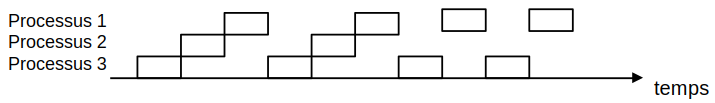
\includegraphics[width=0.8\linewidth]{lecon/18-fil/tourniquet.png}
	\end{center}
\end{example}

\begin{proposition}
	L'algorithme du tourniquet garantie l'équité et l'absence de famine.
\end{proposition}

\begin{rem}
	Certains processus étant plus importants que d'autres, on peut adapter le temps tau à chaque processus, en fonction de leur priorité.
\end{rem}

\subsection{Commande unix de gestion de processus}

\noindent \begin{minipage}{0.3\linewidth}
	\begin{lstlisting}
$ ps
	\end{lstlisting}
\end{minipage}\quad\begin{minipage}{0.6\linewidth}
	permet d'afficher les processus en cours, et leur taux d'occupation du processeur et de la mémoire. 
\end{minipage}\\

\noindent \begin{minipage}{0.3\linewidth}
	\begin{lstlisting}
$kill 6555
	\end{lstlisting}
\end{minipage}\quad\begin{minipage}{0.6\linewidth}
	envoie un  signal de terminaison au processus de PID 6555. (Pour une application graphique, c'est ce que fait la croix rouge)
\end{minipage}\\

\noindent \begin{minipage}{0.3\linewidth}
	\begin{lstlisting}
$top
	\end{lstlisting}
\end{minipage}\quad\begin{minipage}{0.6\linewidth}
	affiche la liste des processus prêts et en cours.
\end{minipage}

\section{Gestion par l'utilisateur (prépa)}

\subsection{Motivation}

\begin{definition}
	Un fil d'exécution (thread en anglais) est un sous processus qui partage la mémoire avec les autres fils du processus.
\end{definition}

\begin{impl}
	En C, un programme peut lancer d'autres fils d'exécution, de type \texttt{pthread\_t} et que l'on lance avec la fonction \texttt{pthread\_create}
\end{impl}

\begin{idee}
	On peut alors gérer des choses en parallèle
\end{idee}

\begin{example}
	\label{18-somme-para} \normalfont
	Somme parallélisée d'un tableau T de taille 2m.\\\\
	\begin{minipage}{0.45\linewidth}
		Fil 1 :
		\begin{lstlisting}[style=CStyle]
for(int i = 0; i < m; i++){
	int s = res + T[2*i];
	res = s;  }\end{lstlisting}
	\end{minipage} \quad
	\begin{minipage}{0.45\linewidth}
		Fil 2:
	\begin{lstlisting}[style=CStyle]
for(int i = 0; i < m; i++){
	int s = res + T[2*i + 1];
	res = s;  }\end{lstlisting}
	\end{minipage}\\
	On peut donc aller deux fois plus vite.
	
	\paragraph{Question :} Que se passe-t-il sur l'exécution F1:1 $\to$ F2:2 $\to$ F1:3 $\to$ F2:3 ?
\end{example}

\subsection{Les verrous}

\begin{definition}
	Le problème de l'exclusion mutuelle consiste à garantir que deux fils d'exécution n'essaieront pas d'exécuter simultanément un morceau de code prédéfini.
\end{definition}

\begin{example}
	Les lignes 2 et 3 pour les fils 1 et 2 de l'exemple \ref{18-somme-para}.
\end{example}

\begin{definition}
	Un verrou (ou mutex) est une structure de données permettant deux opérations : \begin{itemize}
		\item \texttt{prendre()} : appel bloquant qui demande l'accès au verrou
		\item \texttt{rendre()} : appel qui libère le verrou
	\end{itemize}
\end{definition}

\begin{proposition}
	Une implémentation efficace des verrous devrait garantir l'exclusion mutuelle, l'absence de famine et l'équité.
\end{proposition}

\begin{algo}
	L'algorithme de Peterson propose une implémentation des verrous pour deux fils vérifiant ces propriétés.
\end{algo}

\paragraph{Développement :} Présentation de l'algorithme de Peterson et preuve de fonctionnement.

Extension à n fils d'exécution :
\begin{algo} \normalfont Algorithme de la boulangerie de Lamport\\
\begin{minipage}{0.6\linewidth}
	\begin{lstlisting}[style=CStyle]   
void prendre(int i ){
	Acq[i] = 1;
	int t = 0;
	for(int j = 0; j < n; j++)
		t = MAX(t, num[j]);
	num[i] = t + 1;
	Acq[i] = 0;
	
	for(int j = 0; j < n; j++){
		while (acq[j] == 1);
		while (num[j] == 1 && (num[j] < num[i] 
			|| (num[j] == num[i] && j < i)) );
	}
}

void rendre(int i){
	num[i] = 0;
}\end{lstlisting}
\end{minipage}
\begin{minipage}{0.25\linewidth}
	$\begin{array}{l}
	\left. \begin{array}{c} \\ \\ \\ \\ \\ \end{array} \right\} \begin{array}{c} \\ \\ \text{Obtenir un} \\\text{numéro} \\ \\ \end{array} \\
	\\
	\left. \begin{array}{c} \\ \\ \\ \\ \end{array} \right\} \begin{array}{c} \\ \text{Attendre son} \\\text{tour pour prendre} \\ \text{le verrou} \\ \end{array}
	\\ \\ \\ \\ \\
	\end{array}
	$
\end{minipage}
\end{algo}

\paragraph{Analogie :} On prend un ticket dans une boulangerie, et on attend que ce soit notre tour.

\begin{rem}
	L'attente ici est active (on effectue des opérations quand on attend)
\end{rem}

\begin{impl}
	\normalfont
	En C : Les verrous sont disponibles dans la bibliothèque pthread. \begin{itemize}[label=]
		\item type : \texttt{pthread\_mutex\_t}
		\item initialisation : \texttt{pthread\_mutex\_init(pthread\_mutex\_t *m, NULL)}
		\item prendre : \texttt{pthread\_mutex\_lock(pthread\_mutex\_t *m)}
		\item rendre : \texttt{pthread\_mutex\_unlock(pthread\_mutex\_t *m)}
	\end{itemize}
\end{impl}

\begin{rem}
	Une mauvaise utilisation des verrous peut créer des interblocages.
\end{rem}

\begin{example} \enspace\\ \normalfont
	\begin{minipage}{0.3\linewidth}
	Fil 1 :
	\begin{lstlisting}[style=CStyle]
prendre(m1);
prendre(m2);\end{lstlisting}
\end{minipage} \quad
\begin{minipage}{0.3\linewidth}
	Fil 2:
	\begin{lstlisting}[style=CStyle]
prendre(m2);
prendre(m1);\end{lstlisting}
\end{minipage}
\end{example}

\begin{com}
	Ici on ne prend pas un exemple plus gros, comme le dîner des philosophes, car ici on ne veut pas s'étendre sur ça, simplement faire une ouverture, et mentionner le problème.
\end{com}

\section{Les sémaphores}

\paragraph{Analogie :} Tableau des clés d'un hôtel

\begin{definition}
	Un sémaphore est un compteur qui propose les opérations suivantes :
	\begin{itemize}
		\item Initialiser à une valeur entière
		\item décrémenter : appel bloquant, décrémente le compteur s'il est positif, attend qu'il le soit sinon
		\item incrémenter : incrémente le compteur. S'il devient positif, cela libère un fil si un attendait
	\end{itemize} 
\end{definition}

\begin{appl}
	Limiter l'accès à une ressource à $n$ fils.
\end{appl}

\begin{com}
	On ne s’appesantit pas sur cette application au vu de sa complexité. Donc même si c'est l'application la plus directe et que dans un vrai cours, on aurait peut-être ici un petit programme l'utilisant pour illustrer le concept, on se concentre nous sur des choses plus importantes.
\end{com}

\begin{rem}
	On peut implémenter un verrou par un sémaphore initialisé à 1.
\end{rem}

\begin{impl}
	Les sémaphores sont disponibles dans la bibliothèque semaphore.h.
	\begin{itemize}
		\item type : \texttt{sem\_t}
		\item initialisation : \texttt{sem\_init}
		\item décrémenter : \texttt{sem\_wait}
		\item incrémenter : \texttt{sem\_post}
	\end{itemize}
\end{impl}

\begin{proposition}
	L'implémentation des sémaphore est faites (normalement) sans attente active.
\end{proposition}

\begin{appl}[Problème du rendez-vous]
	On a p fils qui doivent se synchroniser. Chacun travaillant en deux phases. Dans la première phase, tous les fils sont indépendants et peuvent s’exécuter simultanément. La deuxième phase d'un fil ne peut débuter que si tous les fils ont terminé la première.\\
	
	On peut résoudre ce problème à l'aide de sémaphore.
\end{appl}

\paragraph{Développement :} Solutions aux problèmes du rendez-vous

\begin{appl}[Producteur / Consommateur] \normalfont
	On dispose d'un tampon de taille N, et on a deux types de fils : \begin{itemize}
		\item des producteurs qui produisent des ressources et les stockent dans le tampon
		\item des consommateurs qui consomment les données produites (consommer une donnée libère son emplacement)
	\end{itemize}
	
	Pour que la donnée consommée soit la plus vieille, le tampon est circulaire :
	\begin{center}
		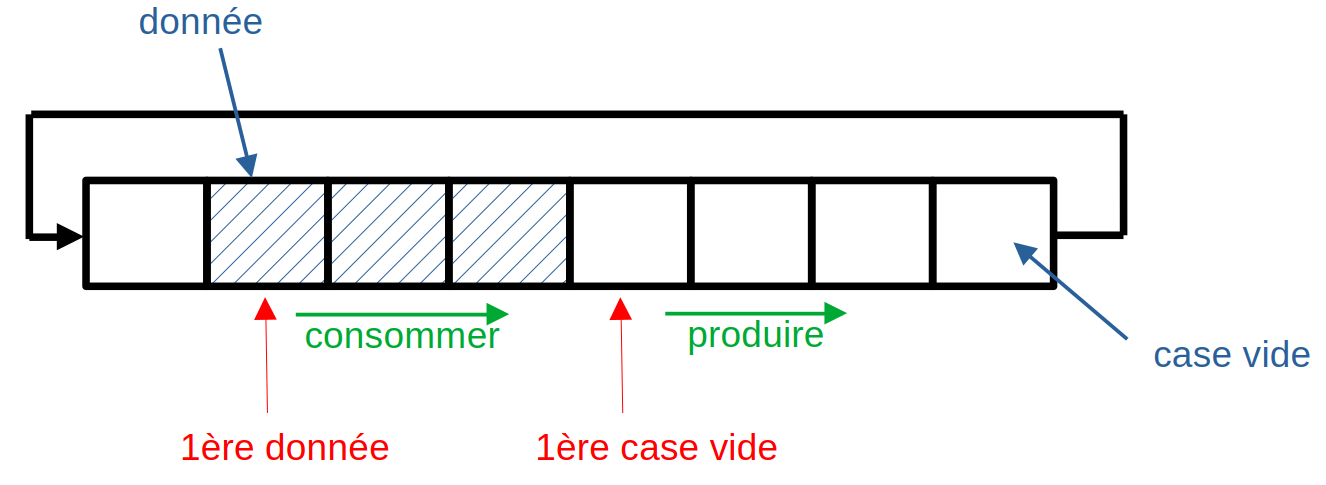
\includegraphics[width=0.7\linewidth]{lecon/18-fil/prod-cons.png}
	\end{center}
	
	\paragraph{Problème :} \begin{itemize}
		\item l'accès au tampon est partagé
		\item les consommateurs doivent attendre qu'une place soir produite
		\item les producteurs doivent attendre que de la place soit libérée dans le tampon.
	\end{itemize}
	
	\paragraph{Solution :} On utilise un sémaphore indiquant le nombre données disponibles et un le nombre de cases disponibles.
	
	\begin{lstlisting}[style=CStyle]
sem_t mutex, vide, plein;
sem_init(&mutex, 0, 1);
sem_init(&vide, 0, N);
sem_init(&plein, 0, 0);\end{lstlisting}

\begin{minipage}{0.45\textwidth}
		Producteur :
		\begin{lstlisting}[style=Cstyle]
int item;
while(1){
	item = produire_item()
	// On attend un place
	sem_wait(&vide);
	sem_wait(&mutex);
	insert_item(item);
	sem_post(&mutex);
	// On la remplie
	sem_post(&plein);
}\end{lstlisting}
	\end{minipage}\qquad
	\begin{minipage}{0.45\textwidth}
		Consommateur :
		\begin{lstlisting}[style=Cstyle]
int item;
while(1){
	// On attend un element
	sem_wait(&plein);
	sem_wait(&mutex);
	item = remove_item();
	sem_post(&mutex);
	// On libere une place
	sem_post(&vide);
	consomer_item(item);
}\end{lstlisting}
	\end{minipage}
	
\end{appl}

\begin{com}
	Par manque de place, on peut moins s'étendre et ne pas écrire l'algorithme, se contenter de dire qu'on a un sémaphore qui compte les places vides et un les places pleines. (et éventuellement virer le dessin)
\end{com}

\begin{rem}
	On peut implémenter un sémaphore par de l'attente active et des verrous. Donc naturellement, ce qu'apporte souvent les sémaphores, par rapport au verrou, c'est moins d'attente active.
\end{rem}

\begin{com}
	Cette remarque, car si on a des élèves un peu rapide, il pourrait trouver assez facilement des solutions n'utilisant que des verrous, et donc se poserait la question de la pertinence des sémaphores dans ce contexte. L'intérêt des sémaphores vient alors de la suppression de l'attente active.
\end{com}

\begin{com}
	On ne mentionne pas tous les problèmes possibles liés aux sémpahores, car ici dans cette leçon on doit parler de plein d'aspects différents. On se limite alors à en expliquer le fonctionnement global et à les illustrer.
\end{com}

\chapter{Mémoire : du bit à l’abstraction vue par les processus.} \label{L19}

\chapter{Problèmes et stratégies de cohérence et de synchronisation.} \label{L20}
\dev{Emile Martinez}{}

\section{Introduction}

\begin{definition}
	Un processus est un programme en cours d'exécution sur un ordinateur. Il dispose d'une zone mémoire en RAM (pour stocker la pile, les données de travail, etc.). Le système d'exécution identifie les processus grâce à un numéro unique appelé PID. 
\end{definition}

\begin{definition}
	Un fil d'exécution (ou thread) est un sous processus qui partage la mémoire avec les autres threads du processus.
\end{definition}

\begin{impl}
	En C, un programme peut lancer d'autres fils d'exécution, de type \texttt{pthread\_t} et que l'on lance avec la fonction \texttt{pthread\_create}
\end{impl}

\begin{example}
	\label{20-somme-para} \normalfont
	Somme parallélisée d'un tableau T de taille 2m.\\\\
	\begin{minipage}{0.45\linewidth}
		Fil 1 :
		\begin{lstlisting}[style=CStyle]
			for(int i = 0; i < m; i++){
				int s = res + T[2*i];
				res = s;  }\end{lstlisting}
	\end{minipage} \quad
	\begin{minipage}{0.45\linewidth}
		Fil 2:
		\begin{lstlisting}[style=CStyle]
			for(int i = 0; i < m; i++){
				int s = res + T[2*i + 1];
				res = s;  }\end{lstlisting}
	\end{minipage}\\
	On peut donc aller deux fois plus vite.
	
	\paragraph{Question :} Que se passe-t-il sur l'exécution F1:1 $\to$ F2:2 $\to$ F1:3 $\to$ F2:3 ?
\end{example}

\subsection{Définitions générales}

\begin{definition}
	On appelle appel bloquant un appel à une fonction qui attendra que les conditions soit réunies avant de terminer.
\end{definition}

\begin{example}
	L'appel à \texttt{recv} en C qui attend que quelque chose arrive pour terminer.
\end{example}

\begin{definition}
	On dit qu'il y a absence de famine (ou vivacité) si aucun fil n'attend indéfiniment.
\end{definition}

\begin{definition}
	On dit qu'il y a équité si aucun processus n'est favorisé.
\end{definition}

\section{Exclusion mutuelle et verrous}

\subsection{Définition}

\begin{definition}
	Une section critique est un ensemble de morceau de code qui ne doit être exécute que par un seul fil à la fois.
	
	Le problème de l'exclusion mutuelle est le problème consistant à garantir qu'on aura toujours au plus un fil dans une section critique.
\end{definition}

\begin{example}
	Les lignes 2 et 3 pour les fils 1 et 2 de l'exemple \ref{20-somme-para}.
\end{example}

\begin{rem}
	Dans une section critique, les morceaux de code ne sont pas forcément les mêmes pour chaque fil (si un fil ne fais que lire quand l'autre ne fais qu'écrire dans une case partagée, leurs codes incompatibles n'est pas le même).
\end{rem}

\paragraph{Solution :} Les verrous

\begin{definition}
	Un verrou (ou mutex) est une structure de données permettant deux opérations : \begin{itemize}
		\item \texttt{prendre()} : appel bloquant qui demande l'accès au verrou
		\item \texttt{rendre()} : appel qui libère le verrou
	\end{itemize}
\end{definition}

\begin{proposition}
	Une implémentation efficace des verrous devrait garantir l'exclusion mutuelle, l'absence de famine et l'équité.
\end{proposition}

\subsection{Implémentation des verrous pour 2 fils}

\begin{definition}
	Une opération est dite atomique si elle ne peut pas être interrompue. Dans notre cas, une opération atomique correspond à une instruction en langage machine. On a notamment les opérations : \begin{itemize}
		\item lire une case mémoire
		\item écrire une case mémoire
		\item effectuer une opération arithmétique/logique
	\end{itemize}
\end{definition}

\begin{rem}
	Attention ! Une opération dans un langage de programmation n'est pas atomique en général.
\end{rem}

\begin{proposition}
	Si deux fils écrivent la même case mémoire simultanément, la case mémoire contiendra soit la valeur du premier fils soit celle du second. De même, si un fil lis dans une case quand un autre écrit, la valeur sera écrite et le premier fil lira la valeur précédente ou la valeur actualisée.
\end{proposition}

\begin{algo}
	Algorithme de Peterson pour un verrou à deux fils \normalfont
	\begin{lstlisting}
tour = -1
veut_entrer = [false, false]

rendre(i): 
	veut_entrer[i] = true
	tour = 1-i

	while(tour == 1-i && veut_entrer[1-i]) {}

prendre(i): 
	veut_entrer[i] = false
	\end{lstlisting}
\end{algo}

\paragraph{Développement :} Présentation de l'algorithme de Peterson.

\subsection{Généralisation à n fils}

\begin{algo} \normalfont Algorithme de la boulangerie de Lamport\\
	\begin{minipage}{0.6\linewidth}
		\begin{lstlisting}[style=CStyle]   
void prendre(int i ){
	Acq[i] = 1;
	int t = 0;
	for(int j = 0; j < n; j++)
	t = MAX(t, num[j]);
	num[i] = t + 1;
	Acq[i] = 0;
	
	for(int j = 0; j < n; j++){
		while (acq[j] == 1);
		while (num[j] == 1 && (num[j] < num[i] 
		|| (num[j] == num[i] && j < i)) );
	}
}

void rendre(int i){
	num[i] = 0;
}\end{lstlisting}
	\end{minipage}
	\begin{minipage}{0.25\linewidth}
		$\begin{array}{l}
			\left. \begin{array}{c} \\ \\ \\ \\ \\ \end{array} \right\} \begin{array}{c} \\ \\ \text{Obtenir un} \\\text{numéro} \\ \\ \end{array} \\
			\\
			\left. \begin{array}{c} \\ \\ \\ \\ \end{array} \right\} \begin{array}{c} \\ \text{Attendre son} \\\text{tour pour prendre} \\ \text{le verrou} \\ \end{array}
			\\ \\ \\ \\ \\
		\end{array}
		$
	\end{minipage}
\end{algo}

\paragraph{Analogie :} On prend un ticket dans une boulangerie, et on attend que ce soit notre tour.

\begin{rem}
	Dans nos implémentations, l'attente est active.
\end{rem}

\begin{impl}
	\normalfont
	En C : Les verrous sont disponibles dans la bibliothèque pthread. \begin{itemize}[label=]
		\item type : \texttt{pthread\_mutex\_t}
		\item initialisation : \texttt{pthread\_mutex\_init(pthread\_mutex\_t *m, NULL)}
		\item prendre : \texttt{pthread\_mutex\_lock(pthread\_mutex\_t *m)}
		\item rendre : \texttt{pthread\_mutex\_unlock(pthread\_mutex\_t *m)}
	\end{itemize}
\end{impl}

\section{Synchronisation et sémaphores}

\begin{impl}
	Pour synchroniser des fils, la commande \texttt{pthread\_join} de la bibliothèque pthread permet à un fil d'attendre la fin et de récupérer la valeur de retour d'un ou de n'importe lequel de ces fil fils.
\end{impl}

\begin{rem}
    Néanmoins, on peut souhaiter plus de synchronisation entre les fils.
\end{rem}

\subsection{Sémaphore et synchronisation}
\textit{Bon on a un peu de redondances sur les titres là}

\paragraph{Analogie :} Tableau des clés d'un hôtel

\begin{definition}
	Un sémaphore est un compteur qui propose les opérations suivantes :
	\begin{itemize}
		\item Initialiser à une valeur entière
		\item décrémenter : appel bloquant, décrémente le compteur s'il est positif, attend qu'il le soit sinon
		\item incrémenter : incrémente le compteur. S'il devient positif, cela libère un fil si un attendait
	\end{itemize} 
\end{definition}

\begin{appl}
	Limiter l'accès à une ressource à $n$ fils.
\end{appl}

\begin{com}
	On ne s’appesantit pas sur cette application au vu de sa complexité. Donc même si c'est l'application la plus directe et que dans un vrai cours, on aurait peut-être ici un petit programme l'utilisant pour illustrer le concept, on se concentre nous sur des choses plus importantes.
\end{com}

\begin{rem}
	On peut implémenter un verrou par un sémaphore initialisé à 1.
\end{rem}

\begin{impl}
	Les sémaphores sont disponibles dans la bibliothèque semaphore.h.
	\begin{itemize}
		\item type : \texttt{sem\_t}
		\item initialisation : \texttt{sem\_init}
		\item décrémenter : \texttt{sem\_wait}
		\item incrémenter : \texttt{sem\_post}
	\end{itemize}
\end{impl}

\begin{proposition}
	L'implémentation des sémaphore est faites (normalement) sans attente active.
\end{proposition}

\begin{appl}[Problème du rendez-vous]
	On a p fils qui doivent se synchroniser. Chacun travaillant en deux phases. Dans la première phase, tous les fils sont indépendants et peuvent s’exécuter simultanément. La deuxième phase d'un fil ne peut débuter que si tous les fils ont terminé la première.\\
	
	On peut résoudre ce problème à l'aide de sémaphore.
\end{appl}

\paragraph{Développement :} Solutions aux problèmes du rendez-vous

\subsection{Cas classique d'utilisation}

\begin{appl}[Problème du rendez-vous]
	On a p fils qui doivent se synchroniser. Chacun travaillant en deux phases. Dans la première phase, tous les fils sont indépendants et peuvent s’exécuter simultanément. La deuxième phase d'un fil ne peut débuter que si tous les fils ont terminé la première.\\
	
	On peut résoudre ce problème à l'aide de sémaphore.
\end{appl}

\paragraph{Développement :} Solutions aux problèmes du rendez-vous

\begin{appl}[Producteur / Consommateur] \normalfont
	On dispose d'un tampon de taille N, et on a deux types de fils : \begin{itemize}
		\item des producteurs qui produisent des ressources et les stockent dans le tampon
		\item des consommateurs qui consomment les données produites (consommer une donnée libère son emplacement)
	\end{itemize}
	
	Pour que la donnée consommée soit la plus vieille, le tampon est circulaire :
	\begin{center}
		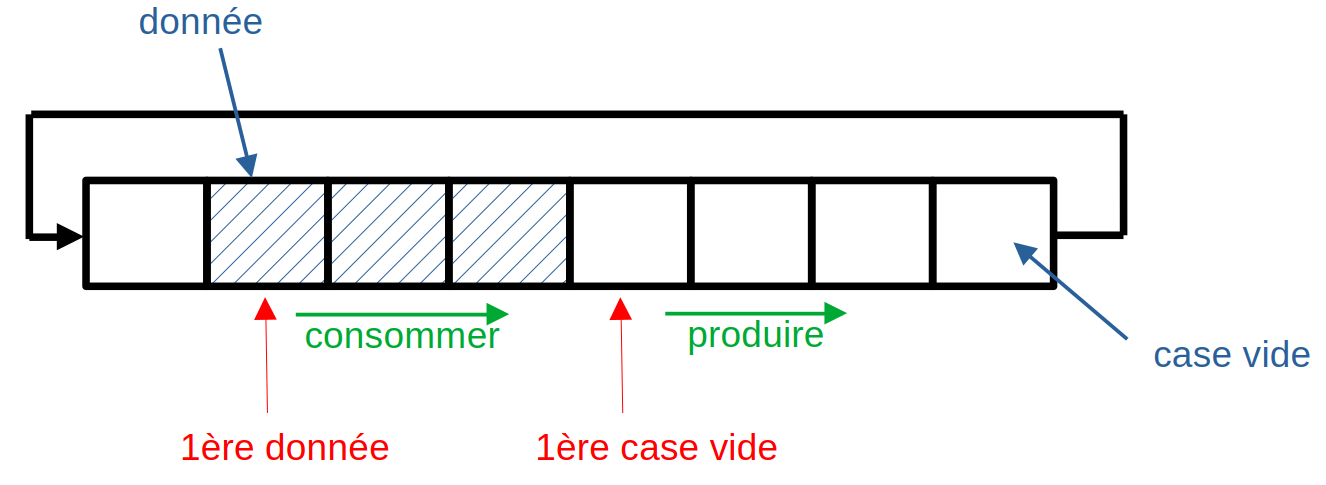
\includegraphics[width=0.7\linewidth]{lecon/18-fil/prod-cons.png}
	\end{center}
	
	\paragraph{Problème :} \begin{itemize}
		\item l'accès au tampon est partagé
		\item les consommateurs doivent attendre qu'une place soir produite
		\item les producteurs doivent attendre que de la place soit libérée dans le tampon.
	\end{itemize}
	
	\paragraph{Solution :} On utilise un sémaphore indiquant le nombre données disponibles et un le nombre de cases disponibles.
	
	\begin{lstlisting}[style=CStyle]
		sem_t mutex, vide, plein;
		sem_init(&mutex, 0, 1);
		sem_init(&vide, 0, N);
		sem_init(&plein, 0, 0);\end{lstlisting}
	
	\begin{minipage}{0.45\textwidth}
		Producteur :
		\begin{lstlisting}[style=Cstyle]
			int item;
			while(1){
				item = produire_item()
				// On attend un place
				sem_wait(&vide);
				sem_wait(&mutex);
				insert_item(item);
				sem_post(&mutex);
				// On la remplie
				sem_post(&plein);
		}\end{lstlisting}
	\end{minipage}\qquad
	\begin{minipage}{0.45\textwidth}
		Consommateur :
		\begin{lstlisting}[style=Cstyle]
			int item;
			while(1){
				// On attend un element
				sem_wait(&plein);
				sem_wait(&mutex);
				item = remove_item();
				sem_post(&mutex);
				// On libere une place
				sem_post(&vide);
				consomer_item(item);
		}\end{lstlisting}
	\end{minipage}
	
\end{appl}

\begin{com}
	Par manque de place, on peut moins s'étendre et ne pas écrire l'algorithme, se contenter de dire qu'on a un sémaphore qui compte les places vides et un les places pleines. (et éventuellement virer le dessin)
\end{com}

\begin{rem}
	On peut implémenter un sémaphore par de l'attente active et des verrous. Donc naturellement, ce qu'apporte souvent les sémaphores, par rapport au verrou, c'est moins d'attente active.
\end{rem}

\begin{com}
	Cette remarque, car si on a des élèves un peu rapide, il pourrait trouver assez facilement des solutions n'utilisant que des verrous, et donc se poserait la question de la pertinence des sémaphores dans ce contexte. L'intérêt des sémaphores vient alors de la suppression de l'attente active.
\end{com}

\section{Interblocage}

\begin{definition}
	On dit qu'il y a interblocage quand tous les fils sont bloqués et ne seront jamais libérés.
\end{definition}

\begin{example} \enspace\\ \normalfont
	\begin{minipage}{0.3\linewidth}
		Fil 1 :
		\begin{lstlisting}[style=CStyle]
			prendre(m1);
			prendre(m2);\end{lstlisting}
	\end{minipage} \quad
	\begin{minipage}{0.3\linewidth}
		Fil 2:
		\begin{lstlisting}[style=CStyle]
			prendre(m2);
			prendre(m1);\end{lstlisting}
	\end{minipage}
\end{example}

\begin{definition}[Diner des philosophes]
	On a cinq philosophes autour d'une table ronde et une fourchette entre chaque. Chaque philosophe alterne moment de faim et de réflexion. Quand il a faim, il attend de prendre ses deux fourchettes, puis il mange, les repose etc.
\end{definition}

\paragraph{Solution naïve :} Un verrou par fourchette, chaque philosopge attend de prendre sa fourchette gauche, puis sa droite

\paragraph{Problème :} Interblocage

\begin{exercise}
	L'implémenter pour observer cet interblocage
\end{exercise}

\paragraph{Solution :} \begin{itemize}
	\item Avec des verrous : chaque philosophe essaye d'abord de prendre sa fourchette de plus petit indice
	\item Avec des sémaphores : On n'autorise que 4 philosophes à essayer de prendre des fourchettes grâce à un sémaphore
\end{itemize}

\begin{com}
	Bon on pourrait aussi mettre dans cette partie un petit dessin.
\end{com}

\chapter{Stockage et manipulation de données, des fichiers aux bases de données.} \label{L21}
\dev{Emile Martinez}{Balabonski, Barra}

La mémoire d'un programme meurt avec lui. Néanmoins, on souhaite garder des données plus perennement.

La mémoire d'un ordinateur est alors une série de milliards de bits, parmi lesquels coexistent tout et n'importe quoi. On veut les organiser de façon à rendre leur accès le plus simple et rapide possible.

\section{Fichiers}

\subsection{Organisation et manipulation}

\begin{definition}
	Un fichier est un ensemble de données. C'est l'unité de stockage manipulé par l'utilisateur.
\end{definition}

\begin{definition}
	Pour organiser des données de manière persistante sur un disque on utilise une arborescence de fichier. La norme POSIX, suivie par la plupart des OS (linux, Mac, android) définit cette organisation et sa manipulation.
\end{definition}

\begin{example}
	Arborescence de fichier linux (obtenue par la commande \texttt{tree})\\
	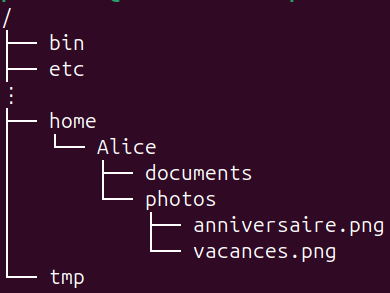
\includegraphics[width=0.4\linewidth]{lecon/21-fichier/arborescence.png}
\end{example}

\begin{definition}
	Le chemin d'accès vers un fichier est soit exprimé de manière absolu (depuis la racine) soit depuis le répertoire courant
\end{definition}

\begin{impl}
	On peut accèder et manipuler l'arborescence de fichier depuis un invite de commande (shell ou terminal) avec les commandes suivantes : \begin{itemize}[label=$\bullet$]
	\item pwd : affiche le repertoire courant
	\item cd chemin : change le repertoire courant pour la cible du chemin
	\item mkdir/touch : créer un dossier/un fichier
	\item cp/mv/rm : copie/ déplace et renomme / supprime
	\item ls  : liste le contenu d'un repertoire
	\end{itemize}
\end{impl}

\begin{exercise}
	Prise en main des commandes du shell avec appuie sur l'utilisation du man.
\end{exercise}

\begin{impl}
	La commande ls -l permet de faire apparaitre des informations supplémentaires sur les fichiers : propriétaire, groupe prioritaire, taille, dernière modification et autorisations :
	\normalfont
	$$ \underset{\circled{1}}{\underbrace{\texttt{\enspace\enspace-}}} \underset{\circled{2}}{\underbrace{\texttt{rwx}}}\underset{\circled{3}}{\underbrace{\texttt{r--}}}\underset{\circled{4}}{\underbrace{\texttt{r--}}}$$
	
	$\circled{1}$ : type de fichier : \begin{itemize}
		\item[] \qquad \texttt{d} : répertoire
		\item[] \qquad \texttt{l} : lien symbolique
		\item[] \qquad \texttt{-} : autre
	\end{itemize}
	
	$\circled{2}\circled{3}\circled{4}$ : \begin{itemize}
		\item[] \qquad \texttt{r} : read
		\item[] \qquad \texttt{w} : write
		\item[] \qquad \texttt{x} : execute
	\end{itemize}
	
	$\circled{2}$ : permissions propriétaire
	
	$\circled{3}$ : permissions groupe
	
	$\circled{4}$ : permissions tous
	
	
\end{impl}

\begin{rem}
	Pour Linux, "tout est un fichier" : les codes sources, les exécutables, mais aussi les périphériques qui peuvent être lus (souris, clavier) ou écrits (écran) comme des fichiers
\end{rem}

\begin{proposition}
	Plusieurs systèmes de fichiers (volume dans la mémoire) peuvent cohabiter sur un même ordinateur, avec chacun leur racine
\end{proposition}

\begin{example}
	Les C::, D::, E::, etc. sous Windows sont autant de système de fichiers
\end{example}

\begin{rem}
	Sous Linux, tous les espaces de stockages montés partagent la même arborescence
\end{rem}

\subsection{Stockage}

Il existe plusieurs manières de faire un système de fichier (FAT32, ext4, \dots) définissant des primitives de gestion des fichiers ainsi que des structures de données pour la gestion des espaces libres.

\begin{definition}
	On découpe alors les fichiers en blocs de quelques ko. Le système de fichier ne manipulera alors que des blocs.
\end{definition}

\begin{definition}
	Un fichier étant souvent trop grand pour un unique bloc, il est séparé en plusieurs blocs : \begin{itemize}
	
	\item allocation contigüe : les blocs sont contigües sur le disque \\
	$\to$ accès séquentiel rapide mais fragmentation et difficulté à créer ou etendre des fichiers.
	
	\item allocation chaînée : les blocs peuvent être n'importe où, chaque bloc contenant l'adresse du suivant\\
	$\to$ bonne utilisation de la mémoire, création extension facile mais accès séquentiel lent
	
	On dispose alors parfois d'une table d'allocation de fichiers
	
	\item l’allocation indexée : les adresses des blocs constituant un même fichier sont rangées dans une table, appelée index, elle-même con
	
	tenue dans un ou plusieurs blocs.
	
	$\to$ bonne accès séquentiel et extension facile, mais taille de fichier maximales et utilisation de mémoire annexe (visible surtout sur les petits fichiers)
	\end{itemize}
\end{definition}


\begin{definition}
	Chaque fichier se voit associé un numéro inode à un emplacement de stockage. L'inode permet de retrouver dans une table du périphérique de stockage des infos données par \texttt{ls -l}.
\end{definition}

\begin{definition}
	Pour économiser de la place, des liens peuventêtre crées entre des fichiers avec :
	
	\qquad \texttt{ln} : lien physique, l'inode est partagé mais la suppression d'un des fichiers n'impacte pas l'autre
	
	\qquad \texttt{ln -s} : lien symbolique, un nouvel inode est utilisé et le fichier ne contient que le chemin vers sa source.

\end{definition}

\section{Format}

\subsection{Fichier texte}

\begin{definition}
	Un fichier texte représente uniquement une suite de caractères (type char en C ou en OCaml) codé en ASCII.
\end{definition}

\begin{rem}
	C'est le format de fichier de base.
\end{rem}

\begin{rem}
	Il arrive que l'on veuille représenter plus que les 128 caractères qu'autorise l'ASCII (ou 256 pour l'ASCII étendue). On peut alors utiliser des codages sur plus de bits (16 pour l'unicode par exemple).
\end{rem}

\begin{definition}
	Étant le format de fichier le plus basique, il est le plus simple à manipuler. On pourra alors accéder à ces fichiers en langage de programmation :\\
	\begin{tabular}{l|l|l}
		\multicolumn{1}{c}{Fonction} & \multicolumn{1}{|c|}{En C} & \multicolumn{1}{c}{En OCaml}\\
		ouvrir un fichier &  \texttt{fopen(chemin, mode)} & \texttt{open\_in} \\
		fermer un fichier & \texttt{fclose(fichier)} & \texttt{close\_in} \\
		écrire dans un fichier & \texttt{fprintf} & \texttt{input\_line} \\
		lire dans un fichier & \texttt{scanf} & \texttt{output\_line}
	\end{tabular}
\end{definition}

\begin{rem}
	Lorsqu'on utilise \texttt{printf} en C, on écrit dans un fichier particulier : la sortie standard (stdout) qui correspond à l'invite de commande. \texttt{printf} est donc équivalent à \texttt{fprintf(stdout, $\dots$)}. De même, \texttt{scanf} lit dans l'entrée standard (stdin). 
\end{rem}

\begin{definition}
	Pour rediriger la sortie standard, on peut utiliser des commandes : \begin{itemize}
		\item \texttt{commande > filename} : la sortie standard de la commande est écrite ddans le fichier, qui est écrasé.
		\item \texttt{commande >> filemane} : même chose mais sans écraser le fichier. 
		\item \texttt{commande < fichier} : le fichier devient l'entrée standard de la commande
		\item \texttt{commande1 | commande2} : la sortie standard de la première commande est reliée à l'entrée standard de la deuxieme.
	\end{itemize}
\end{definition}

\begin{rem}
	L'écriture étant lente, un tampo est utilisé. On peut forcer l'écriture des tampons avec \texttt{flush} en OCaml et \texttt{fflush} en C.
\end{rem}

\subsection{Formats de fichiers}

Pour représenter plus que des chaînes caractères, on a besoin de définir des formats de fichiers qui indiquent comment interpréter les bits de données. 

\begin{definition}
	Un format de fichier est une convention de représentation de données
\end{definition}

\begin{rem}
	Pour gagner de l'espace, ces formats utilisent souvent des méthodes de compression, avec ou sans perte.
\end{rem}

\begin{example}
	Quelques formats particuliers :
	\begin{itemize}
		\item Le format png stocke et compresse les images sans perte
		\item Le format jpeg stocke des images compressées avec perte
		\item Le formats mp3 stocke des sons compressés avec perte
		\item Le format mp4 combine audio et vidéo
		\item Le format zip compresse sans perte des fichiers quelconques
	\end{itemize}
\end{example}

\begin{rem}
	Le format zip utilise l'algorithme de compression LZW, mais aussi le codage de Huffman.
\end{rem}

\paragraph{Développement :} Présentation de l'algorithme LZW.

\begin{rem}
	Il y a toujours un compromis à faire entre différents objectifs (ex : compression et facilité d'utilisation). Ainsi la plupart des formats se spécialisent dans une utilisation :
	\begin{itemize}
		\item quand on ouvre une image en python, on la transforme en tableau de triplets, quand on la sauvegarde on la recompresse, dans un format moins manipulable
		\item Quand on édite une vidéo, on doit l'exporter à la fin pour passer d'un format manipulable à un format pour la lecture
		\item Quand on compresse des fichiers en .zip, on ne peut plus les modifier ou les lire 
	\end{itemize}raison pour lesquelles on exporte quand on monte une vidéo, pour baser d'un format éditable à un format compressé adapté à la lecture).
\end{rem}

\begin{example}
	Le format CSV (pour comma separated values) est un format de texte brut permettant de stocker des données sous forme de table, permettant ainsi facilement la suppresion, l'ajout, etc.\\
	
	Pour des commandes \{ produit : tomate, prix : 3 quantité : 50, client : Le navet naviguant, adresse : 13 rue du Swag à Tarbes \},  \{ produit : patate, prix : 1, quantité : 30, client : Le navet naviguant, adresse : 13 rue du Swag à Tarbes \},  \dots
	
	Pourrait-on mieux faire ?
\end{example}

\section{Bases de données}

Souvent, les données d'une table ont des redondances, et des liens entre elles (cf exemple au dessus). Pour manipuler des gros volumes de données on ne se contente alors plus alors de fichiers en texte brut.

\begin{definition}
	Le modèle relationnel est une manière de représenter les données en exploitant les relations entre elles.
\end{definition}

\begin{example}
	Un grossistes gérant des commandes.
	\normalfont\\
	\texttt{Produit(\underline{num\_produit}, nom, prix, poids)}\\
	\texttt{Clients(\underline{num\_client}, nom, adresse, ville)}\\
	\texttt{Commande(\underline{\#num\_produit, \#num\_client}, quantite)}\\
	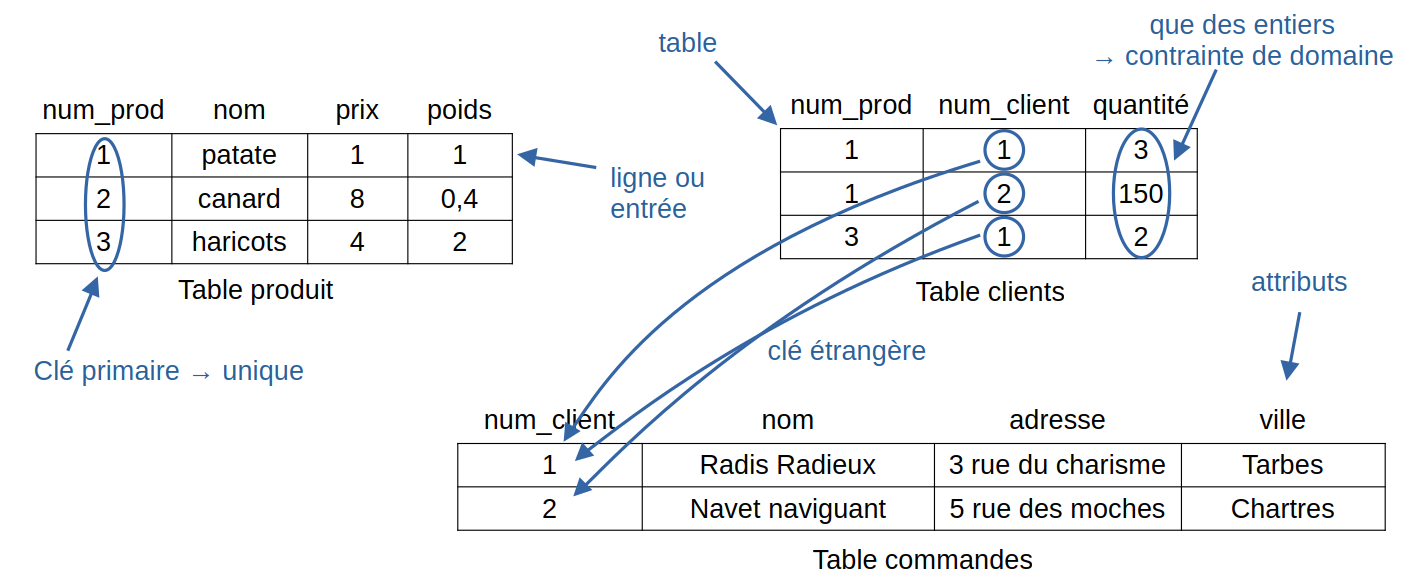
\includegraphics[width=\linewidth]{lecon/21-fichier/schema_bd.png}
\end{example}

\begin{definition}
	Un SGBD (système de gestion de bases de données) est utilisé pour manipuler des données relationnelles, garantissant les propriétés ACID (atomicité, cohérence, isolation et durabilité). On intéragit avec lui à travers le langage SQL.
\end{definition}

\begin{example}
	Le SQL permet de sélectionner certaines données, de les trier, de les filtrer selons certaines conditions, etc \dots
\end{example}

\begin{com}
	Si on a la place ici, on peut insérer des mots clés.
\end{com}

\begin{theorem}[Codd]
	SQL est suffisamment expressif pour quasiment tout ce que l'on souhaite faire
\end{theorem}

\begin{exercise}
	Trouver différentes manières de calculer le max et la division.
\end{exercise}

\paragraph{Développement :} Correction de l'exercice précédent.

\begin{com}
	Ici on pourrait également défendre le fait de faire plutôt l'autre développement de requêtes SQL, introduisant les requêtes, les mots clés de bases, etc. Il s'insère parfaitement dans la leçon, (mieux que ce développement là où il faut justifier que on a introduit aucune syntaxe dans le cours, mais que en vrai ils la connaîtraient), mais c'est un développement moins poussé. Donc on montre moins la puissance de calcul.
\end{com}



\chapter{Fonctions et circuits booléens en architecture des ordinateurs} \label{L22}
\debut{Emile Martinez}{Prépa / Première}{Représentation binaire et pour la première partie : induction, graphe}{}

\section{Cadre théorique (Prépa)}

\subsection{Expression booléenne}

\begin{definition}
	On définit l'ensemble $EB$ des expressions booléennes par induction avec la signature
	\begin{itemize}[label=$\bullet$]
		\item cas de bases : $\top, \,\bot, \,V$ un ensemble de variables
		\item constructeurs :\begin{itemize}[label=$\star$]
			\item $\neg$ un constructeur unaire
			\item $\vee, \, \wedge$ deux constructeurs binaires
		\end{itemize}
	\end{itemize}
\end{definition}

Informellement : $\top, \bot, x \in V$ sont des expressions booléennes, et si $e_1$ et $e_2$ le sont, alors $\neg e_1$, $e_1\vee e_2$, et $e_1 \wedge e_2$ le sont.

\begin{exercise}
	Définir inductivement les variables apparaissant dans une formule et en déduire une définition rigoureuse du nombre de variables d'une fonction.
\end{exercise}

\begin{definition}
	Une valuation est une fonction $\sigma :V \to \{0,1\}$.
	\\
	\\
	On définit alors $[\,]_\sigma$ : $EB \to \{0, 1\}$ par induction sur EB par :\begin{itemize}[label=$\bullet$]
		\item $[\bot]_\sigma = 0$, $[\top]_\sigma = 1$ et $[x]_\sigma = \sigma(x)$ pour $x \in V$
		\item $[e_1 \vee e_2] = \max([e_1]_\sigma, [e_2]\sigma)$
		\item $[e_1 \wedge e_2] = \min([e_1]_\sigma, [e_2]\sigma)$
		\item $[\neg e_1]_\sigma = 1-[e_1]_\sigma$
	\end{itemize}
\end{definition}

\begin{definition}
	Pour $a, b \in EB$, on dit que $a$ et $b$ sont équivalentes noté $a \equiv b$, si $\forall \sigma :V \to \{0,1\}, [a]_\sigma = [b]_\sigma$
\end{definition}

\begin{definition}
	On peut éventuellement définir le XOR (ou exclusif), avec $a\oplus b = (a\vee b)\wedge \neg(a\wedge b) \equiv (a\wedge \neg b)\vee (\neg a\wedge b)$
\end{definition}

\subsection{Fonctions booléennes}

\label{22-1-2}

\begin{definition}
	Une fonction booléenne est une fonction de $\{0, 1\}^n \to \{0, 1\}^m$
\end{definition}

\begin{example}
	$f : \{0,1\}^{64} \to \{0,1\}^{64}$ prenant en entrée le codage (en double) d'un flottant $x$, et renvoyant le codage du flottant de $e^x$
\end{example}

\begin{rem}
	On se limite parfois à $f : \{0,1\}^n \to \{0, 1\}$ (en décomposant $f : \{O, 1\}^n \to \{0, 1\}^m$ en $m$ fonctions sur chaque dimension)
\end{rem}

\begin{definition}[Table de vérité]
	La table de vérité d'une fonction booléenne est la donnée de sa valeur sur toutes ses entrées possibles. On représente la table de vérité de $f:\{0,1\}^n \to \{0,1\}^m$ dans un tableau avec $n+m$ colonnes, et pour chaque éléments de $\{0,1\}^n$, une ligne avec la valeur du $n$-uplets, et la valeur du $m$-uplets de sortie.
\end{definition}

\begin{rem}
	La table a $2^n$ lignes
\end{rem}

\begin{com}
	Bon là normalement il faudrait en mettre une, mais bon, il faut aussi que jeunesse se passe.
\end{com}

\begin{rem}
	On se limite parfois à $f : \{0,1\}^n \to \{0, 1\}$ (en décomposant $f : \{O, 1\}^n \to \{0, 1\}^m$ en $m$ fonctions sur chaque dimension)
\end{rem}

On peut définir une fonction booléenne : \begin{itemize}
	\item par extension (en donnant sa table de vérité)
	\item par intention (en donnant ses propriétés (ex: 1 ssi le nombre de variables à 1 est un nombre premier))
	\item par une expression booléenne.
\end{itemize}

\begin{theorem}
	\label{22-equivalence}
	Toute fonction $f:\{0,1\}^n -> \{0,1\}$ est équivalente à une expression booléenne.
	
	Plus rigoureusement, il existe une formule $e$ dont les variables sont $x_1, \dots, x_n$ et telle que pour toute valuation $\sigma$, $[e]_\sigma = f(\sigma(x_1), \dots, \sigma(x_n))$
\end{theorem}

\par{Développement :} Preuve du théorème \ref{22-equivalence} et discussion sur la complexité.

\subsection{Représentation des expressions booléennes par des graphes orientés acycliques}

\begin{definition}[Circuit booléen]
	Un circuit est un graphe orienté acyclique (DAG) étiquetés par $V \cup \{\top,\bot, \neg, \wedge, \vee \}$ où un sommet d'étiquette $x$ a : \begin{itemize}[label=$\bullet$]
		\item Un degré entrant 0 si $x \in V \cup \{\top, \bot\}$
		\item Un degré entrant 1 si $x = \neg$
		\item Un degré entrant 2 si $x \in \{\wedge, \vee\}$
	\end{itemize}
\end{definition}

\begin{rem}
	On peut ne pas prendre également des étiquettes supplémentaires (comme $\oplus$, le NAND, NOR, etc.)
\end{rem}

\begin{definition}
	On définit l'évaluation d'un graphe par une valuation $\sigma :V \to \{0,1\}$ comme un étiquetage des nœuds où un nœud d'étiquette $a$ vaudra : \begin{itemize}[label=$\bullet$]
		\item $[a]_\sigma$ si $a \in V \cup \{\top, \bot\}$
		\item $1-y$ si $a = \neg$ et le sommet entrant de $a$ est évalué en $y$
		\item $\min(y, z)$ (resp. $\max(y, z)$) si $a= \wedge$ (reps.$\vee$) et les sommets entrants sont évalués en $y$ et $z$
	\end{itemize}
\end{definition}

\begin{proposition}
	Cette définition est correcte (et ne boucle pas à l'infini)
\end{proposition}

\begin{rem}
	\begin{itemize}[label=$\bullet$]
		\item Les degrés sortants ne sont pas limités.
		\item Si les degrés sortants sont exactement 1 sauf pour un sommet où c'est 0, on obtient exactement les expressions booléennes (avec leur représentation sous forme d'arbres)
		\item Les circuits booléens correspondraient à un ensemble d'expressions booléennes où l'on aurait le droit de définir des alias
	\end{itemize}
\end{rem}

\begin{personalise}[Conclusion]
	Les circuits booléens peuvent représenter tout ce qu'on veut calculer de finis et qu'on peut coder en binaire.
\end{personalise}

\section{Dans un ordinateur}

\subsection{Circuits combinatoires}

\begin{definition}
	Un bit est la plus petite unité d'information d'un ordinateur, ne pouvant prendre que deux valeurs (0V - +5V, 0 - 1, Ying - Yang, Ouvert - Fermé, \dots). Fixons nous sur 0-1.
\end{definition}

Dans les circuits électroniques, on arrive à manipuler des bits. Nous sommes par exemples capables de prendre un bit et de l'inverser, d'en prendre deux et de renvoyer 1 si au moins l'un des deux vaut 1, etc\dots

\begin{definition}[porte logique]
	Une porte logique est un circuit électronique réalisant des opérations logiques sur une séquence de bits
\end{definition}

\begin{example}
	On est capable de faire les portes ET, OU, NON, \dots\\
	\begin{tabular}{ccc}
		\begin{circuitikz} \draw
			(0,0) node[and port] (a) {}
			;  
		\end{circuitikz} & \begin{circuitikz} \draw
		(0,0) node[or port] (a) {}
		;  
		\end{circuitikz} & \begin{circuitikz} \draw
		(0,0) node[not port] (a) {}
		;  
		\end{circuitikz} \\
		ET & OU & NON
	\end{tabular}
\end{example}

\begin{definition}[circuits combinatoires]
	Un circuit combinatoire est alors une succession de portes logiques dont la sortie de certaines sont branchés sur l'entrée d'autres, et sans cycles.
\end{definition}

\begin{rem}
	C'est l'implémentation physique des circuits booléens.
\end{rem}

\begin{personalise}[Conclusion]
	Les parties I-II, I-III et II-I nous donnent que l'on est capable électroniquement de calculer tous qui est représentable de manière fini par des bits.
\end{personalise}

\section{Mesure d'un circuit}

\begin{idee}
	Quand on fait un circuit booléens, on peut vouloir maximiser différents critères : \begin{itemize}[label=$\bullet$]
		\item On veut, pour des raisons économiques, minimiser le nombre de transistors (et donc le nombre de portes)
		\item On veut tirer des câbles courts, et donc avoir un circuit compact
		\item Comme il y a un délai pour qu'une porte calcule sa sortie selon son entrée, on veut minimiser le délai total de mise à jour du circuit.
	\end{itemize}
\end{idee}

\begin{definition}[chemin critique]
	Le chemin critique d'un circuit booléen (et donc d'un circuit combinatoire) est le (un) plus long chemin entre une entrée (degré entrant 0) et une sortie (degré sortant  0). Le graphe étant acyclique, c'est donc un plus long chemin.
\end{definition}

\begin{idee}
	Minimiser la longueur du chemin critique, qui est proportionnelle au délai que met un circuit combinatoire à effectuer un calcul.
\end{idee}

\begin{example}
	$a \oplus b \oplus c$ peut-être représenté par deux XOR successifs \\
	% les dessins ici sont plus ou moins exportées depuis https://circuit2tikz.tf.fau.de/designer/
	\begin{tikzpicture}
		% Paths, nodes and wires:
		\draw node[american and port, red] at (5.136, 8.22) {};
		\draw node[american and port] at (5.136, 6.28) {};
		\draw node[ieeestd not port] at (2.877, 6) {};
		\draw node[ieeestd not port, red] at (2.873, 7.94) {};
		\draw node[circ] (N1) at (0.25, 8.5) {} node[anchor=east] at (N1.text){$a$};
		\draw node[circ] (N2) at (0.25, 5.31) {} node[anchor=east] at (N2.text){$c$};
		\draw[draw] (0.25, 8.5) -- (3.75, 8.5);
		\draw[draw] (1, 8.5) -| (1.25, 6) -- (2, 6);
		\draw[draw] (3.75, 6.56) -| (1.996, 7.94);
		\draw node[circ] (N3) at (0.25, 7.94) {} node[anchor=east] at (N3.text){$b$};
		\draw node[american or port, red] at (7.75, 7.25) {};
		\draw[draw] (5.29, 6.28) -| (6.364, 6.97);
		\draw node[american and port] at (12.79, 6.97) {};
		\draw node[american and port, red] at (12.79, 5.03) {};
		\draw node[ieeestd not port, red] at (10.531, 4.75) {};
		\draw node[ieeestd not port] at (10.527, 6.69) {};
		\draw[draw] (7.904, 7.25) -- (11.404, 7.25);
		\draw node[american or port, red] at (15.404, 6) {};
		\draw[draw] (12.944, 6.97) -| (14.018, 6.28);
		\draw[draw] (11.404, 5.31) -| (9.65, 6.69) |- (0.25, 5.31);
		
		
		%draw critical path
		\draw[draw, red] (1.996, 7.94) -| (0.25, 7.94);
		\draw[draw, red] (5.29, 8.22) -| (6.364, 7.53);
		\draw[draw, red] (7.904, 7.25) -| (8.904, 4.75) -- (9.654, 4.75);
		\draw[draw, red] (12.944, 5.03) -| (14.018, 5.72);
	\end{tikzpicture}\\
	On a alors 10 portes et un chemin critique de taille 6. On peut le diminuer à 5, en calculant directement la négation de $a \oplus b$, au lieu de réutiliser le résultat de $a \oplus b$
	
	
	\noindent \begin{tikzpicture}
		% Paths, nodes and wires:
		\draw node[american and port] at (5.136, 8.22) {};
		\draw node[american and port] at (5.136, 6.28) {};
		\draw node[ieeestd not port] at (2.873, 7.94) {};
		\draw node[circ] (N1) at (0.25, 8.5) {} node[anchor=east] at (N1.text){$a$};
		\draw node[circ] (N2) at (0.25, 5.25) {} node[anchor=east] at (N2.text){$c$};
		\draw[draw] (0.25, 8.5) -- (3.75, 8.5);
		\draw[draw] (1, 8.5) -| (1.25, 6) -- (2, 6);
		\draw[draw] (3.75, 6.56) -| (1.996, 7.94) -| (0.25, 8);
		\draw node[circ] (N3) at (0.25, 7.94) {} node[anchor=east] at (N3.text){$b$};
		\draw node[american or port] at (7.75, 7.25) {};
		\draw[draw] (5.29, 8.22) -| (6.364, 7.53);
		\draw[draw] (5.29, 6.28) -| (6.364, 6.97);
		\draw node[american and port] at (11.763, 6.97) {};
		\draw node[ieeestd not port] at (9.5, 6.69) {};
		\draw[draw] (7.904, 7.25) -- (10.377, 7.25);
		\draw node[american or port] at (13.886, 8.78) {};
		\draw node[ieeestd not port] at (2.877, 6) {};
		\draw[draw] (0.25, 5.25) -| (8.623, 6.69);
		\draw node[ieeestd not port] at (2.127, 10.94) {};
		\draw node[ieeestd not port] at (2.127, 9.69) {};
		\draw[draw] (3, 10.94) -| (3.75, 10.5);
		\draw[draw] (3.004, 9.69) -| (3.75, 9.94);
		\draw node[american and port] at (5.136, 10.22) {};
		\draw[draw] (0.75, 8.5) |- (1.25, 10.94);
		\draw[draw] (1.25, 9.69) -| (1, 8) |- (0.613, 7.938);
		\draw node[american and port] at (5.136, 12.03) {};
		\draw[draw] (3.75, 12.31) -| (0.75, 12.25) -- (0.75, 10.94);
		\draw[draw] (3.75, 11.75) |- (1, 11.75) -- (1, 9.69);
		\draw node[american or port] at (7.75, 11.25) {};
		\draw[draw] (5.29, 12.03) -| (6.364, 11.53);
		\draw[draw] (5.29, 10.22) -| (6.364, 10.97);
		\draw node[american and port] at (11.75, 10.5) {};
		\draw[draw] (8.623, 6.69) |- (10.364, 10.22);
		\draw[draw] (10.364, 10.78) -| (8.5, 11) |- (7.904, 11.25);
		\draw[draw] (11.904, 10.5) -| (12.5, 9.06);
		\draw[draw] (11.917, 6.97) -| (12.5, 8.5);
	\end{tikzpicture}\\
	Néanmoins, on a maintenant 14 portes.
\end{example}

\begin{com}
	Cet exemple sur un exemple non trivial le fait que on peut raccourci le chemin critique, et le fait que on peut le faire potentiellement au détriment du nombre de noeuds. (il faut voir le deuxième comme le premier, sauf qu'on calcule directement la négation du xor). Mais bon, cet exemple est un peu gros à mettre dans le plan quoi. Si on veut un truc plus cours, on peut passer de $a \wedge (b \vee c) \wedge d$ à $(a \wedge d) \wedge (b \vee c)$ mais on rajoute pas de portes, et cet exemple est bateau et donc moins intéressant que le XOR ternaire. Mais bon, il faut savoir vivre avec son temps.
\end{com}


\section{Des circuits particuliers}

\subsection{Additionneur n bits}

\begin{algo}
	On reprend l'algorithme classique d'addition, adapté au binaires :\\
	\begin{algorithm}[H]
		\caption{$Addition(x, y)$}
		\Entree{$x$ et $y$ deux nombres de $n$ chiffres en binaire}
		$r_{-1} \gets 0$\\
		\Pour{$i = 0$ à $n-1$}
		{
			\tcp{$r_i$ est la $i$-ème retenue, $s_i$ le $i$-ème bit de sortie}
			$r_i, s_i = AC(r_{i_1}, x_i, y_i)$
		}
	\end{algorithm}
	avec AC (additionneur complet) faisant l'addition de trois chiffres (0 ou 1) définie par la table de vérité :\\
	\begin{tabular}{|c|c|c||c|c|}
		\hline
		$r_{i-1}$ & $x_i$ & $y_i$ & $r_i$ & $s_i$  \\ \hline
		0 & 0 & 0 & 0 & 0 \\ \hline
		0 & 0 & 1 & 0 & 1 \\ \hline
		0 & 1 & 0 & 0 & 1 \\ \hline
		0 & 1 & 1 & 1 & 0 \\ \hline
		1 & 0 & 0 & 0 & 1 \\ \hline
		1 & 0 & 1 & 1 & 0 \\ \hline
		1 & 1 & 0 & 1 & 0 \\ \hline
		1 & 1 & 1 & 1 & 1\\ \hline
	\end{tabular} \quad que l'on représente par \qquad \raisebox{-0.5\height}{\begin{tikzpicture}[->, node distance=0.3cm]
		\node[rectangle, draw] (ac) {\quad$\substack{\\\\\\AC\\\\\\}$\enspace\enspace};
		
		\node[above left = 0.5cm and -0.7cm of ac] (xi) {$x_i$};
		\node[below = 0.5cm of xi] (xi-faux) {};
		\draw (xi) edge[] (xi-faux);
		
		\node[above right = 0.5cm and -0.7cm of ac] (yi) {$y_i$};
		\node[below = 0.5cm of yi] (yi-faux) {};
		\draw (yi) edge[] (yi-faux);
		
		\node[right = 0.5cm of ac] (ri-1) {$r_{i-1}$};
		\node[left = 0.5cm of ri-1] (ri-1-faux) {};
		\draw (ri-1) edge[] (ri-1-faux);
		
		\node[left = 0.5cm of ac] (ri) {$r_i$};
		\node[right = 0.5cm of ri] (ri-faux) {};
		\draw (ri-faux) edge[] (ri);
		
		\node[below = 0.5cm of ac] (si) {$s_i$};
		\node[above = 0.5cm of si] (si-faux) {};
		\draw (si-faux) edge[] (si);
		
	\end{tikzpicture}}
	
\end{algo}

\begin{exercise}
	Proposer un circuit booléen pour cette table.
\end{exercise}

En mettant plusieurs AC à la suite, on créer alors un additionneur $n$ bits : \begin{center}
	\begin{tikzpicture}[->]
		\node[rectangle, draw] (acn) {\quad$\substack{\\\\\\AC\\\\\\}$\enspace\enspace};
		
		\node[above left = 0.5cm and -0.7cm of acn] (xn) {$x_{n-1}$};
		\node[below = 0.5cm of xn] (xn-faux) {};
		\draw (xn) edge[] (xn-faux);
		
		\node[above right = 0.5cm and -0.7cm of acn] (yn) {$y_{n-1}$};
		\node[below = 0.5cm of yn] (yn-faux) {};
		\draw (yn) edge[] (yn-faux);
		
		\node[right = 0.5cm of acn] (rn-1) {$r_{n-2}$};
		\node[left = 0.5cm of rn-1] (rn-1-faux) {};
		\draw (rn-1) edge[] (rn-1-faux);
		
		\node[left = 0.5cm of acn] (rn) {$r_{n-1}$};
		\node[right = 0.5cm of rn] (rn-faux) {};
		\draw (rn-faux) edge[] (rn);
		
		\node[below = 0.5cm of acn] (sn) {$s_{n-1}$};
		\node[above = 0.5cm of sn] (sn-faux) {};
		\draw (sn-faux) edge[] (sn);
		
		\node[right = 1cm of rn-1] (points) {. . .};
		
		
		\node[rectangle, draw, right = 2cm of points] (ac1) {\quad$\substack{\\\\\\AC\\\\\\}$\enspace\enspace};
		
		\node[above left = 0.5cm and -0.7cm of ac1] (x1) {$x_1$};
		\node[below = 0.5cm of x1] (x1-faux) {};
		\draw (x1) edge[] (x1-faux);
		
		\node[above right = 0.5cm and -0.7cm of ac1] (y1) {$y_1$};
		\node[below = 0.5cm of y1] (y1-faux) {};
		\draw (y1) edge[] (y1-faux);
		
		\node[right = 0.5cm of ac1] (r0) {};
		\node[left = 0.5cm of r0] (r0-faux) {};
		
		\node[left = 0.5cm of ac1] (r1) {$r_1$};
		\node[right = 0.5cm of r1] (r1-faux) {};
		\draw (r1-faux) edge[] (r1);
		
		\node[below = 0.5cm of ac1] (s1) {$s_1$};
		\node[above = 0.5cm of s1] (s1-faux) {};
		\draw (s1-faux) edge[] (s1);
		
		
		\node[rectangle, draw, right= 0cm of r0] (ac0) {\quad$\substack{\\\\\\AC\\\\\\}$\enspace\enspace};
		
		\draw (ac0) edge[above] node{$r_0$} (r0-faux);
		
		\node[above left = 0.5cm and -0.7cm of ac0] (x0) {$x_0$};
		\node[below = 0.5cm of x0] (x0-faux) {};
		\draw (x0) edge[] (x0-faux);
		
		\node[above right = 0.5cm and -0.7cm of ac0] (y0) {$y_0$};
		\node[below = 0.5cm of y0] (y0-faux) {};
		\draw (y0) edge[] (y0-faux);
		
		\node[right = 0.5cm of ac0] (r-1) {$r_{-1} = 0$};
		\node[left = 0.5cm of r-1] (r-1-faux) {};
		\draw (r-1) edge[] (r-1-faux);
		
		\node[below = 0.5cm of ac0] (s0) {$s_0$};
		\node[above = 0.5cm of s0] (s0-faux) {};
		\draw (s0-faux) edge[] (s0);
		
	\end{tikzpicture}
\end{center}

\begin{personalise}[Problème]
	Le chemin critique est linéaire en $n$ (car il faut propager la retenue).
\end{personalise}


\paragraph{Développement :} Construction par une méthode D\&R d'un additionneur $n$ bits à retenue anticipée.

\subsection{Multiplexeur}

\begin{definition}
	Un multiplexeur à deux entrées est un circuit booléen servant à sélectionner une entrée. Une troisième entrée de contrôle, determine si la sortie sera la première ou la deuxième entrée.\\
	
	On lui associe la table de vérité \begin{tabular}{|c|c|c||c|}
		\hline
		$e_0$ & $e_1$ & $c$ & $s$  \\ \hline
		0 & 0 & 0 & 0 \\ \hline
		0 & 0 & 1 & 0 \\ \hline
		0 & 1 & 0 & 0 \\ \hline
		0 & 1 & 1 & 1 \\ \hline
		1 & 0 & 0 & 0 \\ \hline
		1 & 0 & 1 & 1 \\ \hline
		1 & 1 & 0 & 1 \\ \hline
		1 & 1 & 1 & 1 \\ \hline
	\end{tabular} \quad ($s = (c \wedge e_0) \vee (\neg c \wedge e_1)$)\\
	représenté par \raisebox{-0.5\height}{\begin{tikzpicture}[->]
			\node[trapezium, draw, shape border rotate=270, scale=4] (m) {};
			
			\node[above left = -0.3cm and 0.5cm of m] (e0) {$e_0$};
			\node[right = 0.5cm of e0] (e0-faux) {};
			\draw (e0) edge[] (e0-faux);
			
			\node[below left = -0.3cm and 0.5cm of m] (e1) {$e_1$};
			\node[right = 0.5cm of e1] (e1-faux) {};
			\draw (e1) edge[] (e1-faux);
			
			\node[below = 0.7cm of m] (c) {$c$};
			\draw (c) edge[] (m);
			
			\node[right = 0.5cm of m] (s) {$s$};
			\draw (m) edge[] (s);
	\end{tikzpicture}}
\end{definition}

\begin{exercise}
	Construire un circuit booléen pour le multiplexeur à deux entrées.
\end{exercise}

\begin{rem}
	En combinant les multiplexeurs à deux entrées, on peut générer des multiplexeurs à $2^k$ entrées.
\end{rem}

\begin{example}[Multiplexeur à 4 entrées] \\
	\begin{tikzpicture}[->]
		\node[trapezium, draw, shape border rotate=270, scale=4] (m2) {};
		
		\node[above left = -0.3cm and 0.5cm of m2] (e2) {$e_2$};
		\node[right = 0.5cm of e2] (e2-faux) {};
		\draw (e2) edge[] (e2-faux);
		
		\node[below left = -0.3cm and 0.5cm of m2] (e3) {$e_3$};
		\node[right = 0.5cm of e3] (e3-faux) {};
		\draw (e3) edge[] (e3-faux);
		
		
		\node[trapezium, draw, below = 2cm of m2, shape border rotate=270, scale=4] (m1) {};
		
		\node[above left = -0.3cm and 0.5cm of m1] (e0) {$e_0$};
		\node[right = 0.5cm of e0] (e0-faux) {};
		\draw (e0) edge[] (e0-faux);
		
		\node[below left = -0.3cm and 0.5cm of m1] (e1) {$e_1$};
		\node[right = 0.5cm of e1] (e1-faux) {};
		\draw (e1) edge[] (e1-faux);
		
		\node[trapezium, draw, below right = 1cm and 2cm of m2, shape border rotate=270, scale=4] (m3) {};
	
		\node[above left = -0.3cm and 0.5cm of m3] (e4) {};
		\node[right = 0.5cm of e4] (e4-faux) {};
		
		\node[below left = -0.3cm and 0.5cm of m3] (e5) {};
		\node[right = 0.5cm of e5] (e5-faux) {};
		
		\node[right = 0.5cm of m3] (s) {$s$};
		\draw (m3) edge[] (s);
		
		\node[below = 1cm of m1] (c0) {$c_0$};
		\node[right = 2.5cm of c0] (c1) {$c_1$};

		%maintenant il faut tracer tous les traits à la con
		
		\node[above = 0.5cm of c0, minimum size = 0, inner sep=0] (i1) {};
		\node[right = 0.7cm of i1, minimum size = 0, inner sep=0] (i2) {};
		\node[above = 3.5cm of i2, minimum size = 0, inner sep=0] (i3) {};
		\node[left = 0.7cm of i3, minimum size = 0, inner sep=0] (i4) {};
		
		
		\node[right = 1cm of m1, minimum size = 0, inner sep=0] (i5) {};
		\node[right = 1cm of m2, minimum size = 0, inner sep=0] (i6) {};
		
		\draw (c0) edge[] (m1);
		\draw (c1) edge[] (m3);
		
		\draw (c0) -- (i1) -- (i2) -- (i3) -- (i4) -> (m2);
		
		\draw (m1) -- (i5) |- (e5-faux);
		\draw (m2) -- (i6) |- (e4-faux);

	\end{tikzpicture}
\end{example}

\begin{rem}
	Si on interprète $c_1c_0$ comme un nombre en binaire, sa valeur correspond à l'entrée sélectionné.
\end{rem}

\begin{appl}
	On peut alors créer un sélectionneur d'adresse avec un chemin critique de taille $O(\log n)$ ce qui est optimal.
\end{appl}

\begin{com}
	Là si on a la place, pour insister sur l'aspect archi de la leçon, on peut parler plus longuement de cette application, en disant qu'on en met en parralèle pour avoir plus de données, qu'on le fait sur plus de bits d'adresse, sur le fait qu'on utilise qu'un nombre linéaire de portes.
\end{com}

\begin{exercise}
	Faire un démultiplexeur à $2^k$ entrées.
\end{exercise}













\chapter{Principes de fonctionnement des ordinateurs : architecture, notions d’assembleur.} \label{L23}
\debut{Emile Martinez}{}{Représentation des nombres en binaires}{}

\section{Circuits booléens}

\subsection{Porte logique}

Les circuits d'un ordinateur manipulent des bits qui correspondent en interne à des tensions électriques. 


\begin{definition}
	Une porte logique est une fonction qui prend un ou plusieurs bits en entrée et qui renvoie un bit en sortie. 
\end{definition}

\begin{personalise}[Schéma]
	\begin{tabular}{ccc}
		\begin{circuitikz} \draw
			(0,0) node[and port] (a) {}
			;  
		\end{circuitikz} & \begin{circuitikz} \draw
			(0,0) node[or port] (a) {}
			;  
		\end{circuitikz} & \begin{circuitikz} \draw
			(0,0) node[not port] (a) {}
			;  
		\end{circuitikz} \\
		ET & OU & NON
	\end{tabular}
\end{personalise}

\begin{proposition}
	On peut composer les portes logiques, et scinder un fil : on crée alors des circuits booléens. Attention, on ne doit pas créer de boucles dans les circuits.
\end{proposition}

\begin{exercise}
	Exprimer la porte OU à l'aide des portes NON et ET.
\end{exercise}

\subsection{Expressivité}

\begin{definition}
	On définit inductivement l'ensemble EB des expressions booléennes par :
	\begin{itemize}[label=]
		\item Cas de base : $\top, \bot, x\in V$ (où $V$ est un ensemble de variable)
		\item Constructeurs : $\neg$ unaire, $\wedge$ et $\vee$ binaires
	\end{itemize}
\end{definition}

\begin{rem}
	Cela représente exactement les circuits booléens, où seuls les fils initiaux peuvent être dupliqués
\end{rem}

\begin{definition}
	Une valuation est une fonction $\sigma :V \to \{0,1\}$.
	\\
	\\
	On définit alors $[\,]_\sigma$ : $EB \to \{0, 1\}$ par induction sur EB par :\begin{itemize}[label=$\bullet$]
		\item $[\bot]_\sigma = 0$, $[\top]_\sigma = 1$ et $[x]_\sigma = \sigma(x)$ pour $x \in V$
		\item $[e_1 \vee e_2] = \max([e_1]_\sigma, [e_2]\sigma)$
		\item $[e_1 \wedge e_2] = \min([e_1]_\sigma, [e_2]\sigma)$
		\item $[\neg e_1]_\sigma = 1-[e_1]_\sigma$
	\end{itemize}
\end{definition}

\begin{rem}
	Cela revient à simuler l'exécution d'un circuit booléen.
\end{rem}

\begin{theorem}
	Pour toute fonction $f : \{0, 1\}^n \to \{0, 1\}$, il exsite une expression booléenne e ayant pour variables $\{x_1, \dots, x_n\}$ tel que pour tout $(b_1, \dots, b_n)\in\{0,1\}^n$, en prenant $\sigma$ tel que $\sigma(x_i) = b_i$ on ait alors $[e]_\sigma = f(b_1, \dots, b_n)$
\end{theorem}

\paragraph{Développement :} Preuve du théorème précédent et discussion autour de la complexité

\begin{personalise}[Conclusion]
	Les circuits booléens permettent d'exprimer toutes les fonctions que l'on pourrait vouloir calculer
\end{personalise}

\subsection{Introduction du temps}

Notre ordinateur est donc composé de circuits booléens. Néanmoins, on voudrait pouvoir brancher les circuits booléens entre eux (ce qui posent problème car les portes logiques ne changent pas de valeurs instantanément) et avoir de la rétroaction (ce qui est interdit).

\begin{idee}
	On introduit alors des briques de mémoire dans un ordinateur (registre) et une horologe (un tic tac). Les liens entre les différentes circuits ne se font alors que à travers des registres, qui se mettent à jour en même temps grâce à l'horologe. Ainsi, on a jamais de réelles boucles.
\end{idee}

\begin{rem}
	Les registres sont les plus petites unités de mémoire d'un ordinateur.
\end{rem}

\begin{example}
	Compteur sur 8 bits, faisant +1 à chaque tac du tic tac. \raisebox{-0.5\height}{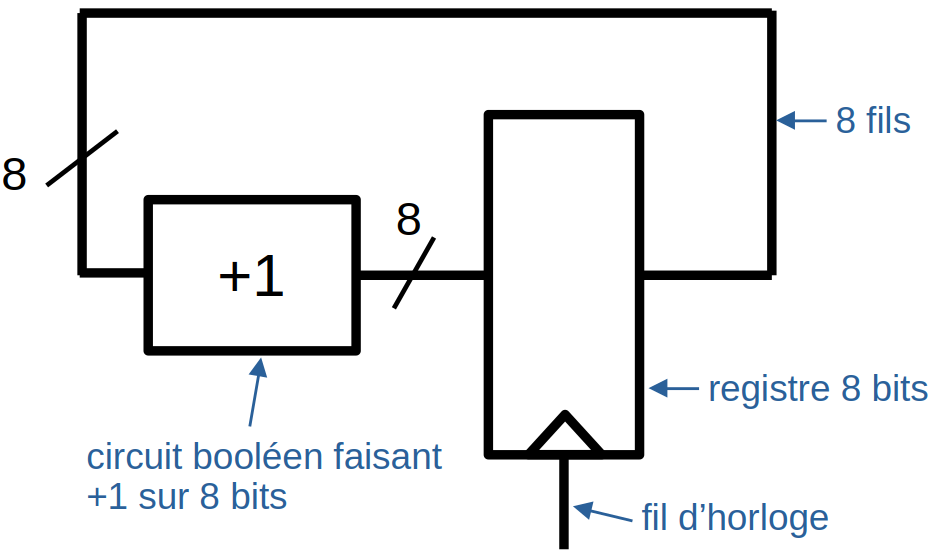
\includegraphics[width=0.4\linewidth]{lecon/23-archi-assembleur/compteur.png}}
\end{example}

\begin{rem}
	La fréquence de l'horloge détermine donc le temps minimal pour faire une opération dans un ordinateur. C'est ce que l'on dit quand on parle de processeur 4GHz (4 milliards de tac par secondes)
\end{rem}

\section{Modèle de Von Neuman}

\subsection{Le modèle}

\begin{definition}
	Une instruction est une opération à effectuer par le processeur sur des éléments de mémoire de l'ordinateur (registre, cache, RAM, disque dur, etc...).
\end{definition}

\begin{principe}
	Un ordinateur passe alors son temps à exécuter des instructions (qui modifie l'état de la mémoire)
\end{principe}

\begin{definition}
 	Le modèle de Von Neumann décrit le fonctionnement d'un ordinateur constitué : \begin{itemize}[label=$\bullet$] 
		\item d'un processeur qui lit les instructions en mémoire et les exécute. Il accède à la mémoire par blocs appelés mots mémoire. Pour cet accès, le processeur utilise un registre appelé compteur ordinal (Program Counter ou PC) qui contient une adresse en mémoire.
		\item La mémoire RAM adressé qui contient les programme à exécuter et les données. 
		\item Les périphériques d'entrée (clavier, souris, disque dur) et de sortie (écran, disque dur, haut parleur).
	 \end{itemize}
\end{definition}

\begin{rem}
	Une des spécificités de ce modèle est que les instructions sont des données comme les autres.
\end{rem}

\begin{personalise}[Schéma][Modèle de Von Neumann] CPU = processeur
	\begin{center}
		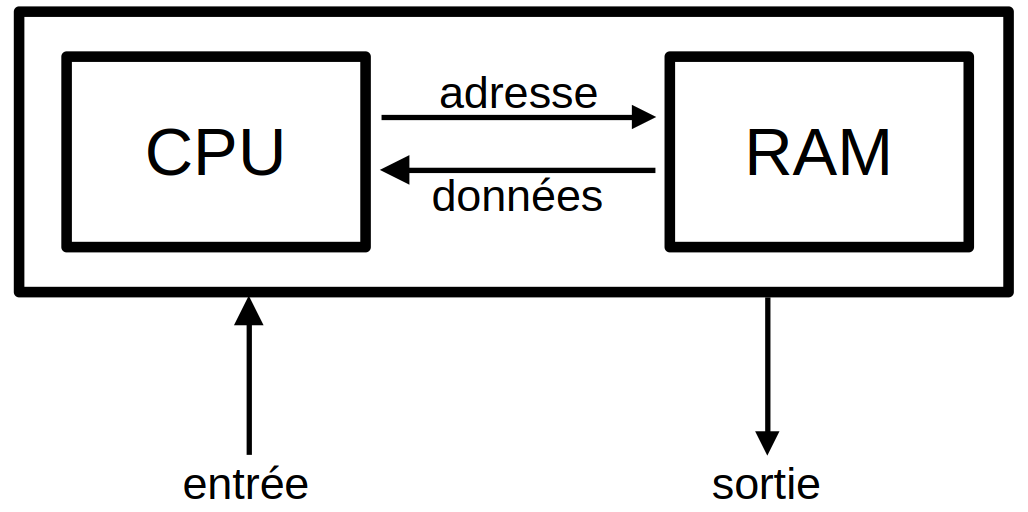
\includegraphics[width=0.5\linewidth]{lecon/23-archi-assembleur/modele_neumann.png}
	\end{center}
\end{personalise}

\begin{definition}[Cylce de Von Neumann]
	\begin{enumerate}
		\item \label{23-point1-cycle} Lire le mot mémoire qui commence à l'adresse PC
		\item Interpréter ce mot mémoire comme une instruction et l'exécuter
		\item Augmenter le PC pour passer à l'instruction suivante
		\item Retourner au \ref*{23-point1-cycle}
	\end{enumerate}
\end{definition}

\begin{rem}
	Quand vous avez plusieurs coeurs, il y a simplement plusieurs processeurs en parrallèle.
\end{rem}

\subsection{Registres et mémoire adressable}

Dans le modèle, la mémoire n'est pas dans le processeur. C'est la mémoire adressable (accessible par adresse).\\

Néanmoins, il y a aussi de la mémoire dans le processeur. Ce sont les registres. Quand un processeur veut exécuter une opération, il doit alors stocker les données dans des registres (les avoir en mémoire, sous la main), faire l'opération (et comme il doit stocker le résultat, le mettre dans un registre), puis renvoyer le résultat à la mémoire.

\begin{rem}
	Un processeur possède un registre stockant la valeur de PC.
\end{rem}

\section{Jeu d'instruction}

\subsection{Définition}

\begin{definition}
	Une instruction machine est une séquence de bits que le processeur peut interpréter et exécuter. Un jeu d'instructions (ISA) définit quelles sont les instructions supportées par le processeur, et la façon dont elles sont représentées en mémoire. L'ensemble de ces instructions machines forment le langage reconnu par le processeur, appelé langage machine. 
\end{definition}

\begin{rem}
	Tous les codes dans n'importe quel langage de programmation (exemple Python) doivent être traduits en langage machine pour être exécutés par le processeur. 
\end{rem}

\begin{proposition}
	En général, les jeux d'instructions gèrent les opérations suivantes : \begin{itemize}[label=$\bullet$]
		\item lire le contenu d'une case mémoire dans un registre, écrire le contenu d'un registre dans une case mémoire 
		\item opérations arithmétiques ou logiques (addition, et bit à bit, etc...)
		\item se déplacer dans le programme que l'on exécute (sauts)
	\end{itemize}
\end{proposition}

\begin{rem}
	Il exsite de nombreux ISA différents. On peut les diviser en deux catégories principales :
	
	CISC (complex instruction set computer) : plus d'instruction pouvant faire plus de choses mais donc plus longues (ex. x86 sur la plupart des ordinateurs)
	
	RISC (reduced instruction set computer) : moins d'instruction mais plus rapide et facile à implémenter (ex : RISC-V, ARM sur des téléphones).
\end{rem}

\subsection{Langage assembleur}

Une instruction est représentée en mémoire par un code en binaire. Par exemple, si les trois premiers bits sont des 0, on doit faire une opération arithmétique, puis si les deux suivants sont des 1, on fait une addition, etc. Néanmoins, cela est très peu lisible par l'être humain.

\begin{definition}
	Le langage assembleur représente le langage machine sous une forme lisible par un humain. C'est le langage de programmation de plus bas niveau.
\end{definition}

\begin{example}
	Exemple d'instruction classique : \begin{itemize}[label=$\bullet$]
		\item \texttt{load $r_i$ [$r_j$]}  : mets le contenu à l'addresse contenu dans $r_j$ dans le registre $r_i$
		\item \texttt{store $r_i$ [$r_j$]} : mets le contenu du registre $r_i$ dans la case d'adresse contenu dans $r_j$
		\item \texttt{add $r_i$ $r_j$ $r_k$} : ajoute le contenu des registres $r_i$ et $r_j$ pour le mettre dans le registre $r_k$
		\item \texttt{iload $r_i$ $x$} : mets la valeur $x$ dans le registre $r_i$
		\item \texttt{mv $r_i$ $r_j$} : mets la valeur du registre $r_i$ dans le registre $r_j$.
	\end{itemize}
\end{example}

\begin{example}
	Traduction en langage assembleur du code python «\texttt{z = x + y}»
	\begin{lstlisting}
iload <@$r_1$@> <@(adresse de x)@>
load <@$r_2$@> [<@$r_1$@>]
iload <@$r_1$@> <@(adresse de y)@>
load <@$r_3$@> [<@$r_1$@>]
add <@$r_1$@> <@$r_2$@> <@$r_3$@>
iload <@$r_1$@> <@(adresse de z)@>
store <@$r_2$@> [<@$r_1$@>]
	\end{lstlisting}
\end{example}

\begin{rem}
	Pour pouvoir exécuter des boucles et les si, on introduit de nouvelles instructions : \begin{itemize}[label=$\bullet$]
		\item \texttt{bge $r_1$ $r_2$ N} : va à la ligne $N$ si $r_1 \geq r_2$;
		\item \texttt{bgt}, \texttt{ble}, \texttt{beq}, \texttt{blt} (pour $>$, $\leq$, $=$, $<$)
		\item \texttt{jump $N$} : saute à la $N$-ième instruction du programme
	\end{itemize}
\end{rem}

\begin{example}
	Pour \texttt{while (i < n): i = i + 1}
	\begin{lstlisting}
0. iload <@$r_1$@> <@(adresse de x)@>
1. iload <@$r_2$@> <@(adresse de n)@>
2. load <@$r_2$@> [<@$r_2$@>]             // contient n
3. load <@$r_3$@> [<@$r_1$@>]             // contient i
4. bge <@$r_3$@> <@$r_2$@> 9
5. iload <@$r_4$@> 1
6. add <@$r_3$@> <@$r_3$@> <@$r_4$@>
7. store <@$r_3$@> [<@$r_1$@>]            // mettre à jour i
8. jump 3
9.
	\end{lstlisting}
\end{example}

\begin{rem}
	On peut faire beaucoup d'optimisation (par exemple en ne stockant $i$ que à la fin). Ce sont là d'importants sujet d'études (en compilation)
\end{rem}

\section{Gestion de la mémoire à plus haut niveau}

\begin{com}
	La raison de cette partie n'est pas uniquement de nous donner un développement mieux, mais également que c'est l'étape d'après dans la construction d'un ordinateur. Ici on commence à poser les premières briques du dessus. Surtout que c'est une étape cruciale de la compilation (passage de langage de plus haut niveau au code machine). Donc en tant qu'ouverture, tout en utilisant le langage assembleur ca parait cohérent.
\end{com}

Quand on exécute un programme qui n'est pas dans un langage assembleur, on a souvent besoin d’instruction de plus haut niveau, nous permettant d'allouer des variables, de faire des appels de fonctions imbriqués, etc. ce qui n'est à priori pas disponibles dans le langage assembleur tel quel.\\

Il faut alors traduire ces instructions de plus haut niveau en langage assembleur (i.e. compiler)

\begin{principe}
	Lors de l'exécution d'un processus, un espace mémoire en RAM lui est réservé. 
\end{principe}

\begin{minipage}{0.2\linewidth}
	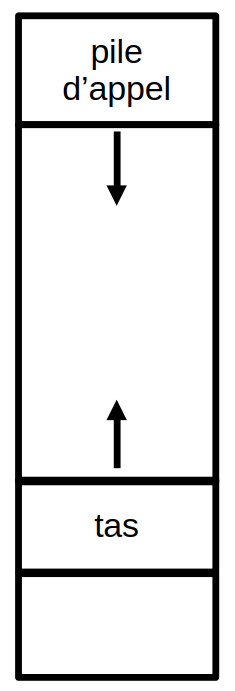
\includegraphics[height=6cm]{lecon/23-archi-assembleur/pile.png}
\end{minipage} \qquad
\begin{minipage}{0.6\linewidth}
	\begin{principe}    
		Le tas gère les données accessibles depuis tout le programme (malloc).
		
		Dans la pile, on met les variables locales à une fonction. A chaque nouvel appel, on empile de l'espace pour l'appel de fonction, que l'on enlève quand on return.
	\end{principe}
\end{minipage}

\paragraph{Développement :} Explication de la pile d'appel et implémentation en assembleur

%\makeatletter
%\renewcommand{\@chapapp}{Développement}
%\setcounter{chapter}{0}
%\makeatother
%\renewcommand\theHchapter{sec.\thechapter} %unique prefix
%
%\part{Développements}
 

\end{document}
